% VTID_en.tex — English version for arXiv hep-th
% Compiler: pdflatex
% Template: revtex4-2 (APS/PRD preprint style)

% NOTE: \RequirePackage{array}[=2016-10-06] causes conflict with booktabs.
% Apply only if arXiv compilation fails without it.
% \RequirePackage{array}[=2016-10-06]

\documentclass[
  aps,
  prd,
  preprint,
  groupedaddress,
  nofootinbib,
  longbibliography
]{revtex4-2}

% --- Mathematics ---
\usepackage{amsmath}
\usepackage{amssymb}
\usepackage{mathrsfs}  % \mathscr
\usepackage{amsthm}

% --- Theorem environments ---
% Numbered sequentially within each section: Definition 1.1, Proposition 1.2, ...
\newtheorem{definition}{Definition}[section]
\newtheorem{proposition}[definition]{Proposition}
\newtheorem{theorem}[definition]{Theorem}
\newtheorem{corollary}[definition]{Corollary}

% Remark: shares counter with definition/proposition/theorem
\theoremstyle{remark}
\newtheorem{remark}[definition]{Remark}

% --- Graphics ---
\usepackage{graphicx}

% --- Tables ---
\usepackage{booktabs}

% --- Hyperlinks ---
% revtex4-2 loads hyperref conditionally; explicit load for consistent behavior
\usepackage{hyperref}
\hypersetup{
  colorlinks=true,
  linkcolor=blue,
  citecolor=blue,
  urlcolor=blue,
  linktoc=page
}

% --- Custom commands ---
\newcommand{\Cex}{\mathcal{C}_{\mathrm{ex}}}
\newcommand{\N}{\mathcal{N}}
\newcommand{\AdS}{\mathrm{AdS}}
\newcommand{\CFT}{\mathrm{CFT}}
\newcommand{\SYM}{\mathrm{SYM}}
\newcommand{\dS}{\mathrm{dS}}

% =====================================================================
\begin{document}

\title{Vanishing theorems and incomplete deformations
  for vacuum data in \texorpdfstring{$\N=4$}{N=4} SYM}

\author{Yuichiro Nishi}
\email{nishi@yuichironishi.com}
\affiliation{Independent Researcher}

\date{March 2026}

\begin{abstract}
We prove that in the source-free, symmetric vacuum of $\N=4$
$SU(N)$ super Yang--Mills theory, the 1-point functions of all
operators in the family
$\Cex$---local scalar primaries, conserved currents, and the
energy-momentum tensor---vanish identically,
and that nonzero 1-point functions are permitted only under
deformations $S = S_{\mathrm{CFT}} + \Delta S_{\mathrm{def}}$.

This vanishing is sharply confined to local 1-point data.
Classifying observables into four layers, we show that
defects, information-theoretic quantities, and higher-point
correlators carry nontrivial data even in the undeformed vacuum
(scope-delimitation theorem).
The $\Lambda>0$ background fits into the deformation framework
as a geometric implementation.
Unifying the four-layer classification with the deformation
analysis, we show that representative deformations trigger
systematic responses across all four layers
(layer-resolved response theorem);
of the $20$ cells in the resulting matrix, $19$ are confirmed
by literature evidence, explicit computation, or the
QFT-on-de~Sitter framework.

The individual ingredients are separately known in quantum field
theory and the AdS/CFT correspondence.
What is new are structural facts emerging from their unification:
the vanishing is confined to Layer~I,
the deformation response is systematic rather than ad hoc,
and the sole unconfirmed cell
($\Lambda>0 \times$ Layer~II) is precisely locatable.
What remains open is not the correctness of the theorems but
the completeness of~$\Cex$ and its four-layer
extension---that is, the \emph{scope} of the claims made here.
\keywords{AdS/CFT correspondence, vanishing theorems, 1-point functions,
  conformal field theory, vacuum structure}
\end{abstract}

\maketitle
\clearpage
\tableofcontents

% =====================================================================
% INTRODUCTION
% =====================================================================
\section{Introduction}\label{sec:intro}

It is well known that 1-point functions of local operators
are strongly constrained in the symmetric vacuum of a conformal field
theory (CFT).
In a Poincar\'e-invariant, conformally invariant vacuum,
the 1-point function of a scalar primary with scaling dimension
$\Delta>0$ vanishes by the scale Ward identity~\cite{ref13,ref14};
that of a conserved current vanishes by Lorentz
invariance~\cite{ref13,ref14};
and that of the energy-momentum tensor on a flat background
vanishes by Lorentz invariance and the trace Ward
identity~\cite{ref5,ref13,ref14}.
On the bulk side of AdS/CFT, holographic renormalization shows
that the normalizable coefficient in a source-free pure-$\AdS$
background vanishes, giving a geometric expression of the same
conclusion~\cite{ref9,ref10,ref11,ref12}.

However, these vanishing results are usually stated separately
for each operator type, and no study has systematically addressed
the following questions:

\begin{enumerate}
\item[(i)]
Can these individual vanishing results be unified into a single
theorem for a defined operator family?

\item[(ii)]
When deformations---relevant deformations, finite temperature,
finite density, vacuum selection, $\Lambda>0$ backgrounds,
etc.---are introduced, how is the vanishing lifted, and can
this be classified systematically?

\item[(iii)]
What is the scope of the vanishing theorem---does it hold for
observables beyond local 1-point functions?

\item[(iv)]
How do observables outside the scope of the vanishing theorem
respond to deformations?
\end{enumerate}

This paper provides systematic answers to these questions
in the best-controlled standard example of AdS/CFT,
namely $\AdS_5\times S^5$ and its boundary dual $\N=4$
$SU(N)$ super Yang--Mills theory (SYM)~\cite{ref1,ref2,ref3,ref4}.

\bigskip

The main results of this paper are as follows.

\textbf{Vanishing theorem.}
The 1-point functions of all operators in the operator
family~$\Cex$, operationally defined in~\S\ref{sec:1},
vanish in the source-free, symmetric vacuum of the exact
conformal theory (Theorem~\ref{thm:vanishing}).
The proof is given from both the boundary Ward
identities~\cite{ref5,ref6,ref13,ref14} and the bulk
holographic renormalization~\cite{ref9,ref10,ref11,ref12}.

\textbf{Nonzero realization.}
Under a deformation $\Delta S_{\mathrm{def}}$,
\begin{equation}\label{eq:intro-deformation}
  S = S_{\mathrm{CFT}} + \Delta S_{\mathrm{def}}\,,
\end{equation}
---relevant deformations, finite temperature, finite chemical
potential, vacuum selection, time-dependent backgrounds, etc.---at
least one assumption supporting the vanishing theorem is violated,
and $\Cex$-relative nonzero 1-point functions are
permitted (Theorem~\ref{thm:nonzero}).
The concrete realization depends on the type of deformation
and the quantum numbers of the operator.

\textbf{$\Lambda>0$ background.}
The $\Lambda>0$ background does not preserve the assumptions
underlying the vanishing theorem, through the introduction
of an IR scale by the Hubble parameter~$H$, the Gibbons--Hawking
temperature $T_{\dS}=H/(2\pi)$ for a local observer, and the
modification of the source/response
dictionary~\cite{ref15,ref16,ref17,ref18,ref19,ref20,ref21}.
Thus $\Lambda>0$ is placed as a \emph{geometric deformation}
that breaks exact conformal invariance in a manner distinct
from matter-sector Lagrangian deformations
(Proposition~\ref{thm:lambda}).
The above results are collected in the unification
theorem (Theorem~\ref{thm:unification}).

\textbf{Four-layer classification and scope delimitation.}
We examine observables outside~$\Cex$---Wilson loops and other
defects, entanglement entropy, mutual information, and other
information-theoretic quantities, and higher-point
correlators---and classify observables into four layers
(Definition~\ref{def:four-layers}):
Layer~I (local 1-point data),
Layer~II (defect / nonlocal data),
Layer~III (information-theoretic data),
Layer~IV (correlation data).
The vanishing theorem is specific to Layer~I;
in the standard example $\AdS_5\times S^5 / \N=4$ SYM,
Layers~II--IV carry nontrivial data even in the symmetric
vacuum (Theorem~\ref{thm:scope}, scope-delimitation theorem).

\textbf{Layer-resolved response.}
Unifying the four-layer classification with the deformation
theory, we show that representative deformations---relevant
deformation, finite temperature, finite density, Coulomb branch,
and $\Lambda>0$---trigger systematic responses across all four
layers (Theorem~\ref{thm:layer-response}, layer-resolved response
theorem).
The activation of Layer~I is a deductive consequence of
Theorem~\ref{thm:nonzero}; the responses in Layers~II--IV
are confirmed by explicit computations for each
representative example, not by a general theorem.
Of the $20$ cells formed by representative deformations and
the four layers, $19$ are supported by literature evidence,
explicit computation, or the QFT-on-de~Sitter framework.
The sole unconfirmed cell is $\Lambda>0 \times$ Layer~II (defect),
which originates from the framework dependence of the observable
definition.

\textbf{Scope caveat.}
All theorems of this work are independent of the completeness
of~$\Cex$.
What remains open is not the correctness of the theorems but
the completeness of the adopted operator family~$\Cex$ and its
four-layer extension---that is, the \emph{scope} of the claims
made here.

\bigskip

The arguments in this paper are built on standard results
in quantum field theory and the AdS/CFT correspondence.
The vanishing theorem~(\S\ref{sec:2}) relies on the CFT Ward
identities~\cite{ref5,ref6,ref13,ref14} and holographic
renormalization~\cite{ref9,ref10,ref11,ref12}, each of which
is individually textbook material.
The description of nonzero realization~(\S\ref{sec:3})
uses finite-temperature and finite-density holographic
computations~\cite{ref4,ref39,ref42}, conformal perturbation
theory~\cite{ref14}, and the structure of the Coulomb
branch~\cite{ref4,ref6,ref7}.
The $\Lambda>0$ discussion~(\S\ref{sec:4}) is based on the
causal structure of de~Sitter space and the Gibbons--Hawking
temperature~\cite{ref15,ref17,ref20,ref21}.
The four-layer classification~(\S\ref{sec:6}) employs the exact
Wilson-loop result from Pestun
localization~\cite{ref31,ref29,ref30}, holographic entanglement
entropy~\cite{ref32,ref33}, and results on the modular
Hamiltonian~\cite{ref34}.
The layer-resolved response~(\S\ref{sec:7}) combines the
finite-temperature Wilson--Polyakov loop~\cite{ref40},
extensions of holographic entanglement entropy to finite
temperature and density~\cite{ref42}, holographic entanglement
entropy on the Coulomb branch~\cite{ref41}, and changes in
holographic entanglement entropy under RG flow~\cite{ref43}.

The individual ingredients are separately known;
the novelty lies in structural facts that emerge only from their
integration.
First, once the vanishing theorem is formulated for the operator
family~$\Cex$ as a whole
(Theorem~\ref{thm:vanishing}, Theorem~\ref{thm:unification}),
it admits a sharp scope boundary:
vanishing is confined to Layer~I, while Layers~II--IV carry
nontrivial data even in the exact conformal vacuum
(Theorem~\ref{thm:scope}).
This dichotomy is not visible from any single vanishing result
taken in isolation.
Second, the ``deformation~$\times$~layer'' matrix
(Theorem~\ref{thm:layer-response}) makes visible that the
deformation response across all four layers is systematic
rather than ad hoc, with $19$ of $20$ cells confirmed.
Third, the sole unconfirmed cell
($\Lambda>0 \times$ Layer~II) is identifiable precisely because
the matrix structure exists;
without it, this gap would not be locatable.

\bigskip

The paper is organized as follows.
In~\S\ref{sec:1}, we operationally define the exact conformal
theory and the operator family~$\Cex$ of candidate 1-point
observables, and delineate the propositions to be proved from
the completeness question to be left open.
In~\S\ref{sec:2}, we show that all 1-point functions of~$\Cex$
vanish in the conformal vacuum of~$\N=4$ SYM.
In~\S\ref{sec:3}, we systematize the conditions under which
1-point functions of~$\Cex$ can become nonzero under
deformations~$\Delta S_{\mathrm{def}}$.
In~\S\ref{sec:4}, we place the $\Lambda>0$ background as a
geometric deformation.
In~\S\ref{sec:5}, we collect the results of~\S\ref{sec:2}--\S\ref{sec:4}
into the unification theorem.
In~\S\ref{sec:6}, we examine observables outside~$\Cex$,
introduce the four-layer classification, and delimit the scope
of the vanishing theorem.
In~\S\ref{sec:7}, we unify the four-layer classification with
the deformation theory and establish the layer-resolved response
theorem.
In~\S\ref{sec:8}, we condense the conclusions of this work into
a final claim and state the falsification structure and the limits
of scope.

We begin in~\S\ref{sec:1} by introducing the definitions that
serve as the starting point.

% =====================================================================
% §1 DEFINITIONS AND FORMULATION
% =====================================================================
\section{Definitions and formulation}\label{sec:1}

\subsection{Purpose}\label{subsec:1-1}

The purpose of this paper is to formulate, in the most
controlled standard example of AdS/CFT---namely
$\AdS_5\times S^5$ and its boundary dual
$\N=4$ $SU(N)$ SYM~\cite{ref1,ref2,ref3,ref4}---the
proposition that \textbf{the quantities adopted in this work
as candidate 1-point observables vanish as 1-point functions
in the symmetric vacuum of an exact conformal theory, and
nontrivial 1-point vacuum data emerge only through symmetry
breaking, scale generation, or vacuum selection}.

What we call \emph{nontrivial vacuum data} in this paper does
not merely mean that operators can be defined on the Hilbert
space of the theory.
Nor does the nonvanishing of vacuum fluctuations or
higher-point correlators automatically qualify as nontrivial
vacuum data.
What is at issue is \textbf{whether the vacuum itself carries
a nontrivial bias, order, density, or production rate},
and this is determined fundamentally by the 1-point function.
In this sense, on the CFT side the Ward identities and vacuum
symmetry, and on the AdS side the structure of holographic
1-point functions, allow one to track rigorously what
``vanishes in the symmetric vacuum''~\cite{ref2,ref3,ref5,ref9,ref10}.

The central question of this paper can therefore be condensed to:

\begin{quote}
\textit{Can the symmetric vacuum of an exact conformal theory
carry a nonzero 1-point function?}
\end{quote}

Our answer is negative, relative to the adopted
operator family.
More precisely, in the conformal vacuum of~$\N=4$ SYM dual
to~$\AdS_5\times S^5$, the 1-point functions of the operator
family adopted as candidate 1-point observables vanish by
symmetry and the Ward
identities~\cite{ref1,ref2,ref3,ref4,ref5,ref6,ref7,ref13,ref14}.
Nontrivial 1-point vacuum data therefore arise not from the
exact conformal theory itself, but only through deformations,
symmetry breaking, or non-symmetric vacuum selection.

\subsection{The reference system
  \texorpdfstring{$\AdS_5\times S^5/\N=4$}{AdS5 x S5 / N=4} SYM}%
  \label{subsec:1-2}

To treat this problem with maximal rigor, we adopt type~IIB
string theory on $\AdS_5\times S^5$ and its boundary dual,
four-dimensional $\N=4$ SYM, as the reference
system~\cite{ref1,ref2,ref3,ref4}.
The reason is that this system implements the concept of an
exact conformal theory most explicitly.

The boundary theory $\N=4$ SYM is exactly superconformal
including quantum corrections, with
\begin{equation}\label{eq:beta-zero}
  \beta(g_{\mathrm{YM}}) = 0\,,
\end{equation}
so that the coupling constant does not run and the theory
does not dynamically generate an internal
scale~\cite{ref4,ref6,ref7}.
The theory possesses maximal supersymmetry and is consistently
defined under a large symmetry group including the
$R$-symmetry~\cite{ref4,ref6,ref7}.
The vacuum on a flat background is Poincar\'e-invariant and
conformally invariant, providing a unique reference vacuum
at zero source~\cite{ref4,ref6,ref13,ref14}.

On the bulk side, the corresponding vacuum is the maximally
supersymmetric background $\AdS_5\times S^5$; unless a source
is turned on, the near-boundary data corresponding to 1-point
functions of boundary operators are not
excited~\cite{ref2,ref3,ref9,ref10,ref11,ref12}.
Consequently, a \textbf{vanishing theorem based solely on
symmetry} and a \textbf{geometric vanishing via holography}
coincide.

This system is therefore the optimal testing ground for
describing, without ambiguity, the relationship between
exact conformal invariance and the vanishing of 1-point
functions.

\subsection{Definition of an exact conformal theory}\label{subsec:1-3}

In this paper, a theory satisfying all of the following
conditions is called an \textbf{exact conformal theory}:

\begin{enumerate}
\item The RG flow of the coupling constant vanishes:
  $\beta(g)=0$.
\item The vacuum is Poincar\'e-invariant.
\item The vacuum preserves scale or conformal symmetry.
\item No external scale has been introduced by an explicit
  relevant deformation.
\item In the source-free vacuum, no global symmetry is
  spontaneously broken.
\end{enumerate}

Under this definition, the conformal vacuum of $\N=4$ SYM
on $\mathbb{R}^{1,3}$ is the prototypical example of an
exact conformal
theory~\cite{ref4,ref6,ref7,ref13,ref14}.
The corresponding bulk description is the maximally symmetric
vacuum of source-free type~IIB string theory
on $\AdS_5\times S^5$~\cite{ref1,ref2,ref3,ref4}.

It should be emphasized that this definition of an exact
conformal theory is not a subjective description of solvability
or mathematical elegance, but an \textbf{operational concept
specified by the Ward identities, vacuum symmetry, and the
absence of scale generation}~\cite{ref6,ref13,ref14}.
As we shall show, the vanishing of the 1-point functions
treated in this paper follows mechanically from this definition.

\subsection{Operational definition of 1-point vacuum data}\label{subsec:1-4}

In this paper, the presence or absence of nontrivial vacuum
data is operationally determined by \textbf{the nonvanishing
of the 1-point function}~\cite{ref2,ref3,ref5,ref9,ref10}.

Concretely, 1-point vacuum data refers to any of the following:

\begin{itemize}
\item A nonzero scalar order parameter.
\item A nonzero conserved charge density.
\item A nonzero 1-point function of the energy-momentum tensor.
\item A nonzero expectation value of the divergence of a current.
\end{itemize}

Phenomenologically, these correspond respectively to, e.g.,
mass generation or selection of an ordered phase;
particle--antiparticle asymmetry or finite density;
deviation from a homogeneous vacuum;
and a production rate due to non-conservation processes.

However, when treating these within the framework of
$\AdS_5\times S^5/\N=4$ SYM, we do not directly embed
Standard Model operators.
Since $\N=4$ SYM contains neither fundamental quarks nor a
Higgs doublet, it would be theoretically inaccurate to take,
e.g., a baryon number operator or a Higgs VEV as direct
targets~\cite{ref4,ref7,ref8}.

Instead, we map 1-point vacuum data to an operator family
that is rigorously definable within $\N=4$ SYM:
\begin{equation}\label{eq:Cex-def}
  \mathcal{O}_\Delta^a(x),\qquad
  J_\mu^A(x),\qquad
  T_{\mu\nu}(x),\qquad
  \partial^\mu J_\mu^A(x)\,,
\end{equation}
and determine the presence or absence of nontrivial vacuum
data by the vanishing or nonvanishing of their 1-point
functions~\cite{ref5,ref9,ref10,ref11,ref12,ref13,ref14}.

This definition has two advantages.
First, all quantities are rigorously defined as operators in
the boundary CFT\@.
Second, via the AdS/CFT dictionary, they can be geometrically
re-expressed as near-boundary data of bulk
fields~\cite{ref2,ref3,ref9,ref10,ref11,ref12}.

\subsection{Precise form of the claims}\label{subsec:1-5}

Let us now restate the claims of this paper precisely.
What this paper demonstrates is not the vague assertion that
``nothing happens in an exact conformal theory,''
nor the overly strong claims that ``vacuum fluctuations do
not exist'' or ``correlators vanish.''

The claim of this paper takes the following specific form:

\begin{quote}
\textit{In the symmetric vacuum of an exact conformal theory,
the 1-point functions of candidate 1-point observables
belonging to the adopted operator family vanish.}
\end{quote}

Thus, for example,
\begin{equation}\label{eq:T00-vanish}
  \langle T_{00}(x)\rangle = 0
\end{equation}
is asserted, but
\begin{equation}\label{eq:T00T00-not-claimed}
  \langle T_{00}(x)\,T_{00}(y)\rangle = 0
\end{equation}
is \emph{not} asserted.
Indeed, the latter is generically
nonzero~\cite{ref5,ref13,ref14}.
Likewise, the existence of vacuum fluctuations and
higher-point correlators is distinguished from the
nonvanishing of 1-point vacuum data.

This distinction is essential for this paper.
The source-free, symmetric vacuum on $\AdS_5\times S^5$ is
quantum-mechanically nontrivial: it possesses a rich spectrum
and nontrivial correlation functions, yet the vacuum itself
carries no nonzero 1-point
function~\cite{ref1,ref2,ref3,ref4,ref5,ref6,ref7,ref9,ref10,ref11,ref12,ref13,ref14}.
What is at issue in this paper is \textbf{not whether the
quantum theory has content}, but \textbf{whether the vacuum
carries nontrivial 1-point data}.

Furthermore, it is important that the correctness of the
theorems in this paper does not depend on the adopted operator
family ``exhausting all necessary operators.''
What is rigorously shown is that \textbf{the 1-point function
vanishes for each element of the chosen operator family};
the completeness of that operator family is left as a separate
open question.
Thus, what is unresolved is not the correctness of the
theorems, but their \emph{scope}.

\subsection{Deformations and nonzero 1-point functions}\label{subsec:1-6}

Given an exact conformal theory, we consider a deformation
of the form
\begin{equation}\label{eq:deformation}
  S = S_{\mathrm{CFT}} + \Delta S_{\mathrm{def}}\,.
\end{equation}
Here $\Delta S_{\mathrm{def}}$ is a deformation that violates
at least one of the defining properties of the exact conformal
theory; examples include

\begin{itemize}
\item relevant deformation,
\item introduction of temperature or chemical potential,
\item change of boundary conditions,
\item vacuum selection,
\item supersymmetry breaking,
\item introduction of a curvature scale,
\item time-dependent backgrounds,
\end{itemize}
among
others~\cite{ref4,ref7,ref9,ref10,ref11,ref12,ref17,ref19,ref20,ref21,ref22,ref23,ref24,ref25,ref26,ref27}.

In such cases, the vanishing of the 1-point functions stated
in the previous section generically no longer holds.
For instance, scalar sources or the excitation of normalizable
modes permit $\langle\mathcal{O}_\Delta\rangle\neq 0$;
finite-temperature or finite-density states permit
$\langle T_{\mu\nu}\rangle\neq 0$ and
$\langle J_\mu\rangle\neq 0$~\cite{ref9,ref10,ref11,ref12}.
Similarly, if a symmetry is broken by an anomaly or explicitly,
$\langle\partial^\mu J_\mu\rangle$ can also become nonzero.

The structure of this paper is therefore twofold:

\begin{enumerate}
\item Show that in the symmetric vacuum of the exact conformal
  theory~$S_{\mathrm{CFT}}$, the 1-point functions of the
  candidate observables in the adopted operator family vanish.
\item Characterize how this vanishing is lifted by the
  deformation $\Delta S_{\mathrm{def}}$.
\end{enumerate}

The first task is the primary concern of this paper, and it
can be rigorously formulated using standard techniques of
AdS/CFT~\cite{ref2,ref3,ref9,ref10}.

With these definitions in hand, we proceed in
Section~\ref{sec:2} to show that every 1-point function
of~$\Cex$ vanishes in the conformal vacuum.

% =====================================================================
% §2 VANISHING THEOREM
% =====================================================================
\section{Rigorous formulation on
  \texorpdfstring{$\AdS_5\times S^5$}{AdS5 x S5}}\label{sec:2}

In this section, we rigorously formulate the 1-point vacuum data
introduced in Section~\ref{sec:1} on the conformal vacuum
of~$\N=4$ $SU(N)$ SYM and its $\AdS_5\times S^5$
dual~\cite{ref2,ref3,ref5,ref9,ref10,ref11,ref12}.
The main objective is to show that, in the source-free symmetric
vacuum of the exact conformal theory~$S_{\mathrm{CFT}}$,
the 1-point function of each element of the adopted operator
family vanishes, from both (i)~the boundary Ward identities
and (ii)~bulk holographic renormalization.

Throughout this section, the boundary spacetime is~$\mathbb{R}^{1,3}$,
the vacuum~$|0\rangle$ is Poincar\'e-invariant and conformally
invariant, and on the bulk side we adopt the source-free maximally
supersymmetric solution $\AdS_5\times
S^5$~\cite{ref1,ref2,ref3,ref4}.

We emphasize that the correctness of the propositions proved in
this section does not depend on the adopted operator family
``exhausting all necessary operators.''
What is shown is that \textbf{the 1-point function vanishes for
each element of the chosen operator family}; the completeness
of that family is left as a separate open question.

% -----------------------------------------------------------------
\subsection{Definition: the operator family of candidate 1-point
  observables}\label{subsec:2-1}

Following the discussion of Section~\ref{sec:1}, we define the
candidate 1-point observables to be treated rigorously in this paper
as an operator family that is well-defined within~$\N=4$ SYM.

\begin{definition}\label{def:Cex}
The operator family of candidate 1-point observables $\Cex$
(all local operators on the flat boundary~$\mathbb{R}^{1,3}$) is
defined by
\begin{equation}\label{eq:Cex}
  \Cex = \bigl\{\,
    \mathcal{O}_\Delta^a(x),\;
    J_\mu^A(x),\;
    T_{\mu\nu}(x),\;
    \partial^\mu J_\mu^A(x)
  \bigr\}\,,
\end{equation}
where
\begin{enumerate}
\item $\mathcal{O}_\Delta^a(x)$ is a local scalar primary operator
  with scaling dimension $\Delta>0$,
\item $J_\mu^A(x)$ is a conserved current corresponding to an
  exact global symmetry,
\item $T_{\mu\nu}(x)$ is the symmetric, conserved stress-energy
  tensor,
\item $\partial^\mu J_\mu^A(x)$ is the divergence of the current.
\end{enumerate}
The index $a$ labels a basis of scalar operators with the same
$\Delta$, and $A$ is a Lie algebra index of the global symmetry.
\end{definition}

\begin{remark}\label{rem:Delta-positive}
The condition $\Delta>0$ excludes the identity operator, whose
expectation value is trivially unity and carries no
vacuum-structure information.
\end{remark}

\begin{remark}\label{rem:Cex-not-SM}
This definition does not directly embed Standard Model operators
such as a baryon number operator or a Higgs doublet into~$\N=4$ SYM.
What is treated here is the operator family that uniformly describes
the abstract classes corresponding to their phenomenological
roles---nonzero scalar 1-point function, nonzero charge density,
nonzero stress tensor 1-point function, and nonzero current
non-conservation~\cite{ref4,ref7,ref8}.
\end{remark}

\begin{remark}\label{rem:Cex-relative}
In this paper, $\Cex$ is introduced as the operator family
providing candidate 1-point observables.
The theorems proved below are therefore $\Cex$-relative statements.
In particular, this paper shows
\begin{equation}\label{eq:Cex-vanishing}
  \forall\,\hat{\mathcal{O}}\in\Cex,\qquad
  \langle 0|\hat{\mathcal{O}}|0\rangle = 0\,,
\end{equation}
but does \emph{not} claim that ``all operators necessary for
nontrivial vacuum data are exhausted by~$\Cex$.''
What is unresolved is the completeness of the operator family,
which concerns not the correctness of the theorems but their scope.
\end{remark}

% -----------------------------------------------------------------
\subsection{Vanishing of 1-point functions: CFT side}\label{subsec:2-2}

We first establish the vanishing of 1-point functions on the
boundary CFT side.
The following propositions hold generally in any four-dimensional
CFT with a Poincar\'e-invariant, conformally invariant vacuum,
not only in~$\N=4$ SYM~\cite{ref5,ref6,ref13,ref14}.

\begin{proposition}\label{prop:scalar-vanish}
Let $\mathcal{O}_\Delta(x)$ be a local scalar primary with
$\Delta>0$.
In a Poincar\'e-invariant, scale-invariant vacuum~$|0\rangle$,
\begin{equation}\label{eq:scalar-vanish}
  \langle 0|\mathcal{O}_\Delta(x)|0\rangle = 0\,.
\end{equation}
\end{proposition}

\begin{proof}
By translation invariance,
$\langle 0|\mathcal{O}_\Delta(x)|0\rangle = C$ is a constant
independent of~$x$.
Under a scale transformation $x\mapsto\lambda x$, a scalar primary
transforms as
$\mathcal{O}_\Delta(x)\mapsto\lambda^{-\Delta}
\mathcal{O}_\Delta(\lambda x)$~\cite{ref13,ref14}.
If the vacuum is scale-invariant, then
\[
  C = \lambda^{-\Delta}\,C
  \qquad(\forall\,\lambda>0)\,.
\]
For $\Delta>0$, this forces $C=0$.
\end{proof}

\begin{corollary}\label{cor:scalar-N4}
In the conformal vacuum of~$\N=4$ SYM, for any nontrivial scalar
primary $\mathcal{O}_\Delta^a$,
\[
  \langle\mathcal{O}_\Delta^a(x)\rangle_0 = 0\,.
\]
In particular, for the $\tfrac{1}{2}$-BPS scalar chiral primaries
$\mathcal{O}_k^{(I_1\cdots I_k)}
= \mathrm{Tr}\bigl(\Phi^{(I_1}\cdots\Phi^{I_k)}\bigr)
-\text{traces}$
with $\Delta=k\ge 2$,
\[
  \langle\mathcal{O}_k^{(I_1\cdots I_k)}(x)\rangle_0
  = 0\,.
\]
See~\cite{ref4,ref5,ref6,ref7}.
\end{corollary}

\begin{proposition}\label{prop:current-vanish}
Let $J_\mu^A(x)$ be a global symmetry current.
In a Lorentz-invariant vacuum,
\begin{equation}\label{eq:current-vanish}
  \langle 0|J_\mu^A(x)|0\rangle = 0\,.
\end{equation}
\end{proposition}

\begin{proof}
By translation invariance,
$\langle J_\mu^A(x)\rangle_0 = v_\mu^A$ is a constant vector.
In a Lorentz-invariant vacuum, the existence of a nonzero constant
vector $v_\mu^A$ would single out a spacetime direction,
contradicting Lorentz invariance~\cite{ref13,ref14}.
Hence $v_\mu^A = 0$.
\end{proof}

\begin{corollary}\label{cor:charge-vanish}
In particular, the charge density vanishes:
$\langle J_0^A(x)\rangle_0 = 0$.
\end{corollary}

\begin{proposition}\label{prop:Tmunu-vanish}
In the conformal vacuum on a flat background~$\mathbb{R}^{1,3}$,
\begin{equation}\label{eq:Tmunu-vanish}
  \langle 0|T_{\mu\nu}(x)|0\rangle = 0\,.
\end{equation}
\end{proposition}

\begin{proof}
By translation and Lorentz invariance,
$\langle T_{\mu\nu}(x)\rangle_0 = c\,\eta_{\mu\nu}$
for some constant~$c$~\cite{ref13,ref14}.
In a four-dimensional CFT on a flat background,
the trace Ward identity gives
$\langle T^\mu{}_\mu(x)\rangle_0 = 0$~\cite{ref5,ref13,ref14}.
(In~$\N=4$ SYM, $a=c$; on flat~$\mathbb{R}^{1,3}$ both the Euler
density and the Weyl tensor vanish, so the trace anomaly is
identically zero.)
Therefore $0 = \eta^{\mu\nu}\langle T_{\mu\nu}\rangle_0 = 4c$,
so $c=0$ and $\langle T_{\mu\nu}(x)\rangle_0 = 0$.
\end{proof}

\begin{corollary}\label{cor:T00-vanish}
In particular, the local energy density vanishes:
$\langle T_{00}(x)\rangle_0 = 0$.
\end{corollary}

\begin{proposition}\label{prop:divJ-vanish}
If $J_\mu^A(x)$ is a conserved current corresponding to an exact
global symmetry, then the operator identity
$\partial^\mu J_\mu^A(x) = 0$ holds, and therefore
\begin{equation}\label{eq:divJ-vanish}
  \langle\partial^\mu J_\mu^A(x)\rangle_0 = 0\,.
\end{equation}
\end{proposition}

\begin{proof}
The Noether current of an exact symmetry is conserved.
The vacuum of~$\N=4$ SYM does not break this conservation law;
hence the result follows by taking the vacuum expectation
value~\cite{ref4,ref6,ref7}.
\end{proof}

\begin{remark}\label{rem:anomalous-current}
The above result concerns exactly conserved currents.
For anomalous or explicitly broken currents, the right-hand side
may include an anomaly functional or source-dependent term.
However, in the source-free conformal vacuum of~$\N=4$ SYM,
the current sector of~$\Cex$ is conserved and its 1-point function
vanishes~\cite{ref4,ref6,ref7}.
\end{remark}

% -----------------------------------------------------------------
\subsection{Generating-functional representation}\label{subsec:2-3}

The above propositions can also be expressed as variational
statements of the generating functional.
Introducing the boundary metric~$g^{(0)}_{\mu\nu}$, scalar
sources~$J_a$, and vector sources~$A_\mu^A$, define the connected
generating functional~\cite{ref2,ref3,ref5}
\begin{equation}\label{eq:W-def}
  W[J_a,A_\mu^A,g^{(0)}_{\mu\nu}]
  = \log Z[J_a,A_\mu^A,g^{(0)}_{\mu\nu}]\,.
\end{equation}
The 1-point functions are then
\begin{align}
  \langle\mathcal{O}_\Delta^a(x)\rangle
  &= \frac{1}{\sqrt{-g^{(0)}(x)}}\,
     \frac{\delta W}{\delta J_a(x)}\,,
  \label{eq:1pt-scalar-W}\\
  \langle J_A^\mu(x)\rangle
  &= \frac{1}{\sqrt{-g^{(0)}(x)}}\,
     \frac{\delta W}{\delta A_\mu^A(x)}\,,
  \label{eq:1pt-current-W}\\
  \langle T^{\mu\nu}(x)\rangle
  &= \frac{2}{\sqrt{-g^{(0)}(x)}}\,
     \frac{\delta W}{\delta g^{(0)}_{\mu\nu}(x)}\,.
  \label{eq:1pt-Tmunu-W}
\end{align}
At zero source on a flat background,
$J_a=0$, $A_\mu^A=0$, $g^{(0)}_{\mu\nu}=\eta_{\mu\nu}$,
the results of \S\ref{subsec:2-2} are summarized as
\begin{equation}\label{eq:W-vanish}
  \left.\frac{\delta W}{\delta J_a(x)}\right|_0 = 0\,,\qquad
  \left.\frac{\delta W}{\delta A_\mu^A(x)}\right|_0 = 0\,,\qquad
  \left.\frac{\delta W}{\delta g^{(0)}_{\mu\nu}(x)}\right|_0 = 0\,,
\end{equation}
where $|_0$ denotes evaluation at the above source-free, flat
background.

% -----------------------------------------------------------------
\subsection{Bulk side: holographic renormalization}\label{subsec:2-4}

We now rewrite the same propositions as statements about
near-boundary data on the AdS side.
By the AdS/CFT dictionary, the boundary generating functional
equals the bulk renormalized on-shell
action~\cite{ref2,ref3,ref9,ref10,ref11}:
\begin{equation}\label{eq:GKPW}
  W[J] = -S_{\mathrm{ren}}^{\mathrm{on\text{-}shell}}
    [\phi_{(0)}=J]
\end{equation}
(in Euclidean signature).
The 1-point functions of boundary operators are therefore
given by variations of the renormalized on-shell action with
respect to the boundary sources~\cite{ref9,ref10,ref11,ref12}.

\begin{proposition}\label{prop:bulk-scalar}
Let the bulk scalar~$\phi$ be dual to a boundary scalar
operator~$\mathcal{O}_\Delta$ of dimension~$\Delta$.
Then
\begin{equation}\label{eq:1pt-bulk-scalar}
  \langle\mathcal{O}_\Delta(x)\rangle
  = -\frac{1}{\sqrt{g_{(0)}(x)}}\,
    \frac{\delta S_{\mathrm{ren}}^{\mathrm{on\text{-}shell}}}
         {\delta\phi_{(0)}(x)}\,.
\end{equation}
In Fefferman--Graham coordinates,
\begin{equation}\label{eq:FG-metric}
  ds^2 = \frac{L^2}{z^2}\bigl(dz^2
    + g_{\mu\nu}(z,x)\,dx^\mu dx^\nu\bigr)\,,
  \qquad z\to 0\,,
\end{equation}
the near-boundary expansion of~$\phi$ reads
\begin{equation}\label{eq:phi-expansion}
  \phi(z,x) = z^{4-\Delta}\,\phi_{(0)}(x)
    + z^{\Delta}\,\phi_{(2\Delta-4)}(x) + \cdots\,,
\end{equation}
and the renormalized 1-point function is
\begin{equation}\label{eq:1pt-normalizable}
  \langle\mathcal{O}_\Delta(x)\rangle
  = (2\Delta-4)\,\phi_{(2\Delta-4)}(x)
    + \text{local counterterm contributions}
\end{equation}
\cite{ref9,ref10,ref11}.
\end{proposition}

\begin{remark}\label{rem:convention}
The numerical coefficient in~\eqref{eq:1pt-normalizable} is
convention-dependent.
What is essential for this paper is the structure that the
1-point function is determined by the normalizable
coefficient~$\phi_{(2\Delta-4)}$~\cite{ref9,ref10}.
\end{remark}

\begin{proposition}\label{prop:bulk-scalar-vanish}
In the source-free pure-$\AdS_5$ background, the scalar 1-point
function vanishes:
\begin{equation}\label{eq:bulk-scalar-vanish}
  \phi_{(0)}(x)=0
  \quad\text{and}\quad
  \phi_{(2\Delta-4)}(x)=0
  \quad\Longrightarrow\quad
  \langle\mathcal{O}_\Delta(x)\rangle = 0\,.
\end{equation}
\end{proposition}

\begin{proof}
Under the source-free condition, the maximally symmetric
pure-$\AdS_5$ solution carries no bulk scalar hair.
Consequently, the normalizable coefficient in the near-boundary
expansion also vanishes~\cite{ref9,ref10,ref11}.
The vanishing of the 1-point function then follows from the
definition~\eqref{eq:1pt-normalizable}.
\end{proof}

\begin{proposition}\label{prop:bulk-current}
Let the bulk gauge field $A_M^A$ be dual to the boundary
current~$J_\mu^A$.
Writing the near-boundary expansion as
\begin{equation}\label{eq:A-expansion}
  A_\mu^A(z,x)
  = A_\mu^{A(0)}(x) + z^2\,A_\mu^{A(2)}(x) + \cdots\,,
\end{equation}
the renormalized current 1-point function is
\begin{equation}\label{eq:1pt-bulk-current}
  \langle J_A^\mu(x)\rangle
  = -\frac{1}{\sqrt{g_{(0)}(x)}}\,
    \frac{\delta S_{\mathrm{ren}}^{\mathrm{on\text{-}shell}}}
         {\delta A_\mu^{A(0)}(x)}
  \propto A_A^{\mu(2)}(x)
    + \text{local terms}
\end{equation}
\cite{ref9,ref10,ref11}.
In the source-free pure-$\AdS_5$ background,
$A_\mu^{A(0)}(x)=0$ and $A_\mu^{A(2)}(x)=0$, so
$\langle J_A^\mu(x)\rangle = 0$.
\end{proposition}

\begin{proposition}\label{prop:bulk-Tmunu}
For the bulk metric in the Fefferman--Graham expansion
\begin{equation}\label{eq:g-expansion}
  g_{\mu\nu}(z,x) = g_{(0)\mu\nu}(x)
    + z^2\,g_{(2)\mu\nu}(x)
    + z^4\,g_{(4)\mu\nu}(x)
    + \cdots\,,
\end{equation}
the renormalized boundary stress tensor
is~\cite{ref9,ref10,ref11,ref12}
\begin{equation}\label{eq:1pt-Tmunu-bulk}
  \langle T_{\mu\nu}(x)\rangle
  = \frac{2}{\sqrt{-g_{(0)}(x)}}\,
    \frac{\delta W}{\delta g_{(0)}^{\mu\nu}(x)}
  = -\frac{2}{\sqrt{-g_{(0)}(x)}}\,
    \frac{\delta S_{\mathrm{ren}}^{\mathrm{on\text{-}shell}}}
         {\delta g_{(0)}^{\mu\nu}(x)}\,.
\end{equation}
For a four-dimensional boundary, this takes the form
\begin{equation}\label{eq:Tmunu-g4}
  \langle T_{\mu\nu}\rangle
  = \frac{L^3}{4\pi G_5}\,
    \bigl(g_{(4)\mu\nu}
    + X_{\mu\nu}[g_{(0)}]\bigr)\,,
\end{equation}
where $X_{\mu\nu}[g_{(0)}]$ is determined by local curvature
invariants of the boundary metric~\cite{ref9,ref10,ref11,ref12}.
On a flat boundary $g_{(0)\mu\nu}=\eta_{\mu\nu}$,
$X_{\mu\nu}=0$, and for pure $\AdS_5$,
$g_{(2)\mu\nu}=0$, $g_{(4)\mu\nu}=0$, so
$\langle T_{\mu\nu}(x)\rangle = 0$~\cite{ref9,ref10,ref11,ref12}.
\end{proposition}

% -----------------------------------------------------------------
\subsection{Agreement between the CFT and bulk sides}\label{subsec:2-5}

Collecting the results above, the vanishing of 1-point functions
from the boundary Ward identities and the vanishing of normalizable
coefficients in the source-free pure-$\AdS_5$ solution are two
expressions of the same
proposition~\cite{ref2,ref3,ref9,ref10,ref11,ref12}.

Schematically, the correspondence reads
\begin{equation}\label{eq:dictionary}
  \langle\mathcal{O}_\Delta\rangle
  \;\longleftrightarrow\;
  \phi_{(2\Delta-4)}\,,
  \qquad
  \langle J_\mu^A\rangle
  \;\longleftrightarrow\;
  A_\mu^{A(2)}\,,
  \qquad
  \langle T_{\mu\nu}\rangle
  \;\longleftrightarrow\;
  g_{(4)\mu\nu}\,.
\end{equation}
Thus, the vanishing of 1-point functions for the adopted operator
family~$\Cex$ is expressed as the Ward identities on the boundary
and as the absence of hair on the bulk side.

% -----------------------------------------------------------------
\subsection{Main theorem}\label{subsec:2-6}

Combining the above, the main result of this section is as follows.

\begin{theorem}[Vanishing theorem]\label{thm:vanishing}
Consider the Poincar\'e-invariant, conformally invariant
vacuum~$|0\rangle$ of~$\N=4$ $SU(N)$ SYM
on~$\mathbb{R}^{1,3}$, and its AdS/CFT dual, the maximally
supersymmetric vacuum of source-free type~IIB theory
on $\AdS_5\times S^5$~\cite{ref1,ref2,ref3,ref4}.
For the operator family defined in Definition~\ref{def:Cex},
\begin{equation}\label{eq:Cex-full}
  \Cex = \bigl\{\,
    \mathcal{O}_\Delta^a(x),\;
    J_\mu^A(x),\;
    T_{\mu\nu}(x),\;
    \partial^\mu J_\mu^A(x)
  \bigr\}\,,
\end{equation}
the following holds for any operator
$\hat{\mathcal{O}}\in\Cex$:
\begin{equation}\label{eq:main-vanishing}
  \langle 0|\hat{\mathcal{O}}|0\rangle = 0\,.
\end{equation}
More concretely,
\begin{equation}\label{eq:vanishing-all}
  \langle\mathcal{O}_\Delta^a(x)\rangle_0 = 0\,,\quad
  \langle J_\mu^A(x)\rangle_0 = 0\,,\quad
  \langle T_{\mu\nu}(x)\rangle_0 = 0\,,\quad
  \langle\partial^\mu J_\mu^A(x)\rangle_0 = 0\,.
\end{equation}
\end{theorem}

\begin{proof}
The scalar sector follows from
Propositions~\ref{prop:scalar-vanish}
and~\ref{prop:bulk-scalar-vanish}.
The current sector follows from
Propositions~\ref{prop:current-vanish},
\ref{prop:divJ-vanish}, and~\ref{prop:bulk-current}.
The stress-tensor sector follows from
Propositions~\ref{prop:Tmunu-vanish}
and~\ref{prop:bulk-Tmunu}.
Combining these yields the claim.
\end{proof}

% -----------------------------------------------------------------
\subsection{Remarks on scope}\label{subsec:2-7}

\begin{remark}\label{rem:scope-1}
The logical content of Theorem~\ref{thm:vanishing} is that the
1-point function of each element of the operator family~$\Cex$
vanishes in the source-free symmetric vacuum of the exact conformal
theory.
The correctness of this theorem does not depend on whether~$\Cex$
contains ``all operators necessary for nontrivial vacuum data.''
\end{remark}

Indeed, the proof of Theorem~\ref{thm:vanishing} is given
sector by sector using:
\begin{itemize}
\item the scale/conformal Ward identity for scalar
  primaries~\cite{ref13,ref14},
\item Lorentz invariance for vector
  currents~\cite{ref13,ref14},
\item Lorentz invariance and the trace Ward identity for the
  stress tensor~\cite{ref5,ref13,ref14},
\item the conservation law for the current
  divergence~\cite{ref4,ref6,ref7}.
\end{itemize}
Each argument acts individually on the adopted operator.
Therefore, as long as an operator~$\hat{\mathcal{O}}$ belongs
to~$\Cex$, the vanishing of its 1-point function is individually
established.

\begin{remark}\label{rem:divJ-rationale}
The inclusion of $\partial^\mu J_\mu^A$ in~$\Cex$ is motivated
by the deformation analysis of Section~\ref{sec:3}:
while identically zero in the exact conformal theory,
this operator can acquire a nonzero expectation value under
anomalous or explicit breaking
(Proposition~\ref{prop:anomaly}),
and its inclusion ensures that~$\Cex$ uniformly covers all
channels that can be activated by deformation.
\end{remark}

What this paper does \emph{not} show at this stage is the
completeness of the operator family in the sense that ``all
operators necessary for nontrivial vacuum data are exhausted
by~$\Cex$.''
The unresolved question is:
\begin{equation}\label{eq:completeness-open}
  \text{``All operators necessary for nontrivial vacuum data
  are exhausted by~$\Cex$.''}
\end{equation}
This is not an assumption needed for the proof of
Theorem~\ref{thm:vanishing}, but an additional question that
determines the ultimate scope of this work.

Consequently, what is rigorously established at this stage is
\begin{equation}\label{eq:established}
  \forall\,\hat{\mathcal{O}}\in\Cex,\qquad
  \langle 0|\hat{\mathcal{O}}|0\rangle = 0\,,
\end{equation}
while the proposition ``any 1-point vacuum datum can be expressed
as an element of~$\Cex$'' is deferred as a question for future
extension.

% -----------------------------------------------------------------
\subsection{What the theorem does not claim}\label{subsec:2-8}

The theorem of this section concerns the \textbf{vanishing of
1-point functions} and does not imply the triviality of the
theory as a whole.
In particular, the following are \emph{not} consequences of the
theorem:

\begin{enumerate}
\item Higher-point correlators vanish.
\item Vacuum fluctuations do not exist.
\item Nonlocal observables are trivial.
\item The same conclusion holds in excited or thermal states.
\end{enumerate}

In fact, generically
\begin{equation}\label{eq:2pt-nonzero}
  \langle T_{00}(x)\,T_{00}(y)\rangle_0 \neq 0\,,\qquad
  \langle\mathcal{O}_\Delta(x)\,
    \mathcal{O}_\Delta(y)\rangle_0 \neq 0\,,
\end{equation}
and the theory possesses a rich spectrum and nontrivial correlation
structure~\cite{ref5,ref13,ref14}.
What has been shown in this section is limited to the fact that,
for each element of the adopted operator family~$\Cex$,
\textbf{the symmetric vacuum itself carries no nonzero 1-point
order parameter or density}.

% -----------------------------------------------------------------
Having established the vanishing, we turn in
Section~\ref{sec:3} to the conditions under which
deformations lift it.

% =====================================================================
% §3 DEFORMATIONS AND NONZERO REALIZATION
% =====================================================================
\section{Deformation \texorpdfstring{$\Delta S_{\mathrm{def}}$}{Delta S def}
  and \texorpdfstring{$\Cex$}{Cex}-relative nonzero 1-point functions}\label{sec:3}

In Section~\ref{sec:2}, we showed that the 1-point function of
each element of the adopted operator family~$\Cex$ vanishes in
the source-free symmetric vacuum of the exact conformal
theory~$S_{\mathrm{CFT}}$.
As clarified in \S\ref{subsec:2-7}, the correctness of this result
does not depend on the completeness of~$\Cex$.
In this section, we systematize the types of deformations by which
this $\Cex$-relative vanishing theorem is lifted.

The goal is not to leave the result
$\langle\hat{\mathcal{O}}\rangle_0=0$ as a mere special case, but
to organize \textbf{which assumption must be violated for which
type of 1-point function in~$\Cex$ to become nonzero}.

Throughout this section, the deformation from the exact conformal
theory is written as
\begin{equation}\label{eq:deformation-sec3}
  S = S_{\mathrm{CFT}} + \Delta S_{\mathrm{def}}\,,
\end{equation}
where $\Delta S_{\mathrm{def}}$ violates at least one of the
defining properties of the exact conformal theory introduced
in \S\ref{subsec:1-3}.

% -----------------------------------------------------------------
\subsection{Necessary conditions for nonzero 1-point functions}%
  \label{subsec:3-1}

As follows from the proof in Section~\ref{sec:2},
the vanishing of the 1-point function for each element of~$\Cex$
relied principally on four conditions: (1)~translation invariance,
(2)~Lorentz invariance, (3)~scale/conformal invariance, and
(4)~exact current conservation together with the source-free
condition.

\begin{proposition}\label{prop:necessary}
Let $\hat{\mathcal{O}}\in\Cex$.
A necessary condition for
$\langle\hat{\mathcal{O}}\rangle\neq 0$ is that at least one
of the defining assumptions of the exact conformal theory is
violated.
\end{proposition}

\begin{proof}
Theorem~\ref{thm:vanishing} gives
$\langle\hat{\mathcal{O}}\rangle=0$ as long as all defining
assumptions hold.
The contrapositive yields the claim.
\end{proof}

\begin{remark}\label{rem:not-sufficient}
This is a necessary condition, not a sufficient one.
For instance, introducing a relevant deformation may still leave
certain 1-point functions vanishing, depending on residual
symmetry or the choice of source.
Below, we organize the specific circumstances under which each
sector of~$\Cex$ admits a nonzero 1-point function.
\end{remark}

% -----------------------------------------------------------------
\subsection{Relevant deformation and scalar 1-point function}%
  \label{subsec:3-2}

The most basic deformation is to couple a relevant operator to
the CFT\@.
For a scalar primary~$\mathcal{O}_\Delta$ with $\Delta<4$,
\begin{equation}\label{eq:relevant-def}
  \Delta S_{\mathrm{rel}}
  = \int d^4x\;\lambda\,\mathcal{O}_\Delta(x)\,,
\end{equation}
where $[\lambda]=4-\Delta>0$, so that $\lambda$ introduces an
explicit scale into the theory.
Scale/conformal symmetry is then lost, and the assumption of
Proposition~\ref{prop:scalar-vanish} no longer
holds~\cite{ref13,ref14}.

\begin{proposition}\label{prop:relevant}
Under the deformation
$S = S_{\mathrm{CFT}} + \int d^4x\,\lambda\,
\mathcal{O}_\Delta(x)$ with $\Delta<4$,
scale invariance is explicitly broken, and the scalar 1-point
function
$\langle\mathcal{O}_\Delta(x)\rangle$
need no longer vanish.
\end{proposition}

\begin{proof}
The relevant coupling~$\lambda$ carries mass dimension, providing
a scale available in the vacuum.
The scale Ward identity therefore no longer forces
$\langle\mathcal{O}_\Delta\rangle=0$~\cite{ref13,ref14}.
By dimensional analysis, a quantity of the form
$\lambda^{\Delta/(4-\Delta)}$ can be constructed, and when
$\lambda$ is the sole scale, the scalar 1-point function is
expected to exhibit such a scaling.
Hence, at least generically, the vanishing is no longer enforced.
\end{proof}

\begin{remark}\label{rem:relevant-W}
More precisely,
$\langle\mathcal{O}_\Delta(x)\rangle
= \delta W / \delta\lambda(x)$~\cite{ref2,ref3,ref5,ref9,ref10}.
If $\lambda$ is regarded as a constant source, the nonvanishing
of this 1-point function is tied to the $\lambda$-dependence
of the vacuum energy.
\end{remark}

% -----------------------------------------------------------------
\subsection{Finite temperature and nonzero stress tensor}%
  \label{subsec:3-3}

Introducing a finite temperature $T\neq 0$ is implemented by
compactifying the Euclidean time:
$\tau\sim\tau+\beta$, $\beta=T^{-1}$.
This selects a thermal state rather than the vacuum, breaking
both Lorentz invariance and scale invariance~\cite{ref4,ref7}.

\begin{proposition}\label{prop:finite-T}
In a thermal equilibrium state of~$\N=4$ SYM at $T\neq 0$,
the stress-tensor sector of~$\Cex$ satisfies
$\langle T_{\mu\nu}\rangle_T\neq 0$ in general.
In an isotropic thermal state,
\begin{equation}\label{eq:thermal-Tmunu}
  \langle T_{\mu\nu}\rangle_T
  = \mathrm{diag}(\varepsilon,p,p,p)\,,
\end{equation}
with the conformal equation of state
$\varepsilon = 3p$.
\end{proposition}

\begin{proof}
The temperature~$T$ introduces an explicit energy scale, and the
thermal state is not a vacuum, so Lorentz invariance is lost.
The assumption of Proposition~\ref{prop:Tmunu-vanish} therefore
fails~\cite{ref13,ref14}.
Since $\N=4$ SYM remains conformal, the thermal stress tensor
is traceless but need not
vanish~\cite{ref4,ref7}.
Isotropy and translation invariance constrain it to the above form.
\end{proof}

\begin{remark}\label{rem:AdS-Sch}
At strong coupling and large~$N$, this thermal state is dual
to an AdS-Schwarzschild black brane, whose holographic stress
tensor gives $\varepsilon\propto N^2 T^4$,
$p = \varepsilon/3$~\cite{ref3,ref4,ref12}.
\end{remark}

% -----------------------------------------------------------------
\subsection{Finite chemical potential and charge density}%
  \label{subsec:3-4}

For a global symmetry current~$J_\mu^A$, introducing a
time-component source defines a finite chemical potential:
\begin{equation}\label{eq:chem-pot}
  \Delta S_\mu = \int d^4x\;\mu_A\,J_0^A(x)\,.
\end{equation}
This permits a finite density in the vacuum and breaks Lorentz
invariance.

\begin{proposition}\label{prop:finite-mu}
With $\mu_A\neq 0$, the charge density in the current sector
of~$\Cex$ can become nonzero:
$\langle J_0^A(x)\rangle_\mu\neq 0$ in general.
\end{proposition}

\begin{proof}
$\mu_A$ is a constant source for~$J_0^A$, and
$\langle J_0^A(x)\rangle_\mu
= \delta W / \delta\mu_A(x)$~\cite{ref2,ref3,ref5,ref9,ref10}.
Finite $\mu_A$ singles out the time direction, breaking Lorentz
invariance, so Proposition~\ref{prop:current-vanish} does not
apply.
Thermodynamically, $\langle J_0^A\rangle$ equals the
$\mu_A$-derivative of the pressure or grand potential, and is
therefore generically nonzero.
\end{proof}

\begin{remark}\label{rem:AdS-RN}
On the AdS side, $\mu_A$ is implemented as the boundary value
$A_t^{A(0)}=\mu_A$ of the bulk gauge field.
The nonzero charge density corresponds to a nonzero normalizable
coefficient~$A_t^{A(2)}$~\cite{ref9,ref10,ref11}.
\end{remark}

% -----------------------------------------------------------------
\subsection{Vacuum selection and spontaneous symmetry breaking}%
  \label{subsec:3-5}

While Section~\ref{sec:2} fixed the conformal vacuum, the theory
may possess multiple vacuum branches.
$\N=4$ SYM itself has a Coulomb branch admitting adjoint scalar
VEVs~\cite{ref4,ref6,ref7}.

\begin{proposition}\label{prop:Coulomb}
In a Coulomb-branch vacuum of~$\N=4$ SYM, appropriate
gauge-invariant operators in the scalar sector of~$\Cex$ can
satisfy $\langle\mathcal{O}_\Delta(x)\rangle\neq 0$.
\end{proposition}

\begin{proof}
On the Coulomb branch, the eigenvalues of the adjoint
scalars~$\Phi^I$ are nonzero, introducing an intrinsic length
scale~\cite{ref4,ref6,ref7}.
Conformal symmetry is spontaneously broken, so the assumption
of Proposition~\ref{prop:scalar-vanish} fails.
Gauge-invariant operators of the form
$\mathrm{Tr}(\Phi^{(I_1}\cdots\Phi^{I_k)})$ can then have
generically nonzero VEVs.
\end{proof}

\begin{remark}\label{rem:Coulomb-holo}
In AdS/CFT, this corresponds to a Coulomb-branch geometry
departing from pure $\AdS_5\times
S^5$~\cite{ref1,ref4,ref7}.
The nonvanishing of boundary 1-point functions is equivalent
to normalizable deformations of bulk scalar modes, and chiral
primary VEVs have been computed
holographically~\cite{ref9,ref10,ref11,ref45}.
\end{remark}

% -----------------------------------------------------------------
\subsection{Explicit and anomalous current non-conservation}%
  \label{subsec:3-6}

In Section~\ref{sec:2}, exact global symmetry was assumed, giving
$\langle\partial^\mu J_\mu^A\rangle_0=0$.
When the current suffers an anomaly or explicit breaking, this
conclusion is lifted.

\begin{proposition}\label{prop:anomaly}
If a current~$J_\mu$ satisfies the anomaly equation
\begin{equation}\label{eq:anomaly}
  \partial^\mu J_\mu
  = \mathcal{A}[\text{background fields}]\,,
\end{equation}
and if the background fields are configured so that
$\mathcal{A}\neq 0$, then the divergence sector of~$\Cex$
satisfies
$\langle\partial^\mu J_\mu\rangle
= \langle\mathcal{A}\rangle\neq 0$.
\end{proposition}

\begin{proof}
Take the vacuum expectation value of the anomaly equation.
\end{proof}

\begin{remark}\label{rem:div-vs-density}
It is important that $\partial^\mu J_\mu\neq 0$
(non-conservation) and $\langle J_0\rangle\neq 0$ (finite
density) are distinct conditions.
To mimic baryogenesis-type phenomena, one typically needs not
only an anomaly but also CP violation, departure from
equilibrium, and a time-dependent background.
\end{remark}

% -----------------------------------------------------------------
\subsection{Time-dependent backgrounds}\label{subsec:3-7}

Time-dependent sources or curvature backgrounds destroy the
static nature of the vacuum.
In particular, in a cosmological background, the Poincar\'e
invariance of flat Minkowski space is lost.

\begin{proposition}\label{prop:time-dep}
In a time-dependent background
$g^{(0)}_{\mu\nu}(x)$, or with time-dependent
sources $J(x)$, $A_\mu(x)$, the $\Cex$-relative vanishing
theorem of Section~\ref{sec:2} does not hold in general.
In particular,
$\langle T_{\mu\nu}(x)\rangle$,
$\langle\mathcal{O}_\Delta(x)\rangle$, and
$\langle J_\mu(x)\rangle$
can become nonzero in a time-dependent manner.
\end{proposition}

\begin{proof}
Propositions~\ref{prop:scalar-vanish}--\ref{prop:divJ-vanish}
each assumed translation invariance, Lorentz invariance, or a
static vacuum.
In a time-dependent background these premises fail, and the
vanishing theorem does not apply.
\end{proof}

\begin{remark}\label{rem:dS-preview}
This point will become essential in the comparison with
$\Lambda>0$ backgrounds, especially de~Sitter-type geometries,
where the horizon, thermal properties, and time-dependent
coarse-graining do not permit the same structure of ``complete
vanishing of 1-point functions'' seen in the source-free conformal
vacuum of AdS~\cite{ref15,ref16,ref17,ref18,ref19,ref20,ref21,ref22,ref23,ref24,ref25,ref26,ref27}.
\end{remark}

% -----------------------------------------------------------------
\subsection{Bulk image of the deformations}\label{subsec:3-8}

Each deformation described above is expressed on the AdS side
as a deformation of the bulk geometry or bulk field
profile~\cite{ref3,ref4,ref9,ref10,ref11,ref12}.
The correspondence is summarized schematically as follows:

\begin{equation}\label{eq:bulk-image}
\begin{array}{c|c}
  \text{boundary deformation} & \text{bulk dual} \\[4pt]
  \hline\rule{0pt}{14pt}
  \lambda\,\mathcal{O}_\Delta
    & \phi_{(0)}\neq 0 \text{ or scalar hair} \\[4pt]
  T\neq 0
    & \text{AdS black brane / black hole} \\[4pt]
  \mu_A\neq 0
    & A_t^{A(0)}\neq 0,\; A_t^{A(2)}\neq 0 \\[4pt]
  \text{vacuum selection}
    & \text{normalizable moduli deformation} \\[4pt]
  g^{(0)}_{\mu\nu}(x)\neq\eta_{\mu\nu}
    & \text{nontrivial asymptotically AdS geometry}
\end{array}
\end{equation}

What these share is that the assumption of a ``source-free,
maximally symmetric pure-AdS geometry'' used in
Section~\ref{sec:2} breaks down.
As a result, the normalizable coefficients in the near-boundary
expansion become nonzero, and the boundary 1-point functions can
become nonzero~\cite{ref9,ref10,ref11,ref12}.

\begin{proposition}\label{prop:bulk-deformation}
If $\Delta S_{\mathrm{def}}$ induces a nontrivial classical
solution departing from pure $\AdS_5\times S^5$ on the bulk side,
then the corresponding boundary 1-point functions of~$\Cex$ can
generically become nonzero.
\end{proposition}

\begin{proof}
By holographic renormalization, boundary 1-point functions are
given by normalizable coefficients of bulk
fields~\cite{ref9,ref10,ref11}.
In solutions departing from pure AdS, these coefficients are
generically nonzero.
\end{proof}

% -----------------------------------------------------------------
\subsection{General theorem}\label{subsec:3-9}

Collecting the individual cases above, the deformation principle
of this paper is expressed as follows.

\begin{theorem}[Nonzero realization]\label{thm:nonzero}
Consider the theory obtained by adding a deformation
$\Delta S_{\mathrm{def}}$ to the exact conformal
theory~$S_{\mathrm{CFT}}$:
\begin{equation}\label{eq:deformed-theory}
  S = S_{\mathrm{CFT}} + \Delta S_{\mathrm{def}}\,.
\end{equation}
Suppose $\Delta S_{\mathrm{def}}$ violates at least one of
the assumptions supporting the $\Cex$-relative vanishing
theorem of Section~\ref{sec:2}---Poincar\'e invariance,
Lorentz invariance, scale/conformal invariance, the source-free
condition, or exact current conservation.
Then, for at least a part of~$\Cex$, nonzero 1-point functions
are permitted---the assumptions of the vanishing theorem no
longer hold.
For the finite-temperature, finite-density, Coulomb-branch,
and anomalous deformations, constructive realizations are
known; for time-dependent backgrounds, only the breakdown
of the vanishing conditions is established here.
More concretely, depending on the type of deformation, one or
more of the following can occur:
\begin{equation}\label{eq:nonzero-list}
  \langle\mathcal{O}_\Delta\rangle\neq 0\,,\quad
  \langle J_\mu\rangle\neq 0\,,\quad
  \langle T_{\mu\nu}\rangle\neq 0\,,\quad
  \langle\partial^\mu J_\mu\rangle\neq 0\,.
\end{equation}
\end{theorem}

\begin{proof}
Combine
Propositions~\ref{prop:relevant},
\ref{prop:finite-T},
\ref{prop:finite-mu},
\ref{prop:Coulomb},
\ref{prop:anomaly},
\ref{prop:time-dep},
and~\ref{prop:bulk-deformation}.
\end{proof}

\begin{remark}\label{rem:thm-nonzero-scope}
Like all results of this paper, Theorem~\ref{thm:nonzero} is
$\Cex$-relative (see \S\ref{subsec:1-5} and
\S\ref{subsec:2-7}).
\end{remark}

% -----------------------------------------------------------------
\subsection{Supplement: on sufficient conditions and genericity}%
  \label{subsec:3-10}

Theorem~\ref{thm:nonzero} is not the strong claim that
``if a deformation is introduced, then a specific 1-point function
necessarily becomes nonzero.''
Which 1-point function becomes nonzero depends on the symmetry
of the deformation, the boundary conditions, the choice of
state, and the quantum numbers of the coupled operator.

A related distinction concerns the level of evidence.
For finite temperature, finite density, Coulomb-branch,
and anomalous deformations, the nonvanishing is established
constructively---explicit formulas, thermodynamic identities,
or known holographic computations provide concrete nonzero
values.
For time-dependent backgrounds, the argument shows only that the
assumptions of the vanishing theorem fail; no explicit nonzero
value is computed in this paper.
The two levels---permission and constructive realization---are
both recorded in the statement of
Theorem~\ref{thm:nonzero}.

However, the important structure is the converse direction.
In a vacuum that is exactly conformal in the sense of
Section~\ref{sec:2}, all 1-point functions of~$\Cex$ vanish;
conversely, if a nonzero 1-point function for some element
of~$\Cex$ is observed, there must be a violation of the
assumptions of the exact conformal theory behind it.
In this sense, deformation is a necessary condition for
$\Cex$-relative nontrivial vacuum data, and---at least within the
scope of the adopted operator family---the emergence of nontrivial
vacuum data is tied to the violation of the assumptions of the
exact conformal theory.

% -----------------------------------------------------------------
We next apply this deformation framework to the~$\Lambda>0$
background in Section~\ref{sec:4}.

% =====================================================================
% §4 LAMBDA > 0 BACKGROUND
% =====================================================================
\section{Connection to the \texorpdfstring{$\Lambda>0$}{Lambda>0} background}%
  \label{sec:4}

In Section~\ref{sec:2} we showed that the 1-point function of every
element of the adopted operator family~$\Cex$ vanishes in the
conformal vacuum of~$\AdS_5\times S^5$ and its boundary
dual~$\N=4$~SYM\@.
In Section~\ref{sec:3} we organized how
this vanishing is lifted by deformations~$\Delta S_{\mathrm{def}}$.

The purpose of this section is to apply that general framework
to~$\Lambda>0$ backgrounds, in particular de~Sitter spacetime.
The aim is to clarify why the structure
``source-free, maximally symmetric, symmetric vacuum''
that held on~$\AdS_5\times S^5$ does not reproduce in the same
sense on de~Sitter geometry.
More precisely, the issue is not that de~Sitter admits ``no vacuum
at all,'' but that \textbf{the rigorous definition of observables
via a boundary generating functional, the source/response
dictionary, and the unambiguous treatment of the source-free vacuum
that were used in AdS/CFT are not implemented in the same form
for~$\Lambda>0$}~\cite{ref15,ref16,ref17,ref18,ref19,ref20,ref21}.
The purpose is not to prove new results about de~Sitter
quantum gravity, but to show that the vanishing-theorem
framework of this paper systematically identifies where and
how the assumptions of exact conformal invariance fail.

Below we first organize the difficulties in defining observables on
de~Sitter backgrounds, then describe the thermal properties arising
from the Gibbons--Hawking temperature and horizon.
We subsequently confirm that $H\sim\sqrt{\Lambda}$ acts as an IR
scale, and finally summarize, in the form of a theorem, how the
assumptions supporting the vanishing theorem are lost.

% -----------------------------------------------------------------
\subsection{Observables in de Sitter spacetime}\label{subsec:4-1}

The $d$-dimensional de~Sitter spacetime~$dS_d$ is the maximally
symmetric solution with positive cosmological
constant~$\Lambda>0$.
Using the de~Sitter radius~$L_{\dS}$ or the Hubble
rate~$H$, it is characterized
by~\cite{ref17,ref20,ref21}
\begin{equation}\label{eq:dS-curvature}
  R_{\mu\nu} = (d-1)\,H^2\,g_{\mu\nu}\,,
  \qquad
  \Lambda = \frac{(d-1)(d-2)}{2}\,H^2\,.
\end{equation}
Although geometrically maximally symmetric, an essential
difference from AdS appears when formulating quantum theory.
The first concerns \textbf{the definition of observables}.

In AdS, a timelike conformal boundary exists at spatial infinity,
on which boundary conditions, sources, and the generating
functional can be rigorously
defined~\cite{ref2,ref3,ref9,ref10,ref11}.
The GKPW-type dictionary used in Section~\ref{sec:2},
\begin{equation}\label{eq:GKPW-dS}
  W[J] = -S_{\mathrm{ren}}^{\,\mathrm{on\text{-}shell}}%
    [\phi_{(0)}=J]\,,
\end{equation}
relies on this structure.
In de~Sitter, the natural ``boundaries'' are the future
infinity~$\mathcal{I}^+$ and the past infinity~$\mathcal{I}^-$,
which differ in character from the timelike boundary of
AdS (see FIG.~\ref{fig:penrose})~\cite{ref16,ref17,ref18,ref19,ref20,ref21}.
Furthermore, a local observer is confined to a causal patch by
the cosmological horizon, so that the observable algebra of the
full theory cannot be given purely in terms of asymptotic data in
the same way as in
AdS~\cite{ref16,ref17,ref19,ref20,ref21}.

\begin{proposition}\label{prop:no-boundary-functional}
In de~Sitter spacetime, no timelike conformal boundary of the
AdS type exists.
Consequently, the source/response dictionary underlying the
vanishing theorem of Section~\ref{sec:2} cannot be applied
in standard form.
\end{proposition}

\begin{proof}
The GKPW dictionary of AdS is based on the specification of
boundary conditions and sources on the timelike conformal
boundary~\cite{ref2,ref3}.
In de~Sitter, $\mathcal{I}^\pm$ are not timelike, and a local
observer is confined to the interior of the horizon, so the
structure in which a single global boundary functional yields all
physical observables does not
hold~\cite{ref16,ref17,ref18,ref19,ref20,ref21}.
Hence the unambiguous formulation based on a boundary generating
functional of the type used in Section~\ref{sec:2} cannot be
applied as it stands.
\end{proof}

\begin{remark}\label{rem:dS-not-undefined}
This does not mean that all correlation functions or wavefunctions
are undefined in de~Sitter.
In fact, the late-time wavefunction, in-in correlators, static
patch observables, and dS/CFT-type proposals
exist~\cite{ref18,ref19,ref20,ref21,ref24,ref25}.
The claim here is the limited statement that the unambiguous
source/response dictionary for boundary 1-point functions of the
type supporting the rigorous theorem of Section~\ref{sec:2} is not
available in standard form.
\end{remark}

\begin{figure}[t]
\centering
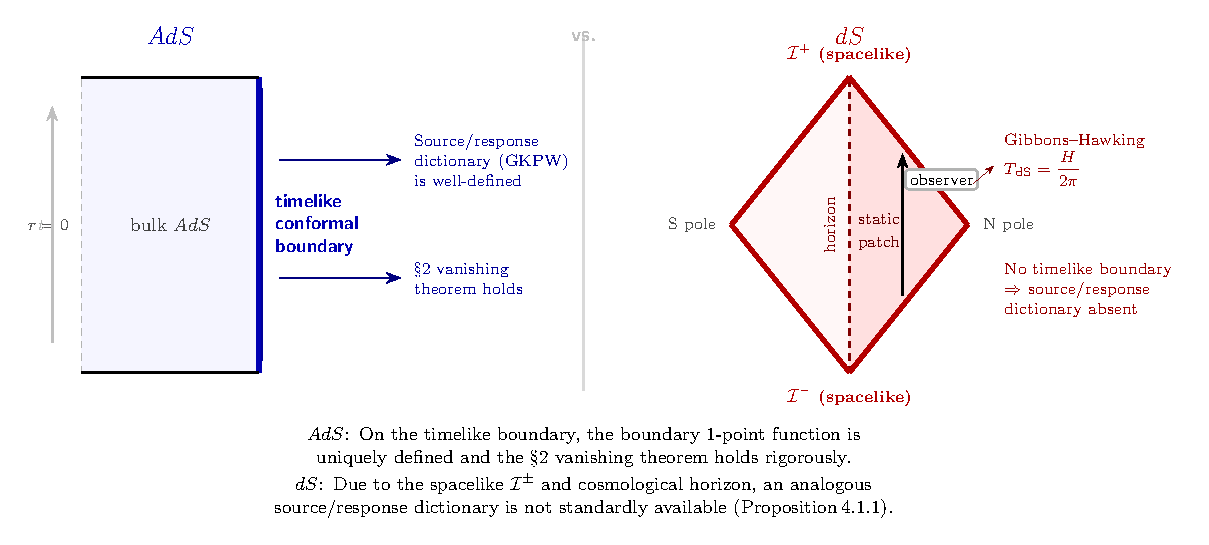
\includegraphics[width=\columnwidth]{figures/fig3_penrose_ads_ds_en.pdf}
\caption{Penrose diagrams for AdS (left) and de~Sitter (right).
  In AdS, the timelike conformal boundary supports a well-defined
  source/response dictionary (GKPW), and the vanishing theorem of
  Section~\ref{sec:2} holds rigorously.
  In de~Sitter, the boundaries~$\mathcal{I}^\pm$ are spacelike,
  and a local observer is confined to a static patch by the
  cosmological horizon at the Gibbons--Hawking
  temperature~$T_{\dS}=H/2\pi$.
  The standard source/response dictionary is not available
  (Proposition~\ref{prop:no-boundary-functional}).}
\label{fig:penrose}
\end{figure}

% -----------------------------------------------------------------
\subsection{Static patch and Gibbons--Hawking temperature}%
  \label{subsec:4-2}

The second essential feature of de~Sitter is that every geodesic
observer possesses a cosmological
horizon~\cite{ref15,ref17,ref20,ref21}.
In static patch coordinates the metric takes the form
\begin{equation}\label{eq:static-patch}
  ds^2 = -(1-H^2 r^2)\,dt^2
         +\frac{dr^2}{1-H^2 r^2}
         +r^2\,d\Omega_{d-2}^2\,,
\end{equation}
and the horizon is located at $r=H^{-1}$~\cite{ref17,ref20,ref21}.
Quantum-mechanically, this horizon is associated with a
temperature~\cite{ref15}
\begin{equation}\label{eq:GH-temp}
  T_{\dS} = \frac{H}{2\pi}\,.
\end{equation}

\begin{proposition}\label{prop:GH-thermal}
In the static patch of de~Sitter spacetime, restricting the
Bunch--Davies vacuum to a local observer yields a reduced state
that behaves as a thermal density matrix at
temperature~$T_{\dS}=H/(2\pi)$.
\end{proposition}

\begin{proof}
The Bunch--Davies vacuum is a de~Sitter-invariant Gaussian state
whose two-point function, through Euclidean continuation, possesses
periodicity $\beta=2\pi/H$~\cite{ref22,ref23}.
Since the KMS condition with respect to static patch time is
satisfied, the reduced density matrix for the local observer
is a thermal state at
temperature~$T_{\dS}=H/(2\pi)$~\cite{ref15,ref17,ref20,ref21,ref23}.
\end{proof}

\begin{corollary}\label{cor:no-cold-vacuum}
A local observer in de~Sitter does not observe an ``empty'' pure
vacuum in general, but a thermally coarse-grained state.
\end{corollary}

\begin{remark}\label{rem:thermal-interpretation}
This fact does not directly negate the structure used in
Section~\ref{sec:2}---``vanishing of the 1-point function in
the source-free, Poincar\'e-invariant, symmetric vacuum''---but
it drastically changes its \textbf{physical interpretation}.
Whereas in AdS the source-free vacuum can be treated even locally
as a cold reference state, in de~Sitter the same notion of
``cold emptiness'' cannot be assigned to the static patch
observer~\cite{ref15,ref16,ref17,ref20,ref21,ref23}.
\end{remark}

% -----------------------------------------------------------------
\subsection{Introduction of an IR scale by \texorpdfstring{$H$}{H}}%
  \label{subsec:4-3}

At the core of the scalar 1-point function vanishing theorem
in Section~\ref{sec:2} was the absence of any intrinsic scale
in the conformal vacuum~\cite{ref13,ref14}.
In de~Sitter, even if the UV side of the theory is scale-invariant,
the background curvature itself introduces a length
scale~\cite{ref17,ref20,ref21}
\begin{equation}\label{eq:H-scale}
  H^{-1}\,.
\end{equation}

\begin{proposition}\label{prop:IR-scale}
In quantum field theory on a de~Sitter background, the Hubble
rate~$H$ acts as an external IR scale, so that the argument for
the vanishing of the 1-point function based on the scale Ward
identity in flat-space CFT does not hold in general.
\end{proposition}

\begin{proof}
In a flat-space CFT, $\langle\mathcal{O}_\Delta\rangle=0$
follows from the absence of any scale that could build a quantity
of dimension~$\Delta>0$~\cite{ref13,ref14}.
On a de~Sitter background, the curvature
radius~$H^{-1}$ is given as background data, so by dimensional
analysis a quantity
\begin{equation}\label{eq:dim-analysis}
  \langle\mathcal{O}_\Delta\rangle \sim c\,H^\Delta
\end{equation}
can be constructed~\cite{ref17,ref20,ref21}.
The vanishing proof based on scale invariance in
Section~\ref{sec:2} therefore does not apply.
\end{proof}

\begin{remark}\label{rem:nonzero-conditional}
Whether $\langle\mathcal{O}_\Delta\rangle$ actually becomes
nonzero depends on the quantum numbers of the operator, the
renormalization scheme, the choice of state, and the way
de~Sitter symmetry is
realized~\cite{ref20,ref21,ref22,ref23,ref26,ref27}.
What matters here is that \textbf{the enforcing power that
requires it to vanish is lost}.
\end{remark}

% -----------------------------------------------------------------
\subsection{Mismatch between de Sitter symmetry and the local observer}%
  \label{subsec:4-4}

Since de~Sitter spacetime is maximally symmetric as a whole, one
might object that ``in a symmetric vacuum the 1-point function
should still vanish.''
However, the key point is that the \textbf{global dS-invariant
state} and the \textbf{physical state actually accessible to the
static patch observer} are not
identical~\cite{ref17,ref20,ref21}.

Even though the global Bunch--Davies state is de~Sitter-invariant,
its restriction to the static patch is a thermal mixed
state~\cite{ref15,ref17,ref20,ref21,ref23}.
The quantity relevant to a local observer is therefore not the
global vacuum expectation value but the expectation value with
respect to the patch-restricted density matrix.

\begin{proposition}\label{prop:global-not-enough}
In de~Sitter, global de~Sitter invariance alone does not guarantee
the vanishing of 1-point functions for a local observer.
\end{proposition}

\begin{proof}
Global de~Sitter invariance refers only to the symmetry of the
total state; the accessible algebra of a local observer is
restricted to the causal patch~\cite{ref17,ref20,ref21}.
This restriction maps the global pure state to a local mixed state.
For a mixed thermal state, the vanishing theorem of
Section~\ref{sec:2}, which was established for the
Lorentz-invariant vacuum, cannot be applied as it
stands~\cite{ref15,ref17,ref20,ref21,ref23}.
\end{proof}

\begin{remark}\label{rem:stress-tensor-observer}
For example, in the static patch thermal state the local
expectation value of the stress-energy tensor is defined in an
observer-dependent manner, and the renormalized stress tensor can
become nonzero.
At a minimum, the argument of Section~\ref{sec:2}---concluding
uniquely~$0$ from symmetry alone---breaks
down~\cite{ref17,ref20,ref21}.
\end{remark}

% -----------------------------------------------------------------
\subsection{In-in formalism and late-time observables}%
  \label{subsec:4-5}

In a cosmological background, the natural observables are often
defined not via an AdS-type boundary S-matrix or a Euclidean
generating functional but via the Schwinger--Keldysh in-in
formalism~\cite{ref24,ref25}.
That is, for an initial state~$|\Psi_{\mathrm{in}}\rangle$,
the expectation value at time~$t$ is
\begin{equation}\label{eq:in-in}
  \langle\mathcal{O}(t)\rangle
  = \langle\Psi_{\mathrm{in}}|\,
    \bar{T}\exp\!\Bigl(i\!\int_{t_0}^{t}\!H_I(t')\,dt'\Bigr)\,
    \mathcal{O}_I(t)\,
    T\exp\!\Bigl(-i\!\int_{t_0}^{t}\!H_I(t')\,dt'\Bigr)
    |\Psi_{\mathrm{in}}\rangle\,,
\end{equation}
where $T$ and~$\bar{T}$ denote time-ordering and
anti-time-ordering respectively~\cite{ref24,ref25}.
In this framework, the dynamics of a time-dependent background
and horizon are directly reflected in the observables.

\begin{proposition}\label{prop:in-in}
In a de~Sitter-type cosmological background, the natural
observables are given by in-in expectation values or late-time
wavefunction coefficients rather than by boundary 1-point
functions.
\end{proposition}

\begin{proof}
In de~Sitter, asymptotic scattering states or timelike boundary
sources of the AdS type are not available in general, while
cosmological observables are defined as expectation values at
finite times or at late
times~\cite{ref19,ref20,ref21}.
These are described by the Schwinger--Keldysh formalism or the
wavefunction of the universe~\cite{ref24,ref25}.
\end{proof}

\begin{remark}\label{rem:late-time}
This point clearly separates the ``vanishing of the 1-point
function in a source-free CFT vacuum'' of Section~\ref{sec:2}
from the cosmologically relevant late-time observables such as
$\langle\delta\rho/\rho\rangle$ and
$\langle\zeta\zeta\rangle$~\cite{ref24,ref25}.
In de~Sitter, the nontriviality of the vacuum manifests not only
at the level of 1-point functions but also through effective
classicalization via mode freezing and decoherence.
\end{remark}

% -----------------------------------------------------------------
\subsection{\texorpdfstring{$\Lambda>0$}{Lambda>0} viewed as a
  deformation}\label{subsec:4-6}

In light of the general framework of Section~\ref{sec:3}, the
$\Lambda>0$ background can be regarded as a type of geometric
deformation~$\Delta S_{\mathrm{def}}$ of the exact conformal
theory~$S_{\mathrm{CFT}}$.
What this deformation breaks is
principally~\cite{ref15,ref16,ref17,ref18,ref19,ref20,ref21}:
\begin{enumerate}
\item flat-space Poincar\'e invariance,
\item the definition of observables based on a global timelike
  boundary,
\item the interpretation of the local state as a cold vacuum,
\item scalelessness.
\end{enumerate}

\begin{definition}\label{def:Lambda-deformation}
Let the geometric deformation due to a positive cosmological
constant be denoted by
\begin{equation}\label{eq:DeltaS-Lambda}
  \Delta S_{\Lambda>0}\,.
\end{equation}
This is regarded as a deformation that breaks the assumptions of
the exact conformal theory not only in the matter sector but also
in the definition of observables, the local interpretation of the
vacuum, and the IR structure.
\end{definition}

\begin{proposition}\label{prop:Lambda-breaks}
$\Delta S_{\Lambda>0}$ breaks at least the following assumptions
supporting the vanishing theorem
(Theorem~\ref{thm:vanishing}): the flat-space implementation of scale
invariance, the source/response dictionary based on a timelike
boundary, and the cold-vacuum interpretation for a local observer.
\end{proposition}

\begin{proof}
The flat-space implementation of scale invariance is broken by
the introduction of the Hubble
scale~$H$~\cite{ref17,ref20,ref21}.
The source/response dictionary based on a timelike boundary is
replaced by the causal structure of
de~Sitter~\cite{ref16,ref17,ref18,ref19,ref20,ref21}.
The vacuum as seen by a local observer appears as a thermal state
with the Gibbons--Hawking temperature, so the cold-vacuum
interpretation is
lost~\cite{ref15,ref17,ref20,ref21,ref23}.
\end{proof}

% -----------------------------------------------------------------
\subsection{Main result: AdS-type exact conformal invariance is
  not stable in de Sitter}\label{subsec:4-7}

Combining all of the above, the main claim of this section is
summarized as follows.

\begin{proposition}\label{thm:lambda}
The vanishing theorem for 1-point functions in
the source-free, symmetric vacuum
(Theorem~\ref{thm:vanishing}) does not hold
in the same form on a~$\Lambda>0$ background in general.
More specifically, on a de~Sitter-type background:
\begin{enumerate}
\item the AdS/CFT-type timelike boundary source/response dictionary
  is not available in standard form,
\item for a static patch observer, the vacuum appears as a thermal
  state at temperature~$T_{\dS}=H/2\pi$,
\item the background curvature~$H$ introduces an IR scale, and
\item cosmological observables are defined by in-in expectation
  values or the late-time wavefunction,
\end{enumerate}
so that the assumptions supporting the vanishing theorem of
Section~\ref{sec:2} are not preserved.
Consequently, the~$\Lambda>0$ background is understood as a form
of the deformation~$\Delta S_{\mathrm{def}}$ in the sense of
Section~\ref{sec:3}.
\end{proposition}

\begin{proof}
Follows by combining
Propositions~\ref{prop:no-boundary-functional},
\ref{prop:GH-thermal},
\ref{prop:IR-scale},
\ref{prop:global-not-enough},
\ref{prop:in-in},
and~\ref{prop:Lambda-breaks}.
\end{proof}

\begin{remark}\label{rem:lambda-status}
Unlike Theorem~\ref{thm:vanishing}, which is deduced from Ward
identities and holographic renormalization, the above proposition
is a structural observation about the failure of assumptions
on a~$\Lambda>0$ background.
It does not compute a specific nonzero 1-point function on
de~Sitter; it identifies why the vanishing theorem cannot be
applied.
\end{remark}

% -----------------------------------------------------------------
\subsection{Physical implications}\label{subsec:4-8}

Proposition~\ref{thm:lambda} does not assert that ``in de~Sitter,
all 1-point functions of~$\Cex$ necessarily become nonzero.''
What it asserts is that the framework of the exact conformal
theory that held on~$\AdS_5\times S^5$ becomes structurally
unstable for~$\Lambda>0$.
This instability is consistent with the emergence of nontrivial
observables in cosmological
backgrounds~\cite{ref15,ref16,ref17,ref18,ref19,ref20,ref21,
  ref22,ref23,ref24,ref25,ref26,ref27}.

In particular, in inflationary or quasi-de~Sitter backgrounds,
quantum fluctuations freeze after horizon crossing and become
the seeds of late-time density
perturbations~\cite{ref24,ref25}.
What is essential there is not the 1-point function that vanished
in Section~\ref{sec:2} but \textbf{the IR scale~$H$}, the
\textbf{time-dependent background}, the \textbf{coarse-graining
by the horizon}, and the \textbf{in-in observable}
framework~\cite{ref15,ref16,ref17,ref18,ref19,ref20,ref21,
  ref22,ref23,ref24,ref25,ref26,ref27}.
In a de~Sitter-type universe it is more natural to regard the
background geometry itself as already implementing the deformation,
rather than to take the ``cold symmetric vacuum of an exact
conformal theory'' as the starting point.

% -----------------------------------------------------------------
In Section~\ref{sec:5} we collect the results of
Sections~\ref{sec:2}--\ref{sec:4} into the unification theorem.

% =====================================================================
% §5 UNIFICATION THEOREM
% =====================================================================
\section{Unification theorem}\label{sec:5}

In Section~\ref{sec:2} we showed that the 1-point function of
every element of the adopted operator family~$\Cex$ vanishes in
the source-free, symmetric vacuum of the exact conformal
theory~$S_{\mathrm{CFT}}$.
In Section~\ref{sec:3} we organized how
this vanishing is lifted by deformations~$\Delta S_{\mathrm{def}}$.
In Section~\ref{sec:4} we showed that, on a~$\Lambda>0$
background---in particular de~Sitter spacetime---the source-free,
symmetric vacuum structure of~$\AdS_5\times S^5$ is not stably
realized in the same
sense~\cite{ref1,ref2,ref3,ref4,ref5,ref6,ref7,ref8,ref9,ref10,
  ref11,ref12,ref13,ref14,ref15,ref16,ref17,ref18,ref19,ref20,
  ref21,ref22,ref23,ref24,ref25,ref26,ref27}.

The purpose of this section is to assemble these results into a
single unified proposition.
It is essential to separate clearly the part that holds as a
theorem from the physical interpretation placed on top of it.
What holds as a theorem is the structure that, \textbf{relative
to the adopted operator family~$\Cex$, all 1-point functions
vanish in the symmetric vacuum of the exact conformal theory,
and their nonvanishing is permitted once a deformation is
introduced}.

% -----------------------------------------------------------------
\subsection{Unification theorem}\label{subsec:5-1}

We collect the notation introduced in the preceding sections.
Write the exact conformal theory as
$S_{\mathrm{CFT}}$,
with the canonical example being~$\N=4$ $SU(N)$ SYM
on~$\mathbb{R}^{1,3}$ and its holographic dual, source-free
type~IIB string theory on~$\AdS_5\times
S^5$~\cite{ref1,ref2,ref3,ref4}.
The operator family of candidate 1-point observables is
\begin{equation}\label{eq:Cex-recall}
  \Cex = \bigl\{\,
    \mathcal{O}_\Delta^a(x),\;
    J_\mu^A(x),\;
    T_{\mu\nu}(x),\;
    \partial^\mu J_\mu^A(x)
  \bigr\}\,,
\end{equation}
where $\mathcal{O}_\Delta^a$ is a scalar primary with
$\Delta>0$, $J_\mu^A$ is an exact global symmetry current, and
$T_{\mu\nu}$ is the stress
tensor~\cite{ref4,ref5,ref6,ref7,ref13,ref14}.

\begin{theorem}\label{thm:unification}
In the source-free, symmetric vacuum~$|0\rangle$ of the exact
conformal theory~$S_{\mathrm{CFT}}$, for every
$\hat{\mathcal{O}}\in\Cex$,
\begin{equation}\label{eq:unif-vanish}
  \langle 0|\hat{\mathcal{O}}|0\rangle = 0\,.
\end{equation}
On the other hand, in the theory
\begin{equation}\label{eq:deformed-theory-unif}
  S = S_{\mathrm{CFT}} + \Delta S_{\mathrm{def}}\,,
\end{equation}
if $\Delta S_{\mathrm{def}}$ breaks at least one of the
assumptions supporting the vanishing theorem of
Section~\ref{sec:2}, then for at least part of~$\Cex$,
\begin{equation}\label{eq:unif-nonzero}
  \langle\hat{\mathcal{O}}\rangle_S \neq 0
\end{equation}
is permitted; for the specific deformations listed in
Theorem~\ref{thm:nonzero}, constructive realizations are known.
Furthermore, the~$\Lambda>0$ background can be regarded as a
geometric implementation of such~$\Delta S_{\mathrm{def}}$
through the definition of observables, the thermal properties
of the local vacuum, and the introduction of the IR
scale~$H$~\cite{ref15,ref16,ref17,ref18,ref19,ref20,ref21,
  ref22,ref23,ref24,ref25,ref26,ref27}.
\end{theorem}

\begin{proof}
The first claim follows from
Theorem~\ref{thm:vanishing}.
The second from Theorem~\ref{thm:nonzero}.
The third from Proposition~\ref{thm:lambda}.
\end{proof}

% -----------------------------------------------------------------
\subsection{%
  \texorpdfstring{$\Cex$}{C\_ex}-relative
  definition of 1-point vacuum data}\label{subsec:5-2}

The theorems of this paper are meaningful when 1-point vacuum data
are adopted as the class of 1-point functions belonging
to~$\Cex$.
Under this definition, 1-point vacuum data are nontrivial
physical quantities carried by the vacuum or state itself, and
their presence or absence is determined by the nonvanishing of
the expectation value~\cite{ref2,ref3,ref5,ref9,ref10}.

\begin{definition}\label{def:nontrivial-data}
A state~$\rho$ is said to possess \textbf{$\Cex$-relative
nontrivial vacuum data} with respect to
$\hat{\mathcal{O}}\in\Cex$ if
\begin{equation}\label{eq:nontrivial-data}
  \langle\hat{\mathcal{O}}\rangle_\rho \neq 0\,.
\end{equation}
\end{definition}

\begin{remark}\label{rem:not-particles}
This definition differs from the presence or absence of particle
content, of higher-point correlation functions, or of vacuum
fluctuations~\cite{ref5,ref13,ref14}.
The claim of this paper thus rests on the operational definition
\begin{equation}\label{eq:operational-equiv}
  \text{$\Cex$-relative nontrivial vacuum data}
  \quad\Longleftrightarrow\quad
  \text{nonzero 1-point function of some }
  \hat{\mathcal{O}}\in\Cex\,.
\end{equation}
\end{remark}

\begin{remark}\label{rem:completeness-not-assumed}
Here $\Cex$ is a natural operator family providing candidate
1-point observables, but its completeness---i.e., whether all
operators necessary for nontrivial vacuum data are exhausted by
this family---is not assumed in this paper.
What is rigorously shown is the fact that, for every operator
belonging to~$\Cex$, the 1-point function vanishes in the
symmetric vacuum of the exact conformal theory.
\end{remark}

% -----------------------------------------------------------------
\subsection{Corollary: an exact conformal theory carries no
  \texorpdfstring{$\Cex$}{C\_ex}-relative nontrivial vacuum
  data}\label{subsec:5-3}

\begin{corollary}\label{cor:no-data}
The source-free, symmetric vacuum of the exact conformal
theory~$S_{\mathrm{CFT}}$ carries no nontrivial vacuum data
in the sense of the operator family~$\Cex$ adopted in this paper.
\end{corollary}

\begin{proof}
By Theorem~\ref{thm:unification}, all 1-point functions
of~$\Cex$ vanish.
\end{proof}

\begin{remark}\label{rem:not-trivial-theory}
This corollary does not mean that the exact conformal theory is
physically trivial.
The theory still possesses a nontrivial spectrum, higher-point
correlation functions, Wilson loops, scattering amplitudes, and
a holographic dual
geometry~\cite{ref1,ref2,ref3,ref4,ref5,ref6,ref7,ref9,ref10,
  ref11,ref12,ref13,ref14}.
What is claimed is merely that, \textbf{with respect to the
quantities belonging to the adopted operator family~$\Cex$, the
vacuum itself carries no nonzero 1-point order parameter or
density}.
\end{remark}

% -----------------------------------------------------------------
\subsection{Corollary: an observed nonzero quantity implies
  breakdown of exact conformal invariance}\label{subsec:5-4}

Reading Theorem~\ref{thm:unification} in the converse direction,
an observed nonzero 1-point quantity for some operator
in~$\Cex$ implies that at least one of the assumptions of the
exact conformal theory is violated.

\begin{corollary}\label{cor:converse}
If, in a state~$\rho$, some
$\hat{\mathcal{O}}\in\Cex$ satisfies
\begin{equation}\label{eq:converse}
  \langle\hat{\mathcal{O}}\rangle_\rho \neq 0\,,
\end{equation}
then $\rho$ is not the source-free, symmetric vacuum of the
exact conformal theory assumed in Section~\ref{sec:2}.
More precisely, at least one of the following is violated:
Poincar\'e invariance, Lorentz invariance, scale/conformal
invariance, the source-free condition, or exact current
conservation.
\end{corollary}

\begin{proof}
This is the contrapositive of Theorem~\ref{thm:vanishing}.
\end{proof}

\begin{remark}\label{rem:converse-core}
This corollary constitutes the physical core of the vanishing
theorem and the deformation principle of this paper.
The ``deformation'' referred to here does not mean a mathematical
inconsistency or theoretical pathology.
What it means is that, \textbf{at least within the scope
of~$\Cex$, the vacuum does not fully preserve symmetry,
scalelessness, and the source-free condition}.
\end{remark}

% -----------------------------------------------------------------
\subsection{Position of the \texorpdfstring{$\Lambda>0$}{Lambda>0}
  background}\label{subsec:5-5}

Incorporating the results of Section~\ref{sec:4}, a positive
cosmological constant implements the departure from exact
conformal invariance in a manner different from a matter-sector
Lagrangian deformation: it is a geometric deformation acting
through the background geometry, the definition of observables,
and the thermal nature of the local
state~\cite{ref15,ref16,ref17,ref18,ref19,ref20,ref21,
  ref22,ref23,ref24,ref25,ref26,ref27}.

\begin{proposition}\label{prop:Lambda-position}
A~$\Lambda>0$ background does not remain within exact conformal
invariance in the flat-space conformal vacuum sense.
Hence a cosmological background with~$\Lambda>0$ can be regarded
as a geometric~$\Delta S_{\mathrm{def}}$ in the sense of this
paper.
\end{proposition}

\begin{proof}
By Proposition~\ref{thm:lambda}, the assumptions supporting the
vanishing theorem are not preserved on a de~Sitter background.
\end{proof}

\begin{remark}\label{rem:Lambda-not-nonzero}
This proposition does not assert that ``in de~Sitter a specific
1-point function of~$\Cex$ necessarily becomes nonzero.''
What it asserts is the structural statement that the framework
of the exact conformal theory that held on~$\AdS_5\times S^5$
cannot be carried over as it stands to a~$\Lambda>0$
background~\cite{ref15,ref16,ref17,ref18,ref19,ref20,ref21}.
\end{remark}

% -----------------------------------------------------------------
\subsection{Final formulation}\label{subsec:5-6}

In light of the above, the core proposition of this paper can
be summarized in the following concise form.

\begin{definition}\label{def:vacuum-data-set}
For the adopted operator family~$\Cex$, define the
\textbf{$\Cex$-relative vacuum data} of a state~$\rho$ by
\begin{equation}\label{eq:E-Cex}
  \mathfrak{E}_{\Cex}(\rho)
  = \bigl\{\,
      \langle\hat{\mathcal{O}}\rangle_\rho
      \;\big|\;
      \hat{\mathcal{O}}\in\Cex
    \bigr\}\,.
\end{equation}
\end{definition}

\noindent
Hereafter, $\rho_0 := |0\rangle\langle 0|$ denotes the density
matrix of the source-free, symmetric vacuum.

\begin{theorem}\label{thm:final}
For the source-free, symmetric vacuum~$\rho_0$ of the exact
conformal theory,
\begin{equation}\label{eq:E-zero}
  \mathfrak{E}_{\Cex}(\rho_0) = \{0\}\,.
\end{equation}
On the other hand, for a state~$\rho_{\mathrm{def}}$ obtained
by a deformation~$\Delta S_{\mathrm{def}}\neq 0$, in general
\begin{equation}\label{eq:E-nonzero}
  \mathfrak{E}_{\Cex}(\rho_{\mathrm{def}}) \neq \{0\}
\end{equation}
is permitted.
\end{theorem}

\begin{proof}
The former is the first part of
Theorem~\ref{thm:unification}, and the latter is its second part.
\end{proof}

% -----------------------------------------------------------------
\subsection{Physical interpretation}\label{subsec:5-7}

Here, for the first time, we can give a minimal physical
interpretation to the rigorous results obtained so far.
The exact conformal theory~$S_{\mathrm{CFT}}$ is mathematically
closed and is the theory most tightly controlled by symmetry.
Yet, precisely because of that exact conformal invariance, its
symmetric vacuum carries---at least within the scope
of~$\Cex$---no nonzero 1-point order parameter, no nonzero
density, and no nonzero production rate.
Therefore, $\Cex$-relative nontrivial vacuum data emerge not from
the exact conformal theory itself but only through
its breaking, deformation, or vacuum selection.

This interpretation can be written in formulae; the content of
this paper is summarized in the following schema:
\begin{align}
  S_{\mathrm{CFT}}
  &\quad\Longrightarrow\quad
  \forall\,\hat{\mathcal{O}}\in\Cex,\;
  \langle\hat{\mathcal{O}}\rangle = 0\,,
  \label{eq:schema-vanish}\\[6pt]
  S_{\mathrm{CFT}}+\Delta S_{\mathrm{def}}
  &\quad\Longrightarrow\quad
  \exists\,\hat{\mathcal{O}}\in\Cex
  \;\text{such that}\;
  \langle\hat{\mathcal{O}}\rangle \neq 0
  \;\text{is allowed.}
  \label{eq:schema-nonzero}
\end{align}

In this sense, nontrivial vacuum data in the sense of this paper
are understood not as the mere well-definedness of the theory
but as the fact that, \textbf{with respect to the adopted
operator family~$\Cex$, the state carries nontrivial 1-point
data not enforced by symmetry}.

% -----------------------------------------------------------------
\subsection{Limitations and open problems}\label{subsec:5-8}

The discussion in this paper has a clear domain of applicability.

First, the 1-point vacuum data treated here are limited to
1-point functions belonging to~$\Cex$.
Since much of cosmological structure formation and
classicalization is described through 2-point functions,
non-Gaussianity, decoherence, and open-system dynamics, an
extension is needed to incorporate them into the present
framework~\cite{ref24,ref25}.

Second, the discussion of the~$\Lambda>0$ background does not
presuppose a rigorous duality of the AdS/CFT type; it is a
structural argument based on the standard difficulties in
defining observables in de~Sitter and on horizon
thermality~\cite{ref15,ref16,ref17,ref18,ref19,ref20,ref21}.
The results of Section~\ref{sec:4} should therefore be understood
not as rigorous holographic theorems in the sense of
Section~\ref{sec:2} but as a \textbf{systematic organization
of the reasons for the breakdown of exact conformal invariance}.

Third, a more concrete dictionary is needed between the
abstract operator family~$\Cex$ and Standard Model phenomena
such as baryon asymmetry, electroweak symmetry breaking, and
cosmological perturbations.
This is a task to be refined in the context of top-down
compactifications, the introduction of flavor branes, or
holographic effective field
theory~\cite{ref4,ref7,ref8}.

Fourth, the most essential open problem is the completeness
of~$\Cex$: whether all operators necessary for nontrivial vacuum
data are exhausted by~$\Cex$ is unproven in this paper.
Consequently, the conclusion rigorously established at the
present stage is $\Cex$-relative.

% -----------------------------------------------------------------
\subsection{Summary of this section}\label{subsec:5-9}

In this paper, $\AdS_5\times S^5/\N=4$~SYM was adopted as
the canonical example of an exact conformal theory, and we showed
that the 1-point function of every element of the operator
family~$\Cex$ defined there vanishes in the source-free, symmetric
vacuum~\cite{ref1,ref2,ref3,ref4,ref5,ref6,ref7,ref8,ref9,ref10,
  ref11,ref12,ref13,ref14}.
Next, we systematized that these 1-point functions belonging
to~$\Cex$ can become nonzero once deformations
$\Delta S_{\mathrm{def}}$ such as relevant deformations, finite
temperature, finite density, vacuum selection, and time-dependent
backgrounds are
introduced~\cite{ref3,ref4,ref9,ref10,ref11,ref12}.
Furthermore, we showed that a~$\Lambda>0$ background can be
regarded as a geometric implementation of such a deformation
through the definition of observables, the thermal horizon,
and the introduction of an IR
scale~\cite{ref15,ref16,ref17,ref18,ref19,ref20,ref21,
  ref22,ref23,ref24,ref25,ref26,ref27}.

The final conclusion of this paper is therefore:
\begin{equation}\label{eq:box1}
  \fbox{\parbox{0.88\columnwidth}{%
    The symmetric vacuum of the exact conformal theory
    carries no $\Cex$-relative nontrivial 1-point data.}}
\end{equation}
\begin{equation}\label{eq:box2}
  \fbox{\parbox{0.88\columnwidth}{%
    The emergence of $\Cex$-relative nontrivial 1-point
    data requires a deformation~$\Delta S_{\mathrm{def}}$.}}
\end{equation}

This claim is rigorously formulated on~$\AdS_5\times S^5$
insofar as 1-point vacuum data are adopted as the class of
1-point functions belonging to~$\Cex$.
A cosmological background with~$\Lambda>0$ is then positioned
as an example in which that exact conformal invariance is
geometrically
broken~\cite{ref15,ref16,ref17,ref18,ref19,ref20,ref21,
  ref22,ref23,ref24,ref25,ref26,ref27}.

At the same time, this paper does not claim that the totality of
operators necessary for nontrivial vacuum data is exhausted
by~$\Cex$.
This paper should therefore be understood not as the final form
of a completed classification but as a \textbf{rigorous first
step toward the vanishing theorem and the deformation principle,
with the $\Cex$-relative vanishing theorem at its core}.

In the following sections we address the open problem of the
completeness of~$\Cex$ left in this section, introducing the
``four-layer structure of vacuum data'' that includes observables
not belonging to~$\Cex$---nonlocal operators, information-theoretic
quantities, and higher-point correlation
functions (Section~\ref{sec:6}).
We then unify this four-layer classification with the deformation
theory developed up to this section, systematically describing how
each layer responds under
deformation (Section~\ref{sec:7}).

% =====================================================================
% §6 FOUR-LAYER CLASSIFICATION
% =====================================================================
\section{Generalized observables and the scope of the 1-point
  framework}\label{sec:6}

In Section~\ref{sec:5} we stated the unification theorem relative
to the adopted operator family~$\Cex$ and showed that all 1-point
functions of~$\Cex$ vanish in the source-free, symmetric vacuum
of the exact conformal theory.
At the same time, in \S\ref{subsec:5-8} the completeness
of~$\Cex$---whether all operators necessary for nontrivial
vacuum data are exhausted by this family---was left as an open
problem.

The purpose of this section is to address that open problem
directly.
Concretely, we examine observables not belonging
to~$\Cex$---nonlocal operators, information-theoretic quantities,
and higher-point correlation functions---and rigorously determine
whether the vanishing theorem of Section~\ref{sec:2} holds for
them.

The main result is as follows: the vanishing theorem of
Section~\ref{sec:2} is \textbf{a result specific to local,
1-point, intrinsic order parameters} and cannot in general be
extended to nonlocal, relational, or information-theoretic
quantities.
This fact does not indicate a weakness of the theorem but, on
the contrary, sharply characterizes the nature of the 1-point
vacuum data that the vanishing theorem captures.

% -----------------------------------------------------------------
\subsection{Setup: conditions for the vanishing theorem to hold}%
  \label{subsec:6-1}

We recall the proof structure on which the vanishing theorem
(Theorem~\ref{thm:vanishing}) relies.
As appeared typically in Proposition~\ref{prop:scalar-vanish},
the proof for a scalar primary~$\mathcal{O}_\Delta(x)$ proceeded
in three steps:
\begin{enumerate}
\item Translation invariance:
  $\langle\mathcal{O}_\Delta(x)\rangle = c_0$ (constant).
\item Scale invariance:
  $c_0 = t^{-\Delta}\,c_0$ for all~$t>0$.
\item $\Delta>0$ forces $c_0=0$.
\end{enumerate}

For this argument to apply, the observable must satisfy the
following three conditions:
\begin{equation}\label{eq:three-conditions}
  \fbox{\parbox{0.88\columnwidth}{%
  $\begin{cases}
  \text{(a) Linear in the state
    (expressible as an operator expectation value),}\\[4pt]
  \text{(b) Requires no auxiliary geometric data
    (no contour, region, or reference state),}\\[4pt]
  \text{(c) Defined as a single-point local operator
    with positive scaling dimension $\Delta>0$.}
  \end{cases}$}}
\end{equation}
These three conditions abstract the conditions for the scalar
sector appearing typically in
Proposition~\ref{prop:scalar-vanish}.
For Theorem~\ref{thm:vanishing} as a whole, additional Ward
identities---Lorentz invariance, the trace Ward identity, current
conservation---corresponding to the Lorentz quantum numbers of
each operator are also required.

Below we examine, in turn, observables that violate each of these
conditions:
\begin{itemize}
\item the defect sector (\S\ref{subsec:6-2}) violates
  conditions~(b) and~(c),
\item the information-theoretic sector (\S\ref{subsec:6-3})
  violates conditions~(a) and~(b),
\item the correlation sector (\S\ref{subsec:6-4}) violates
  conditions~(b) and~(c).
\end{itemize}

% -----------------------------------------------------------------
\subsection{Defect sector: Wilson loop}\label{subsec:6-2}

\paragraph{Definition.}
In~$\N=4$~SYM, the 1/2-BPS Wilson loop is defined
by~\cite{ref28,ref29,ref30,ref31}
\begin{equation}\label{eq:Wilson-def}
  W(C) = \frac{1}{N}\,\mathrm{Tr}\,\mathcal{P}
  \exp\oint_C
  \!\bigl(i\,A_\mu\,\dot{x}^\mu
    +\Phi^I n^I\,|\dot{x}|\bigr)\,d\tau\,,
\end{equation}
where $C$ is a closed contour and $n^I$ is a unit vector
on~$S^5$.
Below we work with the 1/2-BPS circular Wilson loop on
Euclidean~$\mathbb{R}^4$ obtained by Wick rotation.
Our subject is the circular Wilson loop whose renormalized
expectation value is finite due to 1/2-BPS protection and can be
computed exactly via
localization~\cite{ref29,ref30,ref31}.

\paragraph{Exact result at finite $N$ and the planar limit.}
By Pestun's supersymmetric
localization~\cite{ref31}, the expectation value of the 1/2-BPS
circular Wilson loop is computed exactly by a Gaussian matrix
model.
In the standard $U(N)$ theory~\cite{ref29,ref30,ref31},
\begin{equation}\label{eq:Wilson-exact}
  \langle W_\circ\rangle_{U(N)}
  = \frac{1}{N}\,L_{N-1}^{1}\!\Bigl(-\frac{\lambda}{4N}\Bigr)
    \exp\!\Bigl(\frac{\lambda}{8N}\Bigr)\,,
\end{equation}
where $L_n^\alpha$ is a generalized Laguerre polynomial and
$\lambda=g_{\mathrm{YM}}^2 N$ is the 't~Hooft coupling.

In the planar large-$N$
limit~\cite{ref29,ref30},
\begin{equation}\label{eq:Wilson-planar}
  \langle W_\circ\rangle
  = \frac{2}{\sqrt{\lambda}}\,I_1(\sqrt{\lambda})
    +O(N^{-2})\,,
\end{equation}
where $I_1$ is the modified Bessel function of the first kind.
Below we use this planar formula.

\begin{remark}\label{rem:SU-vs-U}
The exact formula above is written for~$U(N)$ in standard form,
but in the planar limit the difference between $SU(N)$
and~$U(N)$ is $O(N^{-2})$, consistent with the~$\N=4$
$SU(N)$~SYM discussion of this
paper~\cite{ref29,ref30,ref31}.
What is needed in this section is the nonvanishing in the planar
limit, and the discussion proceeds within that scope.
\end{remark}

\paragraph{Weak-coupling and strong-coupling behavior.}
In the weak-coupling
expansion~\cite{ref29,ref30},
\begin{equation}\label{eq:Wilson-weak}
  \langle W_\circ\rangle
  = 1 + \frac{\lambda}{8} + O(\lambda^2)\,,
\end{equation}
and in the strong-coupling
regime~\cite{ref29,ref30},
\begin{equation}\label{eq:Wilson-strong}
  \langle W_\circ\rangle
  \sim \sqrt{\frac{2}{\pi}}\,\lambda^{-3/4}\,
  e^{\sqrt{\lambda}}\,.
\end{equation}
In particular,
$\log\langle W_\circ\rangle \sim \sqrt{\lambda}$,
which is consistent on the AdS side with
the renormalized area of the fundamental-string minimal
worldsheet,
$S_{\mathrm{ren}}=-\sqrt{\lambda}$ and
$\langle W_\circ\rangle\sim
e^{-S_{\mathrm{ren}}}$~\cite{ref28}.
Numerical consistency in both the weak-coupling and
strong-coupling limits is confirmed in~[Comp.~1].

\begin{proposition}\label{prop:Wilson-nonzero}
In the conformal vacuum of~$\N=4$~SYM, the planar expectation
value of the 1/2-BPS circular Wilson loop satisfies
\begin{equation}\label{eq:Wilson-pos}
  \langle W_\circ\rangle_0
  = \frac{2}{\sqrt{\lambda}}\,I_1(\sqrt{\lambda})>0
  \qquad(\forall\,\lambda>0)\,.
\end{equation}
Therefore, if $W(C)$ were added to~$\Cex$, the vanishing theorem
of Section~\ref{sec:2}
(Theorem~\ref{thm:vanishing}) would no longer hold.
\end{proposition}

\begin{proof}
$I_1(z)>0$ for all $z>0$ is a basic property of the modified
Bessel function.
Since $\lambda>0$ implies $\sqrt{\lambda}>0$, we have
$I_1(\sqrt{\lambda})>0$ and hence
$\langle W_\circ\rangle_0
=(2/\sqrt{\lambda})\,I_1(\sqrt{\lambda})>0$.
\end{proof}

\paragraph{Structural reason why the vanishing theorem does not
  apply to the Wilson loop.}
If one tries to apply the three-step argument of
Proposition~\ref{prop:scalar-vanish} to the Wilson loop, it fails
at every step:

\emph{Step~1 (translation).}
$W(C)$ depends on the contour~$C$, not on a point~$x$.
Translation invariance gives only
$\langle W(C)\rangle = \langle W(C+a)\rangle$;
``reducing to a constant'' does not occur.
$\langle W\rangle$ is a functional of~$C$.
Conditions~(b) and~(c) of~\eqref{eq:three-conditions} are
violated here.

\emph{Step~2 (scaling).}
Under $x\mapsto tx$, $C\mapsto tC$, but conformal
transformations map any circle to any circle, so
$\langle W(C_R)\rangle$ is independent of the radius~$R$.
Scaling tells us that $\langle W\rangle$ is a function of
$\lambda$ and $N$ only; it does \textbf{not force it to vanish}.

\emph{Step~3 ($\Delta>0$).}
The Wilson loop is a dimensionless quantity and does not possess a
positive scaling dimension $\Delta>0$ in the sense of
Section~\ref{sec:2}.
Hence a constraint of the type
$c_0=t^{-\Delta}c_0$ does not arise.

Thus the vanishing argument fails at all three steps for the
Wilson loop.

\paragraph{Physical interpretation: intrinsic 1-point data
  versus probe response.}
The 1-point functions of~$\Cex$ whose vanishing was shown in
Section~\ref{sec:2} are quantities requiring no additional
geometric data.
They measure \textbf{the intrinsic 1-point data that the vacuum
itself carries}, and they vanish in the symmetric vacuum because
such data are absent.

The Wilson loop, on the other hand, measures the response of
the theory to a \textbf{geometric probe supplied from outside}---the
contour~$C$.
$\langle W(C)\rangle\neq 0$ does not mean that
``the vacuum has chosen a direction'' but that ``the theory has
a nontrivial capacity to respond to a probe.''
This response is determined solely by the defining data of the
theory ($\lambda,N$) and the geometry of the probe (the shape
of~$C$).

\begin{definition}\label{def:intrinsic-vs-probe}
\begin{itemize}
\item \textbf{Intrinsic 1-point data:} quantities that ask
  whether the vacuum carries a nonzero expectation value without
  any additional geometric data.
  $\Cex$ corresponds to this class.
\item \textbf{Probe-response data (defect type):} quantities
  that measure the response of the theory after supplying a
  geometric probe (a contour~$C$, a surface~$\Sigma$, etc.).
  Wilson loops, 't~Hooft loops, surface operators, etc.\
  correspond to this class.
\end{itemize}
\end{definition}

\begin{proposition}\label{prop:intrinsic-vs-probe}
The source-free, symmetric vacuum of the exact conformal theory
satisfies the vanishing theorem for intrinsic 1-point
data~($\Cex$), but can have a nonzero response for
probe-response data.
\end{proposition}

\begin{proof}
The former follows from Theorem~\ref{thm:vanishing}.
The latter follows from
Proposition~\ref{prop:Wilson-nonzero}, which shows that
$W_\circ$ is nonzero in the symmetric vacuum of the exact
conformal theory.
\end{proof}

% -----------------------------------------------------------------
\subsection{Information-theoretic sector}\label{subsec:6-3}

\paragraph{Entanglement entropy is not an operator expectation
  value.}
The entanglement entropy for a spatial region~$A$ is defined by
\begin{equation}\label{eq:EE-def}
  S_A(\rho) = -\mathrm{Tr}(\rho_A\log\rho_A)\,.
\end{equation}
If a fixed operator~$\hat{S}_A$ existed such that
$S_A(\rho)=\mathrm{Tr}(\rho\,\hat{S}_A)$ for all states~$\rho$,
the right-hand side would be linear in~$\rho$.
However, $S_A(\rho)$ is a nonlinear (concave) function
of~$\rho$, so no such fixed operator exists in general.
This corresponds to the violation of condition~(a)
in~\eqref{eq:three-conditions}.

\begin{proposition}\label{prop:EE-not-linear}
The entanglement entropy $S_A(\rho)$ cannot in general be
expressed as the expectation value of a fixed linear operator.
It therefore does not fall directly within the 1-point function
vanishing theorem of Section~\ref{sec:2}.
\end{proposition}

\begin{proof}
$f(\rho)=\mathrm{Tr}(\rho\,\hat{O})$ is a linear (affine)
function of~$\rho$.
$S_A(\rho)=-\mathrm{Tr}(\rho_A\log\rho_A)$ is strictly concave
in~$\rho$ and hence nonlinear.
Thus $S_A$ cannot be represented as the expectation value of a
single linear operator over all states.
\end{proof}

\begin{remark}\label{rem:EE-nonzero}
The vacuum entanglement entropy of a CFT is in general nonzero
and depends on the size and shape of the
region~$A$~\cite{ref32,ref33}.
In continuum QFT, however, $S_A$ contains UV divergences and
depends on the regularization scheme.

To describe the information-theoretic nontriviality of the vacuum
in a scheme-independent way, the mutual information
\begin{equation}\label{eq:MI}
  I(A:B) = S_A + S_B - S_{A\cup B}
\end{equation}
is more appropriate.
$I(A:B)$ is finite and regularization-independent~\cite{ref32,ref33,ref38},
and in a CFT vacuum one can choose, e.g., two sufficiently
close disjoint regions such that
$I(A:B)\neq 0$.
Hence the vacuum is information-theoretically nontrivial.
\end{remark}

\paragraph{Bridge via the modular Hamiltonian.}
Although entanglement entropy cannot be directly reduced to a
1-point function, a connection to the $T_{\mu\nu}$ sector
of~$\Cex$ arises through the \textbf{modular Hamiltonian}.

The modular Hamiltonian with respect to a reference
state~$\sigma$ is defined by~\cite{ref34}
\begin{equation}\label{eq:modular-H}
  K_A^\sigma = -\log\sigma_A\,.
\end{equation}
For a ball region~$B_R$ of the CFT vacuum, the
Casini--Huerta--Myers result~\cite{ref34} gives
\begin{equation}\label{eq:CHM}
  K_{B_R}
  = 2\pi\int_{B_R}d^{d-1}x\;\frac{R^2-r^2}{2R}\;T_{00}(x)\,.
\end{equation}
That is, in this case the modular Hamiltonian is expressed as a
weighted integral of~$T_{00}$.

\begin{proposition}\label{prop:modular-local}
The modular Hamiltonian for a ball region~$B_R$ of the CFT
vacuum~$\rho_0$ is expressible as a (weighted) integral of
the $T_{\mu\nu}$ treated in Section~\ref{sec:2}.
\end{proposition}

\begin{proof}
By the Casini--Huerta--Myers result~\cite{ref34}.
\end{proof}

\begin{remark}\label{rem:modular-nonlocal}
The local representation above is specific to ball
regions (and Rindler-type regions) of the CFT vacuum; for
general regions the modular Hamiltonian is
nonlocal~\cite{ref34}.
Hence the information-theoretic sector cannot be wholly reduced
to the $T_{\mu\nu}$ sector.
\end{remark}

\paragraph{Entanglement first law.}
By the entanglement first law~\cite{ref35,ref37}, for a small
deformation $\rho=\rho_0+\delta\rho$ around the reference
state $\sigma=\rho_0$,
\begin{equation}\label{eq:first-law}
  \delta S_A = \delta\langle K_A^{\rho_0}\rangle\,.
\end{equation}
Here $K_A^{\rho_0}$ is the modular Hamiltonian with respect
to~$\rho_0$, which for a ball region is a weighted integral
of~$T_{00}$.
The right-hand side is therefore a weighted integral of the
change in~$\langle T_{00}\rangle$, directly connected to the
nonvanishing of~$\langle T_{\mu\nu}\rangle$ under the
deformations treated in Section~\ref{sec:3}.
That is, the change in entanglement entropy under deformation is
described through the stress tensor sector of~$\Cex$.

\begin{proposition}\label{prop:first-law}
$S_A$ itself does not belong to the~$\Cex$ framework, but its
small change~$\delta S_A$ is bridged to the $T_{\mu\nu}$ sector
of~$\Cex$ through the modular Hamiltonian and the entanglement
first law~\cite{ref34,ref35,ref37}.
\end{proposition}

\paragraph{Relative entropy.}
The relative entropy
\begin{equation}\label{eq:rel-entropy}
  S(\rho_A\|\sigma_A)
  = \mathrm{Tr}(\rho_A\log\rho_A)
    -\mathrm{Tr}(\rho_A\log\sigma_A)
  = \Delta\langle K_A^\sigma\rangle - \Delta S_A
  \geq 0
\end{equation}
gives the distinguishability between a state~$\rho$ and a
reference state~$\sigma$~\cite{ref35,ref36}.
In holography it is related to the bulk canonical
energy~\cite{ref36,ref37}.

Comparing the symmetric vacuum with itself gives
$S(\rho_0\|\rho_0)=0$, but the relative entropy between a
deformed state~$\rho_{\mathrm{def}}$ and the symmetric
vacuum~$\rho_0$ is in general
\begin{equation}\label{eq:rel-ent-pos}
  S(\rho_{\mathrm{def},A}\|\rho_{0,A}) > 0\,.
\end{equation}
This provides an information-theoretic measure of the
deviation from the vacuum due to the deformation---a measure
of distinguishability (not a metric distance in the strict
mathematical sense).

\begin{remark}\label{rem:info-summary}
In summary, the information-theoretic sector consists of
quantities playing three distinct roles:
\begin{itemize}
\item \textbf{Mutual information} $I(A:B)$: a finite,
  regularization-independent measure of the information-theoretic
  nontriviality of the vacuum,
\item \textbf{Modular Hamiltonian} $K_A$: provides a bridge
  to~$T_{\mu\nu}$ for ball regions,
\item \textbf{Relative entropy} $S(\rho_A\|\sigma_A)$: provides
  a measure of distinguishability from the vacuum under
  deformation.
\end{itemize}
\end{remark}

% -----------------------------------------------------------------
\subsection{Correlation sector}\label{subsec:6-4}

As already noted in \S\ref{subsec:2-8}, higher-point correlation
functions are in general nonzero even in the symmetric vacuum:
\begin{equation}\label{eq:2pt-nonzero-sec6}
  \langle\mathcal{O}_\Delta(x)\,
    \mathcal{O}_\Delta(0)\rangle_0
  = \frac{C_{\mathcal{O}}}{|x|^{2\Delta}} \neq 0\,.
\end{equation}
These have a character essentially different from the 1-point
functions of~$\Cex$.
Whereas 1-point functions measure ``whether the vacuum carries
intrinsic 1-point data,'' higher-point correlation functions
describe ``the relational structure among quantum fluctuations
in the vacuum.''
This corresponds to the violation of conditions~(b) and~(c)
in~\eqref{eq:three-conditions}: multiple spacetime
points~$(x_1,\ldots,x_n)$ are needed as additional geometric
data, and an $n$-point function is not the expectation value of
a single local operator.

\begin{definition}\label{def:intrinsic-vs-corr}
\begin{itemize}
\item \textbf{Intrinsic 1-point data:} the vacuum carries
  nontrivial 1-point vacuum data.
  The 1-point functions of~$\Cex$ correspond to this.
\item \textbf{Correlational vacuum data:} the vacuum carries
  nontrivial multi-point relational structure.
  Connected $n$-point functions ($n\geq 2$) correspond to this.
\end{itemize}
\end{definition}

\begin{proposition}\label{prop:corr-nonzero}
The source-free, symmetric vacuum of the exact conformal theory
carries no intrinsic 1-point data ($\Cex$-relatively) but does
in general carry correlational vacuum data.
\end{proposition}

\begin{proof}
The former follows from Theorem~\ref{thm:vanishing}.
The latter follows from the fact that the 2-point function of a
CFT is fixed to a nonzero form by conformal invariance
alone~\cite{ref5,ref13,ref14}.
\end{proof}

% -----------------------------------------------------------------
\subsection{Hierarchy of observables: the four-layer
  classification}\label{subsec:6-5}

Based on the examinations above, we classify the data that a
vacuum can carry into the following four types.

\begin{definition}\label{def:four-layers}
The hierarchy of vacuum data for a state~$\rho$ is defined by
\begin{equation}\label{eq:four-layers}
  \mathfrak{E}_1^{\mathrm{loc}}(\rho),\qquad
  \mathfrak{E}^{\mathrm{defect}}(\rho),\qquad
  \mathfrak{E}^{\mathrm{info}}(\rho),\qquad
  \mathfrak{E}^{\mathrm{corr}}(\rho)\,,
\end{equation}
where each layer has the following content:

\textbf{Layer~I: local 1-point data.}
\begin{equation}\label{eq:layer-I}
  \mathfrak{E}_1^{\mathrm{loc}}(\rho)
  = \bigl\{\,
      \langle\hat{\mathcal{O}}(x)\rangle_\rho
      \;\big|\;
      \hat{\mathcal{O}}\in\Cex
    \bigr\}\,.
\end{equation}
No additional geometric data.
Satisfies all three conditions
(a)(b)(c)~of~\eqref{eq:three-conditions}.
The layer to which the vanishing theorem of Section~\ref{sec:2}
applies.

\textbf{Layer~II: defect / nonlocal data.}
\begin{equation}\label{eq:layer-II}
  \mathfrak{E}^{\mathrm{defect}}(\rho)
  = \bigl\{\,
      \langle D_p(\Sigma_p)\rangle_\rho
    \bigr\}\,.
\end{equation}
Requires a geometric probe (contour, surface, etc.).
Includes Wilson loops, 't~Hooft loops, surface operators.
Conditions~(b) and~(c) are violated.

\textbf{Layer~III: information-theoretic data.}
\begin{equation}\label{eq:layer-III}
  \mathfrak{E}^{\mathrm{info}}(\rho)
  = \bigl\{\,
      S_A(\rho),\;I(A:B)_\rho,\;
      S(\rho_A\|\sigma_A),\;
      \langle K_A^\sigma\rangle_\rho,\;\ldots
    \bigr\}\,.
\end{equation}
Requires a region~$A$ and/or a reference state~$\sigma$.
In general nonlinear in the state.
Conditions~(a) and~(b) are violated.

\textbf{Layer~IV: correlational data.}
\begin{equation}\label{eq:layer-IV}
  \mathfrak{E}^{\mathrm{corr}}(\rho)
  = \bigl\{\,
      \langle\mathcal{O}_1(x_1)\cdots
        \mathcal{O}_n(x_n)\rangle_\rho^c
    \bigr\}_{n\geq 2}\,.
\end{equation}
Requires multiple spacetime points~$(x_1,\ldots,x_n)$.
Conditions~(b) and~(c) are violated.
\end{definition}

\begin{remark}\label{rem:layers-not-sum}
These four layers do not carry the same mathematical structure.
Layers~I and~II are operator expectation values (linear in the
state); Layer~III is in general a nonlinear functional;
Layer~IV consists of multi-point functions.
Writing their ``direct sum'' is therefore formally inaccurate;
the classification is kept here as a typological one.
\end{remark}

\begin{remark}\label{rem:layer-overlap}
The four layers are classified by their operational
type---what additional data beyond the state is needed to define
the observable---not by mathematical independence.
In particular, for a ball-shaped region~$A$ in a CFT vacuum,
the modular Hamiltonian~$K_A$ is an integral of~$T_{\mu\nu}$
over~$A$~\cite{ref34}, so
$\langle K_A\rangle_{\rho_0}$ in Layer~III reduces to Layer~I
data.
This partial overlap does not affect
Theorem~\ref{thm:scope}: if
$\mathfrak{E}_1^{\mathrm{loc}}(\rho_0)=\{0\}$,
then those Layer~III quantities that are expressible as integrals
of Layer~I operators also vanish.
The nontrivial content of Layer~III---entanglement entropy,
mutual information, and relative entropy---is genuinely nonlinear
in the state and does not reduce to Layer~I.
\end{remark}

\begin{figure}[t]
\centering
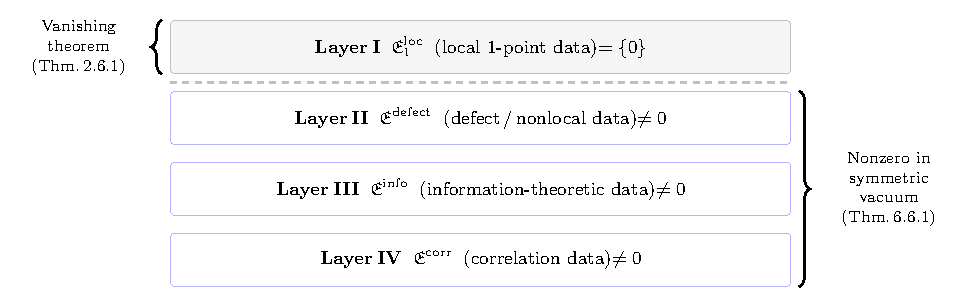
\includegraphics[width=0.75\columnwidth]{figures/fig1_four_layers_en.pdf}
\caption{The four-layer classification of vacuum data
  (Definition~\ref{def:four-layers}).
  Layer~I consists of local 1-point functions and is the domain
  of the vanishing theorem (Theorem~\ref{thm:vanishing}):
  $\mathfrak{E}_1^{\mathrm{loc}}(\rho_0)=\{0\}$.
  Layers~II--IV---defect, information-theoretic, and correlation
  data---are nonzero even in the source-free, symmetric vacuum
  (Theorem~\ref{thm:scope}).}
\label{fig:four-layers}
\end{figure}

% -----------------------------------------------------------------
\subsection{Scope of the vanishing theorem: refined
  statement}\label{subsec:6-6}

Under the classification above (see FIG.~\ref{fig:four-layers}),
we can finally clarify the scope
of the vanishing theorem of Section~\ref{sec:2}.

The following theorem is logically independent of the Unification
Theorem (Theorem~\ref{thm:unification}); it addresses the
\emph{scope} of the vanishing result rather than the deformation
response.

\begin{theorem}\label{thm:scope}
The Ward-identity-based vanishing proof of Section~\ref{sec:2}
applies only to~$\mathfrak{E}_1^{\mathrm{loc}}(\rho_0)$.
Therefore, for the source-free, symmetric vacuum~$\rho_0$
of the exact conformal
theory~$S_{\mathrm{CFT}}$,
\begin{equation}\label{eq:layer-I-vanish}
  \mathfrak{E}_1^{\mathrm{loc}}(\rho_0) = \{0\}
\end{equation}
(Theorem~\ref{thm:vanishing}).
On the other hand, in the canonical
example~$\AdS_5\times S^5/\N=4$~SYM, there exist observables
belonging to Layers~II--IV that are nonzero in~$\rho_0$:
\begin{equation}\label{eq:layers-nonzero}
  \langle W_\circ\rangle_0 \neq 0,\qquad
  \exists\,A,B\;\text{such that}\;
    I(A:B)_{\rho_0}\neq 0,\qquad
  \langle\mathcal{O}_\Delta(x)\,
    \mathcal{O}_\Delta(0)\rangle_0\neq 0\,.
\end{equation}
The vanishing theorem of Section~\ref{sec:2} therefore does not
extend to Layers~II--IV in general.
\end{theorem}

\begin{proof}
$\mathfrak{E}_1^{\mathrm{loc}}(\rho_0)=\{0\}$ follows from
Theorem~\ref{thm:vanishing}.
$\langle W_\circ\rangle_0\neq 0$ follows from
Proposition~\ref{prop:Wilson-nonzero}.
The existence of disjoint regions $A,B$ with
$I(A:B)_{\rho_0}\neq 0$ follows from the general properties
of mutual information in a CFT
vacuum~\cite{ref32,ref33}.
$\langle\mathcal{O}_\Delta(x)\,
\mathcal{O}_\Delta(0)\rangle_0\neq 0$ follows from the standard
properties of the 2-point function of a
CFT~\cite{ref5,ref13,ref14}.
\end{proof}

\begin{remark}\label{rem:scope-layer-specific}
This theorem makes explicit that the vanishing theorem of
Section~\ref{sec:2} is \textbf{specific to Layer~I}.
The symmetric vacuum of the exact conformal theory carries no
local intrinsic 1-point data, but it richly possesses the
capacity for probe response, quantum entanglement structure, and
multi-point relational structure.
What vanishes is ``the intrinsic 1-point data of the vacuum,''
not ``the physical content of the vacuum.''
\end{remark}

% -----------------------------------------------------------------
\subsection{Deepening the scope of the vanishing
  theorem}\label{subsec:6-7}

Theorem~\ref{thm:scope} deepens the results up to
Section~\ref{sec:5} in two senses.

First, it provides an answer to the open problem of
``the completeness of~$\Cex$'' that was left in
\S\ref{subsec:5-8}.
At least in the symmetric vacuum of the canonical
example~$\AdS_5\times S^5/\N=4$~SYM, there exist nonzero data
belonging to Layers~II--IV, so \textbf{$\Cex$ does not exhaust
the totality of nontrivial vacuum data}.

Second, this answer does not weaken the vanishing theorem of
Section~\ref{sec:2} but, on the contrary,
\textbf{sharply characterizes} its nature.
What the vanishing theorem captures is the specific class of
1-point vacuum data that is ``local, intrinsic, and of 1-point
type''; for that class, the vanishing is rigorous in the
symmetric vacuum of the exact conformal theory.
The fact that other classes of quantities do not vanish
clarifies the scope of the vanishing theorem and simultaneously
shows that \textbf{the concept of vacuum data itself is
multi-layered}.

In this sense, the vanishing theorem of this paper contains two
strata:
\begin{enumerate}
\item \textbf{First stratum:} the symmetric vacuum of the exact
  conformal theory carries no nontrivial vacuum data in the sense
  of Layer~I\@.
  In this sense, nonzero 1-point functions do not appear without
  deformation.
\item \textbf{Second stratum:} the vanishing theorem for
  Layer~I does not capture the totality of nontrivial vacuum data.
  The vacuum can carry nontrivial data in Layers~II--IV\@.
  In this sense, the definition of vacuum data via 1-point data
  is itself limited relative to the full scope of vacuum data.
\end{enumerate}

% -----------------------------------------------------------------
In Section~\ref{sec:7} we unify this four-layer classification
with the deformation theory of Section~\ref{sec:3}.

% =====================================================================
% §7 LAYER-RESOLVED RESPONSE
% =====================================================================
\section{Layer-resolved response to deformations}\label{sec:7}

In Section~\ref{sec:6} we classified observables into four layers
and showed that the vanishing theorem of Section~\ref{sec:2} is
a result specific to Layer~I, while in the canonical
example~$\AdS_5\times S^5/\N=4$~SYM Layers~II--IV carry nonzero
data even in the symmetric vacuum.
In this section we unify that four-layer classification with the
deformation theory of Section~\ref{sec:3} and systematically
describe how each layer changes under deformation.
We also reinterpret the effect of the~$\Lambda>0$ background
shown in Section~\ref{sec:4} in the language of the four-layer
structure.

This section has two tasks:
(1)~combine the four-layer notation of
Definition~\ref{def:four-layers} with each deformation of
Section~\ref{sec:3} and systematize the response of each layer
to deformation, and
(2)~connect the impact of the~$\Lambda>0$ background on this
four-layer structure with the results of Section~\ref{sec:4}.

% -----------------------------------------------------------------
\subsection{Definition of layer-resolved response quantities}%
  \label{subsec:7-1}

In Definition~\ref{def:vacuum-data-set} we introduced the
$\Cex$-relative vacuum data
$\mathfrak{E}_{\Cex}(\rho)$.
Definition~\ref{def:four-layers} decomposed this into four
layers:
\[
  \mathfrak{E}_1^{\mathrm{loc}}(\rho),\qquad
  \mathfrak{E}^{\mathrm{defect}}(\rho),\qquad
  \mathfrak{E}^{\mathrm{info}}(\rho),\qquad
  \mathfrak{E}^{\mathrm{corr}}(\rho)\,.
\]
In particular, Layer~I satisfies
$\mathfrak{E}_1^{\mathrm{loc}}(\rho)
=\mathfrak{E}_{\Cex}(\rho)$, i.e., it is the $\Cex$-relative
vacuum data defined in Section~\ref{sec:5} itself.
The four-layer classification of Section~\ref{sec:6}
systematically positions observables beyond the scope
of~$\Cex$---defect, information-theoretic, and
correlational---while keeping this data as its core.

By Theorem~\ref{thm:scope}, for the source-free, symmetric
vacuum~$\rho_0$ of the exact conformal theory,
Layer~I satisfies
$\mathfrak{E}_1^{\mathrm{loc}}(\rho_0)=\{0\}$,
while in the canonical
example~$\AdS_5\times S^5/\N=4$~SYM Layers~II--IV carry
nonzero data.
In Section~\ref{sec:3}, we showed that 1-point functions of
Layer~I can become nonzero under a
deformation~$\Delta S_{\mathrm{def}}$
(Theorem~\ref{thm:nonzero}).
However, that result concerns Layer~I only; how deformations
affect Layers~II--IV was not discussed.

To describe uniformly how each layer changes under deformation,
we introduce the following concept.

\begin{definition}\label{def:differential-response}
For the source-free, symmetric vacuum~$\rho_0$ of the exact
conformal theory and a deformed state~$\rho_{\mathrm{def}}$,
define the \textbf{differential response} of each layer as
follows.

\textbf{Layer~I (activation):}
\begin{equation}\label{eq:delta-I}
  \delta\mathfrak{E}_{\rho_0}^{\mathrm{loc}_1}%
    (\rho_{\mathrm{def}})
  := \bigl\{\,
    \langle\hat{\mathcal{O}}(x)\rangle_{\rho_{\mathrm{def}}}
    -\langle\hat{\mathcal{O}}(x)\rangle_{\rho_0}
    \;\big|\;
    \hat{\mathcal{O}}\in\Cex
  \bigr\}
  = \bigl\{\,
    \langle\hat{\mathcal{O}}(x)\rangle_{\rho_{\mathrm{def}}}
    \;\big|\;
    \hat{\mathcal{O}}\in\Cex
  \bigr\}\,.
\end{equation}
The second equality follows from
$\langle\hat{\mathcal{O}}(x)\rangle_{\rho_0}=0$
(Theorem~\ref{thm:vanishing}).
Thus the differential response of Layer~I represents activation
from zero.

For Layers~II--IV, since
$\mathfrak{E}^{(\alpha)}(\rho)$ is a family of individual
quantities listed in Definition~\ref{def:four-layers}, the
differential response is likewise defined as the family of
differences for each constituent:

\textbf{Layer~II (differential response):}
\begin{equation}\label{eq:delta-II}
  \delta\mathfrak{E}_{\rho_0}^{\mathrm{defect}}%
    (\rho_{\mathrm{def}})
  := \bigl\{\,
    \langle D_p(\Sigma_p)\rangle_{\rho_{\mathrm{def}}}
    -\langle D_p(\Sigma_p)\rangle_{\rho_0}
  \bigr\}\,.
\end{equation}

\textbf{Layer~III (differential response):}
\begin{multline}\label{eq:delta-III}
  \delta\mathfrak{E}_{\rho_0}^{\mathrm{info}}%
    (\rho_{\mathrm{def}})
  := \bigl\{\,
    S_A(\rho_{\mathrm{def}})-S_A(\rho_0),\;
    I(A{:}B)_{\rho_{\mathrm{def}}}-I(A{:}B)_{\rho_0},\\
    \langle K_A^{\rho_0}\rangle_{\rho_{\mathrm{def}}}
    -\langle K_A^{\rho_0}\rangle_{\rho_0},\;
    S(\rho_{\mathrm{def},A}\|\rho_{0,A}),\;\ldots
  \bigr\}\,.
\end{multline}
Here the relative entropy
$S(\rho_{\mathrm{def},A}\|\rho_{0,A})$ is not a difference
but is itself a response quantity relative to the reference
vacuum~$\rho_0$ (\S\ref{subsec:6-3}).

\textbf{Layer~IV (differential response):}
\begin{equation}\label{eq:delta-IV}
  \delta\mathfrak{E}_{\rho_0}^{\mathrm{corr}}%
    (\rho_{\mathrm{def}})
  := \bigl\{\,
    \langle\mathcal{O}_1(x_1)\cdots\mathcal{O}_n(x_n)
      \rangle_{\rho_{\mathrm{def}}}^c
    -\langle\mathcal{O}_1(x_1)\cdots\mathcal{O}_n(x_n)
      \rangle_{\rho_0}^c
  \bigr\}_{n\geq 2}\,.
\end{equation}

These are collectively written as
$\delta\mathfrak{E}_{\rho_0}^{(\alpha)}%
(\rho_{\mathrm{def}})$
($\alpha\in\{\mathrm{loc}_1,\,\mathrm{defect},\,
\mathrm{info},\,\mathrm{corr}\}$).
In each layer, the difference is computed by fixing the same
auxiliary data---the same defect~$D_p(\Sigma_p)$ for Layer~II,
the same subregion~$A$ (or pair~$A,B$) for Layer~III, the same
operators and insertion points for Layer~IV---and varying only
the state from $\rho_0$ to~$\rho_{\mathrm{def}}$.
\end{definition}

\begin{remark}\label{rem:diff-math}
As noted in Remark~\ref{rem:layers-not-sum}, the four layers do
not carry the same mathematical structure.
The ``differences'' defined here therefore have different
mathematical character in each layer:
\begin{itemize}
\item \textbf{Layer~II:} difference of operator expectation
  values---a well-defined numerical difference.
\item \textbf{Layer~III:} difference of nonlinear
  functionals (e.g.,
  $S_A(\rho_{\mathrm{def}})-S_A(\rho_0)$).
  By the entanglement first law
  (Proposition~\ref{prop:first-law}),
  linearization
  $\delta S_A\approx\delta\langle K_A\rangle$ is available
  near the reference vacuum.
\item \textbf{Layer~IV:} difference of multi-point
  functions---describing changes in the connected part.
\end{itemize}
Whether these differences take nontrivial values under
deformation is examined in the following subsections.
\end{remark}

% -----------------------------------------------------------------
\subsection{Relevant deformation and RG flow}\label{subsec:7-2}

We describe the relevant deformation
$\Delta S_{\mathrm{rel}}
=\int d^4x\,\lambda\,\mathcal{O}_\Delta(x)$
($\Delta<4$) of \S\ref{subsec:3-2} in the four layers.

\paragraph{Layer~I: activation.}
By Proposition~\ref{prop:relevant}, under a relevant deformation
scale invariance is explicitly broken and the vanishing of the
scalar 1-point function
$\langle\mathcal{O}_\Delta\rangle$ is no longer enforced.
By dimensional analysis,
\begin{equation}\label{eq:rel-scaling}
  \langle\mathcal{O}_\Delta\rangle
  \sim\lambda^{\Delta/(4-\Delta)}
\end{equation}
is expected.
Thus
$\delta\mathfrak{E}_{\rho_0}^{\mathrm{loc}_1}\neq\{0\}$
is permitted---this is the activation of Layer~I and a direct
consequence of the framework of Section~\ref{sec:3}.

\paragraph{Layer~II: response.}
In the conformal vacuum, the Wilson loop expectation value
$\langle W(C_R)\rangle$ is independent of the radius~$R$ by
conformal transformations and depends only on~$\lambda$
and~$N$ (\S\ref{subsec:6-2}).
A relevant deformation introduces an IR
scale~$\Lambda_{\mathrm{IR}}$, so
$\langle W(C_R)\rangle$ can depend on~$R\Lambda_{\mathrm{IR}}$.
This is shown directly by conformal perturbation theory.
Expanding the deformed Wilson loop to first order gives
\begin{equation}\label{eq:Wilson-CPT}
  \delta\log\langle W(C_R)\rangle
  = -\lambda\int d^4x\,
    \frac{\langle W(C_R)\,\mathcal{O}_\Delta(x)
      \rangle_{0,c}}
         {\langle W(C_R)\rangle_0}
    +O(\lambda^2)\,.
\end{equation}
The right-hand side is dominated by the defect CFT one-point
coefficient~$a_{\mathcal{O}}$~\cite{ref14,ref47}, and by
dimensional analysis
\begin{equation}\label{eq:Wilson-shift}
  \delta\log\langle W(C_R)\rangle
  \sim\lambda\,a_{\mathcal{O}}\,R^{4-\Delta}
\end{equation}
is derived~[Comp.~2].
When $a_{\mathcal{O}}\neq 0$, the Wilson loop exhibits an
$R$-dependence different from the conformal vacuum, and
$\delta\mathfrak{E}_{\rho_0}^{\mathrm{defect}}\neq 0$
can arise.

\paragraph{Layer~III: response.}
When a relevant deformation drives an RG flow, the entanglement
entropy tracks the change in degrees of freedom from UV to
IR~\cite{ref43}.
In holographic calculations, a domain-wall structure separates
the UV and IR regions, and the change in entanglement entropy
serves as a concrete indicator of UV/IR
mixing~\cite{ref43}.
This is understood within the framework of the $c$-theorem.
Hence
$\delta\mathfrak{E}_{\rho_0}^{\mathrm{info}}\neq 0$
can arise.

\paragraph{Layer~IV: response.}
When a relevant deformation flows to a gapped IR phase, the
connected 2-point function exhibits exponential decay
\begin{equation}\label{eq:gapped-corr}
  \langle\mathcal{O}(x)\,\mathcal{O}(0)\rangle^c
  \sim e^{-m|x|}\,.
\end{equation}
When it flows to another IR fixed point, the correlations are
reorganized into a power-law form with new scaling dimensions.
In either case, a qualitative change from the correlation
structure of the conformal vacuum occurs, and
$\delta\mathfrak{E}_{\rho_0}^{\mathrm{corr}}\neq 0$
can arise.

\begin{proposition}\label{prop:relevant-all-layers}
Under a relevant deformation
$\Delta S_{\mathrm{rel}}
=\int d^4x\,\lambda\,\mathcal{O}_\Delta$ ($\Delta<4$),
$\delta\mathfrak{E}_{\rho_0}^{(\alpha)}\neq 0$
is permitted in all four layers.
Layer~I undergoes activation; Layers~II--IV undergo nontrivial
responses.
\end{proposition}

\begin{proof}
Layer~I follows from
Proposition~\ref{prop:relevant}.
Layer~III is supported by holographic entanglement entropy
calculations of~\cite{ref43}.
Layer~IV follows from the standard result of finite correlation
length due to mass gap generation.
Layer~II is shown by conformal perturbation theory, which gives
the first-order shift
$\delta\log\langle W(C_R)\rangle
\sim\lambda\,R^{4-\Delta}$~[Comp.~2].
\end{proof}

\begin{remark}\label{rem:other-deformations}
The anomaly/CP-violation deformations of
\S\ref{subsec:3-6} and the time-dependent background of
\S\ref{subsec:3-7} were already treated in Section~\ref{sec:3}
as deformations of Layer~I\@.
The effect of these deformations on Layers~II--IV is not
systematically treated in this paper; however, in the language
of \S\ref{subsec:3-8} (bulk geometry deformation), all
deformations are understood on the bulk side as departures from
pure~$\AdS_5\times S^5$
(Proposition~\ref{prop:bulk-deformation}).
\end{remark}

% -----------------------------------------------------------------
\subsection{Finite temperature and finite density}%
  \label{subsec:7-3}

We describe the finite-temperature and finite-density
deformations of \S\ref{subsec:3-3}--\ref{subsec:3-4}
in the four layers.

\paragraph{Finite temperature.}
The deformation to finite temperature~$T>0$ is implemented as
compactification of Euclidean time
$\tau\sim\tau+\beta$ ($\beta=T^{-1}$).
On the AdS side it corresponds to the AdS-Schwarzschild black
brane~\cite{ref39}.

\emph{Layer~I: activation.}
By Proposition~\ref{prop:finite-T}, in the thermal state the
stress tensor 1-point function can become nonzero:
\begin{equation}\label{eq:thermal-Tmunu-finiteT}
  \langle T_{\mu\nu}\rangle_T
  = \mathrm{diag}(\varepsilon,p,p,p),\qquad
  \varepsilon = 3p\,.
\end{equation}
In the strong-coupling, large-$N$ limit
$\varepsilon\propto N^2 T^4$~\cite{ref4,ref39}.
Hence
$\delta\mathfrak{E}_{\rho_0}^{\mathrm{loc}_1}\neq\{0\}$
is permitted (activation).

\emph{Layer~II: response.}
At finite temperature the Wilson--Polyakov loop becomes the
natural defect quantity~\cite{ref40}.
Since $\N=4$~SYM is always in the deconfined phase, the
Polyakov loop is nonzero regardless of temperature.
The heavy-quark potential at finite temperature is computed from
the string worldsheet on the AdS-Schwarzschild
background~\cite{ref40,ref46} and shows finite-range
interactions, unlike the Coulomb-like potential in the conformal
vacuum.
Thus the Wilson loop expectation value acquires temperature
dependence, and
$\delta\mathfrak{E}_{\rho_0}^{\mathrm{defect}}\neq 0$
can arise.

\emph{Layer~III: response.}
At finite temperature, the entanglement entropy receives a
thermal entropy contribution~\cite{ref42}.
In the high-temperature limit the thermal entropy is dominant,
and the mutual information $I(A:B)$ contains both thermal and
quantum entanglement contributions~\cite{ref42}.
By the entanglement first law
$\delta S_A=\delta\langle K_A\rangle$
(Proposition~\ref{prop:first-law}), the change in entanglement
entropy for a ball region is directly linked to the change in the
stress tensor expectation value (Layer~I).
Hence
$\delta\mathfrak{E}_{\rho_0}^{\mathrm{info}}\neq 0$
can arise.

\emph{Layer~IV: response.}
At finite temperature, equal-time spatial correlators exhibit
exponential decay at large distances due to thermal
screening~\cite{ref39,ref46}.
The decay rate is determined by a thermal screening scale that
depends on the operator channel.
This is qualitatively different from the power-law correlations
of the conformal vacuum, and
$\delta\mathfrak{E}_{\rho_0}^{\mathrm{corr}}\neq 0$
can arise.

\begin{theorem}\label{thm:finiteT-layers}
Under the deformation to finite temperature ($T>0$), nontrivial
responses can arise in all four layers:
\begin{equation}\label{eq:finiteT-response}
  \delta\mathfrak{E}_{\rho_0}^{(\alpha)}(\rho_T)\neq 0
  \;\;\text{is permitted}
  \quad
  (\alpha\in\{\mathrm{loc}_1,\,\mathrm{defect},\,
    \mathrm{info},\,\mathrm{corr}\})\,.
\end{equation}
\end{theorem}

\begin{proof}
Layer~I follows from
Proposition~\ref{prop:finite-T}.
Layer~II from the finite-temperature Wilson--Polyakov loop
computation of~\cite{ref40}.
Layer~III from the finite-temperature holographic entanglement
entropy results of~\cite{ref42}.
Layer~IV from the standard thermal screening results
of~\cite{ref39}.
\end{proof}

\paragraph{Finite density.}
A finite chemical potential $\mu\neq 0$ is implemented as the
introduction of a source for the time component of the
current~$J_\mu^A$ (\S\ref{subsec:3-4}).
On the AdS side it corresponds to a charged black brane
background~\cite{ref9,ref10,ref11}.

\emph{Layer~I: activation.}
By Proposition~\ref{prop:finite-mu},
$\langle J_0^A\rangle_\mu\neq 0$ is permitted (activation).

\emph{Layer~II: response.}
The Wilson loop at finite chemical potential is computed from
the string worldsheet on a charged black brane
background~\cite{ref44} and yields a heavy-quark potential
differing from the conformal vacuum result.
Hence
$\delta\mathfrak{E}_{\rho_0}^{\mathrm{defect}}\neq 0$
can arise.

\emph{Layer~III: response.}
The change in entanglement entropy at finite density can be
directly evaluated via the entanglement first law
(Proposition~\ref{prop:first-law}).
For a ball region~$B_R$,
\begin{equation}\label{eq:EE-density}
  \Delta S_{B_R}
  = \frac{8\pi^2}{15}\,R^4\,\Delta\varepsilon(\mu)\,,
\end{equation}
where
$\Delta\varepsilon(\mu)=\varepsilon(\mu)-\varepsilon(0)$
is the increase in energy density due to the chemical
potential~[Comp.~3].
From the thermodynamics of the AdS-Reissner--Nordstr\"om
background,
$\Delta\varepsilon\propto Q^2 r_h^4>0$, so
$\Delta S_{B_R}\neq 0$.
Furthermore, in holographic calculations the shape of the
Ryu--Takayanagi surface differs between AdS-RN and pure
AdS~\cite{ref42}, as confirmed
numerically~[Comp.~3].
The relative entropy
$S(\rho_{\mu,A}\|\rho_{0,A})>0$ also provides an independent
signal.
Hence
$\delta\mathfrak{E}_{\rho_0}^{\mathrm{info}}\neq 0$
can arise.

\emph{Layer~IV: response.}
Finite density directly affects the screening length of
correlation functions.
Analysis of scalar fluctuations on the AdS-RN background shows
that the screening length~$\xi$ depends on the chemical
potential~$\mu$~[Comp.~4].
In particular, in the extremal limit ($T=0$, $\mu\neq 0$)
screening arises solely from finite density without any thermal
contribution, producing a structure qualitatively different from
the power-law correlations of the conformal vacuum.
The quasinormal mode frequencies also shift with~$\mu$,
modifying the analytic structure of the correlator.
Hence
$\delta\mathfrak{E}_{\rho_0}^{\mathrm{corr}}\neq 0$
can arise.

\begin{proposition}\label{prop:density-all-layers}
Under the deformation to finite density ($\mu\neq 0$),
nontrivial responses can arise in all four layers:
Layer~I (charge density activation),
Layer~II (Wilson loop change~\cite{ref44}),
Layer~III (entanglement first law giving
$\Delta S_{B_R}\neq 0$~[Comp.~3]),
Layer~IV (screening length $\mu$-dependence~[Comp.~4]).
\end{proposition}

\begin{proof}
Layer~I from
Proposition~\ref{prop:finite-mu}.
Layer~II from the Wilson loop computation at finite chemical
potential of~\cite{ref44}.
Layer~III from the combination of the entanglement first law
and AdS-RN thermodynamics, giving
$\Delta S_{B_R}=(8\pi^2/15)\,R^4\,\Delta\varepsilon(\mu)
\neq 0$~\cite{ref42}; see also~[Comp.~3].
Layer~IV from the analysis of scalar fluctuations on the
charged black brane, showing that the screening length depends
on~$\mu$~[Comp.~4].
\end{proof}

% -----------------------------------------------------------------
\subsection{Vacuum selection and the Coulomb branch}%
  \label{subsec:7-4}

We describe the vacuum selection to the Coulomb branch
of \S\ref{subsec:3-5} in the four layers.

On the Coulomb branch of~$\N=4$~SYM, the adjoint
scalar~$\Phi^I$ acquires nonzero eigenvalues and the gauge
group $SU(N)$ is spontaneously broken to, e.g.,
$SU(N-1)\times U(1)$~\cite{ref4,ref6,ref7}.
On the AdS side, this corresponds to separating a probe
D3-brane into the bulk.

\emph{Layer~I: activation.}
By Proposition~\ref{prop:Coulomb}, on the Coulomb branch
gauge-invariant Coulomb-branch operators such as chiral
primaries
$\langle\mathrm{Tr}(\Phi^{(I_1}\cdots\Phi^{I_k)})
\rangle\neq 0$
are permitted.
Holographic calculations~\cite{ref45} reproduce this
quantitatively from the supergravity solution on the
Coulomb-branch geometry.
This is an activation of Layer~I, tied to the spontaneous
breaking of conformal symmetry.

\emph{Layer~II: response.}
On the Coulomb branch, the VEV introduces a new scale~$v$,
so the Wilson loop and heavy-probe potential are deformed from
the conformal vacuum results.
Holographically, this appears as a change in the minimal
worldsheet on the bulk geometry reflecting the separated
D3-brane~\cite{ref28}.
The detailed asymptotics depend on the representation of the
Wilson loop and the choice of Coulomb-branch vacuum; here we
do not assert a universal asymptotic law but note that a change
from the conformal vacuum is present:
$\delta\mathfrak{E}_{\rho_0}^{\mathrm{defect}}\neq 0$
can arise.

\emph{Layer~III: response.}
The entanglement entropy on the Coulomb branch has been directly
evaluated by holographic probe D3-brane
calculations~\cite{ref41}.
For $SU(N)\to SU(N-1)\times U(1)$, the entanglement entropy
decreases monotonically relative to the conformal vacuum,
consistent with the $a$-theorem~\cite{ref41}.
Hence
$\delta\mathfrak{E}_{\rho_0}^{\mathrm{info}}\neq 0$
can arise.

\emph{Layer~IV: response.}
On the Coulomb branch, correlation functions are reorganized
into Yukawa-type contributions from massive W-bosons and
long-range contributions from the residual massless Abelian
sector.
A structure different from the simple power-law correlations
$\sim|x|^{-2\Delta}$ of the conformal vacuum emerges, and
$\delta\mathfrak{E}_{\rho_0}^{\mathrm{corr}}\neq 0$
can arise.

\begin{theorem}\label{thm:Coulomb-layers}
Under vacuum selection to the Coulomb branch, nontrivial
responses can arise in all four layers:
\begin{equation}\label{eq:Coulomb-response}
  \delta\mathfrak{E}_{\rho_0}^{(\alpha)}%
    (\rho_{\mathrm{Coulomb}})\neq 0
  \;\;\text{is permitted}
  \quad
  (\alpha\in\{\mathrm{loc}_1,\,\mathrm{defect},\,
    \mathrm{info},\,\mathrm{corr}\})\,.
\end{equation}
\end{theorem}

\begin{proof}
Layer~I from
Proposition~\ref{prop:Coulomb}
(with quantitative support from the holographic computation
of~\cite{ref45}).
Layer~II from the deformation of bulk geometry and the change in
the minimal worldsheet due to the VEV~\cite{ref28}.
Layer~III from the holographic entanglement entropy computation
on the Coulomb branch of~\cite{ref41}.
Layer~IV from the reorganization of the correlation structure
into massive W-boson and residual massless sectors.
\end{proof}

\begin{remark}\label{rem:Coulomb-Wilson}
In Proposition~\ref{prop:Wilson-nonzero} we showed that the
Wilson loop expectation value is nonzero even in the conformal
vacuum ($\langle W_\circ\rangle_0>0$).
The change on the Coulomb branch is understood not as a change
in this nonzero value itself but as a qualitative change in the
contour dependence of the Wilson loop---i.e., in the nature of
the heavy-quark potential.
\end{remark}

% -----------------------------------------------------------------
\subsection{Four-layer structure of the
  \texorpdfstring{$\Lambda>0$}{Lambda>0}
  background}\label{subsec:7-5}

We reinterpret the results of Section~\ref{sec:4} in the
language of the four-layer structure.
In Section~\ref{sec:4} we showed as Proposition~\ref{thm:lambda}
that the~$\Lambda>0$ background does not preserve the assumptions
supporting the vanishing theorem of Section~\ref{sec:2}.
The purpose here is to clarify how this failure manifests in each
layer of the four-layer structure.

The main breakdowns of assumptions shown in Section~\ref{sec:4}
are:
(i)~loss of the flat-space implementation of scale invariance
(introduction of the IR scale by~$H$),
(ii)~absence of the source/response dictionary on a timelike
boundary,
(iii)~loss of the cold-vacuum interpretation (Gibbons--Hawking
temperature),
(iv)~instability of the local implementation of global symmetry.
Below we organize how these affect each layer.

\emph{Layer~I: activation.}
As shown in Propositions~\ref{prop:GH-thermal}
and~\ref{prop:IR-scale}, on a de~Sitter background the
Gibbons--Hawking temperature
$T_{\dS}=H/(2\pi)$ defines a thermal state for the local
observer, and the Hubble rate~$H$ obstructs the vanishing via the
scale Ward identity as an IR scale.
Hence
$\delta\mathfrak{E}_{\rho_0}^{\mathrm{loc}_1}\neq\{0\}$
is permitted.
A well-known constructive realization is the trace anomaly:
on a curved background, the renormalized stress tensor acquires
a nonzero trace
$\langle T^\mu{}_\mu\rangle
  = (a/16\pi^2)\,E_4 + (c/16\pi^2)\,C_{\mu\nu\rho\sigma}^2$,
where $E_4$ is the Euler density and
$C_{\mu\nu\rho\sigma}$ the Weyl tensor~\cite{ref23}.
On de~Sitter, $E_4 = 24 H^4\neq 0$, so
$\langle T^\mu{}_\mu\rangle\neq 0$ and hence
$\langle T_{\mu\nu}\rangle\neq 0$---an explicit nonzero
Layer~I 1-point datum.
This is understood as a geometric implementation of the finite-temperature response of \S\ref{subsec:7-3}: in the
finite-temperature deformation the thermal state was introduced
by hand, whereas on the~$\Lambda>0$ background the existence of
the horizon automatically imposes a thermal state on the local
observer~\cite{ref15}.

\emph{Layer~II: prospect.}
By Proposition~\ref{prop:no-boundary-functional}, the
AdS/CFT-type source/response dictionary on a timelike boundary
is not available in standard form on de~Sitter.
This dictionary was the foundation for holographic computation
of defect quantities---in particular the Wilson
loop~(\S\ref{subsec:6-2}).
In the dS/CFT framework~\cite{ref18}, the formulation of defect
quantities is underdeveloped, and a systematic description of
the impact of~$\Lambda>0$ on Layer~II is limited within the
current theoretical framework.

\emph{Layer~III: response.}
As shown in Section~\ref{sec:4}, the cosmological horizon of
de~Sitter carries a Gibbons--Hawking entropy
\begin{equation}\label{eq:dS-entropy}
  S_{\dS} = \frac{A_{\mathrm{hor}}}{4G_N}
\end{equation}
\cite{ref15}
(for~$dS_4$, $A_{\mathrm{hor}}=4\pi L_{\dS}^2$ gives
$S_{\dS}=\pi L_{\dS}^2/G_N$).
This is naturally understood as a quantity belonging to the
information-theoretic/thermodynamic data of Layer~III\@.
Although it is not identical to the subsystem entanglement
entropy of the conformal vacuum, in the sense that
coarse-graining by the horizon yields a finite
information-theoretic contribution, it bears a structural
similarity to the Layer~III response at finite temperature
in \S\ref{subsec:7-3}.
Moreover, the Gibbons--Hawking thermal state at
$T_{\dS}=H/(2\pi)$ implies a nonzero von~Neumann entropy for
QFT subsystems---a genuine Layer~III quantity independent of
the gravitational horizon entropy~$S_{\dS}$.
Hence
$\delta\mathfrak{E}_{\rho_0}^{\mathrm{info}}\neq 0$
can arise.

\emph{Layer~IV: response.}
The causal structure of de~Sitter restricts the region
accessible to a local observer by the static patch
horizon~\cite{ref17,ref20,ref21}.
This restriction functions as an IR cutoff on correlation
functions.
Even without presupposing a complete boundary dictionary of
dS/CFT, within the QFT-on-de~Sitter framework correlation
functions with explicit~$\Lambda>0$ dependence are calculable.
For example, the scalar 2-point function in the Bunch--Davies
vacuum~\cite{ref22,ref23} is given as a function of the
de~Sitter-invariant distance~$Z$:
\begin{equation}\label{eq:dS-2pt}
  G^+(Z) \propto
  {}_2F_1\!\Bigl(\Delta_+,\Delta_-;\,2;\,
    \frac{1+Z}{2}\Bigr),
  \qquad
  \Delta_\pm = \frac{3}{2}\pm
    \sqrt{\frac{9}{4}-\frac{m^2}{H^2}}\,,
\end{equation}
which has explicit dependence on the Hubble rate~$H$.
This is qualitatively different from the power-law
correlations~$\sim|x|^{-2\Delta}$ of flat-space CFT, and
$\delta\mathfrak{E}_{\rho_0}^{\mathrm{corr}}\neq 0$
can arise.
However, this description does not imply a complete boundary
dictionary of full dS quantum gravity.

\begin{proposition}\label{prop:Lambda-layers}
$\Delta S_{\Lambda>0}$ (Definition~\ref{def:Lambda-deformation})
can produce nontrivial responses in at least Layer~I (possibility
of 1-point data activation via the local thermal state),
Layer~III (horizon entropy), and Layer~IV ($H$-dependence of
correlation functions in the QFT-on-de~Sitter
framework~\cite{ref22,ref23}).
The impact on Layer~II is limited within the current framework
because the definition of observables is framework-dependent.
\end{proposition}

\begin{proof}
Layer~I: by Proposition~\ref{prop:GH-thermal}, the static patch
observer experiences a thermal state at
$T_{\dS}=H/(2\pi)$~\cite{ref15}.
This is structurally equivalent to Layer~I of the
finite-temperature response in
Theorem~\ref{thm:finiteT-layers}.
In addition, the trace anomaly on de~Sitter gives
$\langle T^\mu{}_\mu\rangle\neq 0$~\cite{ref23},
providing a constructive Layer~I realization.
Layer~III: the horizon entropy~$S_{\dS}$ provides finite
information-theoretic data~\cite{ref15} and constitutes an
information-theoretic response analogous to the thermal entropy
of \S\ref{subsec:7-3}.
Layer~IV: within the QFT-on-de~Sitter framework the
Bunch--Davies 2-point function depends explicitly
on~$H$~\cite{ref22,ref23}, giving a structure qualitatively
different from flat-space CFT power-law correlations.
Layer~II: by Proposition~\ref{prop:no-boundary-functional},
the absence of the source/response dictionary obstructs the
holographic formulation of defect
quantities~\cite{ref16,ref17,ref18,ref19,ref20,ref21}.
\end{proof}

\begin{remark}\label{rem:Lambda-layers-new}
Proposition~\ref{thm:lambda} asserts that the vanishing theorem of
Section~\ref{sec:2} does not hold for~$\Lambda>0$, but its
discussion was centered on Layer~I (scalar 1-point function,
stress tensor).
The new contribution of this subsection is to position this
failure within the four-layer structure and to show:
(i)~for Layers~I and~III, it can be concretely understood as a
geometric implementation of the finite-temperature response,
(ii)~for Layer~IV, the change in correlation structure is
describable within the QFT-on-de~Sitter framework without
presupposing a complete boundary dictionary of dS/CFT, and
(iii)~for Layer~II, systematic description is limited because
the definition of observables is framework-dependent.
\end{remark}

% -----------------------------------------------------------------
\subsection{Layer-resolved response theorem}\label{subsec:7-6}

Integrating the results of \S\ref{subsec:7-2}--\ref{subsec:7-5},
we state a four-layer extension of
Theorem~\ref{thm:nonzero} and the unification theorem
(Theorem~\ref{thm:unification}).
Theorem~\ref{thm:nonzero} was a claim limited to the 1-point
functions belonging to~$\Cex$---i.e., Layer~I\@.
Theorem~\ref{thm:unification} unified it with the vanishing
theorem of Section~\ref{sec:2} and the~$\Lambda>0$ results of
Section~\ref{sec:4}.
The following theorem asserts that the same deformations
systematically affect Layers~II--IV as well.

\begin{theorem}[Layer-resolved response theorem]%
  \label{thm:layer-response}
For the source-free, symmetric vacuum~$\rho_0$ of the exact
conformal theory~$S_{\mathrm{CFT}}$:

\textbf{(1)}
$\mathfrak{E}_1^{\mathrm{loc}}(\rho_0)=\{0\}$
(Theorem~\ref{thm:vanishing}).
In the canonical
example~$\AdS_5\times S^5/\N=4$~SYM,
$\mathfrak{E}^{\mathrm{defect}}(\rho_0)$,
$\mathfrak{E}^{\mathrm{info}}(\rho_0)$, and
$\mathfrak{E}^{\mathrm{corr}}(\rho_0)$ contain nonzero examples
(Theorem~\ref{thm:scope}).

\textbf{(2)} Under a deformation
$\Delta S_{\mathrm{def}}$:
\begin{itemize}
\item Layer~I:
  $\mathfrak{E}_1^{\mathrm{loc}}(\rho_{\mathrm{def}})
  \neq\{0\}$ is permitted
  (Theorem~\ref{thm:nonzero}; holds for general deformations).
\end{itemize}
For the representative deformations treated in
\S\ref{subsec:7-2}--\ref{subsec:7-5}, furthermore:
\begin{itemize}
\item Layer~II:
  $\delta\mathfrak{E}_{\rho_0}^{\mathrm{defect}}%
  (\rho_{\mathrm{def}})\neq 0$ can arise.
\item Layer~III:
  $\delta\mathfrak{E}_{\rho_0}^{\mathrm{info}}%
  (\rho_{\mathrm{def}})\neq 0$ can arise.
\item Layer~IV:
  $\delta\mathfrak{E}_{\rho_0}^{\mathrm{corr}}%
  (\rho_{\mathrm{def}})\neq 0$ can arise.
\end{itemize}

\textbf{(3)} The~$\Lambda>0$ background geometrically implements
part~(2).
Nontrivial responses can arise in Layers~I, III, and~IV
(Proposition~\ref{prop:Lambda-layers}).
The impact on Layer~II is limited in systematic description
because the definition of observables is framework-dependent.
\end{theorem}

\begin{proof}
(1) follows from Theorem~\ref{thm:vanishing} and
Theorem~\ref{thm:scope}.

(2) For Layer~I, follows from Theorem~\ref{thm:nonzero}
because the deformation breaks at least one of the assumptions
supporting the vanishing theorem of Section~\ref{sec:2}.
For Layers~II--IV, confirmed by concrete examples in
\S\ref{subsec:7-2}--\ref{subsec:7-4}:
finite temperature
(Theorem~\ref{thm:finiteT-layers}),
Coulomb branch
(Theorem~\ref{thm:Coulomb-layers}),
relevant deformation
(Proposition~\ref{prop:relevant-all-layers}),
and finite density
(Proposition~\ref{prop:density-all-layers})
all exhibit nontrivial responses in all four layers.
Layer~II of the relevant deformation is supported by an
explicit conformal perturbation theory
calculation~[Comp.~2],
Layer~III of finite density by the entanglement first
law~[Comp.~3],
and Layer~IV by correlator analysis on the charged black
brane~[Comp.~4].

(3) follows from Proposition~\ref{prop:Lambda-layers}.
\end{proof}

\begin{remark}\label{rem:layer-response-asymmetry}
The claims of Theorem~\ref{thm:layer-response}(2) regarding
Layers~II--IV differ in theoretical completeness from the
Layer~I case.
The activation of Layer~I is derived deductively from
Theorem~\ref{thm:nonzero}: if the assumptions of the vanishing
theorem are broken, nonvanishing of the 1-point function is
permitted.

For the response of Layers~II--IV, on the other hand, no such
general vanishing/nonvanishing dichotomy exists.
In the canonical example, Layers~II--IV are already nonzero in
the reference vacuum (Theorem~\ref{thm:scope}); the question is
whether nontrivial \emph{changes} arise under deformation.
What was confirmed in
\S\ref{subsec:7-2}--\ref{subsec:7-4}
is the inductive fact that, for each concrete deformation
example, the response in each corresponding layer is shown to
be nontrivial by explicit calculations: conformal perturbation
theory~[Comp.~2], holographic entanglement
entropy~[Comp.~3], and correlator analysis on a charged
black brane~[Comp.~4].
Of the 20~cells in the matrix, 19 have now reached
$\checkmark$ (or $\checkmark^*$); the only remaining
$\triangle$ is~$\Lambda>0\times$Layer~II, which stems not from
a lack of computational technique but from the fact that the
definition of observables is framework-dependent.

This asymmetry reflects that the theoretical development of the
four-layer structure is not as complete as that of Layer~I\@.
For Layer~I there is a clear structure: a rigorous vanishing
theorem based on Ward identities and its negation.
The construction of an analogous general theory for
Layers~II--IV---for example, a necessary and sufficient
condition for the response of a defect quantity to be nontrivial
under deformation---is an important future task.
\end{remark}

\paragraph{``Deformation $\times$ layer'' matrix.}
As a corollary of Theorem~\ref{thm:layer-response}, the results
of
\S\ref{subsec:7-2}--\ref{subsec:7-5}
are summarized in TABLE~\ref{tab:matrix}.

\begin{table}[h]
\caption{Deformation $\times$ layer response matrix.
  $\checkmark$ = nontrivial response supported by literature
  or explicit computation;
  $\checkmark^*$ = describable within the QFT-on-de~Sitter
  framework (does not imply a full dS quantum gravity
  boundary dictionary);
  $\triangle$ = systematic description limited because the
  definition of observables is
  framework-dependent.
  The Layer~I vanishing and scope results hold at all~$N$
  and~$\lambda$.
  The Layer~II--IV entries are supported at large~$N$ and
  strong coupling via holographic computations.}\label{tab:matrix}
\begin{ruledtabular}
\begin{tabular}{lcccc}
 & Layer~I & Layer~II & Layer~III & Layer~IV \\
 & $\mathfrak{E}_1^{\mathrm{loc}}$
 & $\mathfrak{E}^{\mathrm{defect}}$
 & $\mathfrak{E}^{\mathrm{info}}$
 & $\mathfrak{E}^{\mathrm{corr}}$\\
\colrule
Relevant def.\ (\S\ref{subsec:7-2})
  & $\checkmark$ & $\checkmark$ [Comp.~2]
  & $\checkmark$ & $\checkmark$ \\
Finite $T$ (\S\ref{subsec:7-3})
  & $\checkmark$ & $\checkmark$
  & $\checkmark$ & $\checkmark$ \\
Finite $\mu$ (\S\ref{subsec:7-3})
  & $\checkmark$ & $\checkmark$
  & $\checkmark$ [Comp.~3] & $\checkmark$ [Comp.~4] \\
Coulomb branch (\S\ref{subsec:7-4})
  & $\checkmark$ & $\checkmark$
  & $\checkmark$ & $\checkmark$ \\
$\Lambda>0$ (\S\ref{subsec:7-5})
  & $\checkmark$ & $\triangle$
  & $\checkmark$ & $\checkmark^*$ \\
\end{tabular}
\end{ruledtabular}
\end{table}

Layer~I is~$\checkmark$ for all deformations, which is a
deductive consequence of Theorem~\ref{thm:nonzero}.
All four layers are~$\checkmark$ for the relevant deformation,
finite temperature, finite density, and Coulomb branch.
The only~$\triangle$ is
$\Lambda>0\times$Layer~II (defect), which stems not from a
computational limitation but from the non-uniqueness of the
definition of defect observables on a~$\Lambda>0$ background.

% -----------------------------------------------------------------
\subsection{Outlook}\label{subsec:7-7}

We position the results of this section within the framework of
the two limitations identified in \S\ref{subsec:6-7}.

In \S\ref{subsec:6-7} we showed that the vanishing theorem and
the deformation principle of this paper contain two limitations:
(1)~in the sense of Layer~I, the symmetric vacuum of the exact
conformal theory carries no nontrivial vacuum data, and
(2)~the vanishing theorem for Layer~I does not capture the
totality of nontrivial vacuum data.
Section~\ref{sec:7} has deepened this structure as follows.

\begin{itemize}
\item \textbf{Refinement of the first limitation:}
  the activation of Layer~I is completely described by
  Theorem~\ref{thm:nonzero}.
  Section~\ref{sec:7} additionally showed that the same
  deformations produce systematic responses in Layers~II--IV as
  well.
  That is, the effect of deformation does not remain confined
  to the activation of Layer~I but can propagate across all four
  layers (Theorem~\ref{thm:layer-response}).

\item \textbf{Structuring of the second limitation:}
  Section~\ref{sec:6} merely showed that Layers~II--IV are
  nonzero in the symmetric vacuum of the canonical example.
  Section~\ref{sec:7} formulated the changes in Layers~II--IV
  under deformation as ``differential responses''
  (Definition~\ref{def:differential-response}) and described
  their behavior for each concrete example.
\end{itemize}

\paragraph{Remaining tasks.}
As Theorem~\ref{thm:layer-response} and
Remark~\ref{rem:layer-response-asymmetry} make explicit, the
following directions are important future tasks:
\begin{enumerate}
\item \textbf{General theorem for Layers~II--IV:}
  currently the claims rest on inductive evidence from concrete
  examples.
  Establishing a deductive structure analogous to Layer~I---general conditions under which the response of
  Layers~II--IV to deformation is nontrivial---is needed.
\item \textbf{Systematic theory for the defect layer
  at~$\Lambda>0$:}
  as the sole~$\triangle$ cell in the matrix
  ($\Lambda>0\times$Layer~II) indicates, the definition of defect
  observables on a~$\Lambda>0$ background is
  framework-dependent, and a systematic theory is underdeveloped.
  For Layer~IV, it has been shown
  (Proposition~\ref{prop:Lambda-layers}) that description is
  possible within the QFT-on-de~Sitter framework, but a complete
  extension to the defect layer awaits progress in the
  formulation of dS/CFT\@.
\item \textbf{Completeness problem for an extended operator
  family beyond~$\Cex$:}
  the completeness of the operator family~$\Cex$ raised in
  \S\ref{subsec:5-8} and \S\ref{subsec:6-7} has been clarified
  in scope by the introduction of the four-layer structure but
  remains unresolved.
  Whether the totality of the four layers exhausts all nontrivial
  vacuum data is still an open problem.
\end{enumerate}

In this section we unified the four-layer classification of
Section~\ref{sec:6} with the deformations of
Section~\ref{sec:3} and systematically described how each layer
changes under deformation.
The layer-resolved response theorem
(Theorem~\ref{thm:layer-response}) is positioned as a four-layer
extension of Theorem~\ref{thm:nonzero} and shows that the
response of vacuum data to deformation propagates beyond the
activation of Layer~I to all four layers.
At the same time, as Remark~\ref{rem:layer-response-asymmetry}
frankly acknowledged, the theoretical description of
Layers~II--IV is not as complete as that of Layer~I\@.
This asymmetry itself reflects the claim of this paper:
the concept of 1-point vacuum data is multi-layered, and
the theoretical maturity of each layer differs.

% =====================================================================
% §8 CONCLUSION
% =====================================================================
\section{Conclusion}\label{sec:8}

In Section~\ref{sec:5} we assembled the
vanishing theorem and the possibility of nonvanishing into the
unification theorem (Theorem~\ref{thm:unification}).
In Section~\ref{sec:6} we clarified the scope of the vanishing
theorem through the four-layer classification
(Definition~\ref{def:four-layers}).
In Section~\ref{sec:7} we established the layer-resolved response
theorem (Theorem~\ref{thm:layer-response}).
In this section we condense the results of
Sections~\ref{sec:1}--\ref{sec:7}, making explicit the final
claims, the logical structure of falsification, and the scope
and limitations of this paper.

% -----------------------------------------------------------------
\subsection{What has been achieved}\label{subsec:8-1}

The argument of this paper consists of three stages.

\textbf{Stage~1 (\S\ref{sec:2}--\ref{sec:5}).}
We showed that the 1-point function of every element of the
adopted operator family~$\Cex$ vanishes in the source-free,
symmetric vacuum of the exact conformal
theory~$S_{\mathrm{CFT}}$
(Theorem~\ref{thm:vanishing}).
We systematized that these 1-point functions can become nonzero
under a deformation~$\Delta S_{\mathrm{def}}$
(Theorem~\ref{thm:nonzero}).
We showed that a~$\Lambda>0$ background can be regarded as a
geometric implementation of such a deformation
(Proposition~\ref{thm:lambda}).
These were assembled into the unification theorem
(Theorem~\ref{thm:unification}).

\textbf{Stage~2 (\S\ref{sec:6}).}
We addressed the completeness problem for the operator
family~$\Cex$ left in \S\ref{subsec:5-8}, examining
observables not belonging to~$\Cex$---defect, information-theoretic,
and higher-point correlation functions.
We classified observables into four layers
(Definition~\ref{def:four-layers}) and clarified that the
vanishing theorem of Section~\ref{sec:2} is a result specific
to Layer~I (Theorem~\ref{thm:scope}).

\textbf{Stage~3 (\S\ref{sec:7}).}
We unified the four-layer classification with the deformation
theory and systematically described how each layer changes under
deformation.
We established the layer-resolved response theorem
(Theorem~\ref{thm:layer-response}) and supported nontrivial
responses in 19 out of 20~cells of the
``deformation~$\times$~layer'' matrix.

% -----------------------------------------------------------------
\subsection{Final claims}\label{subsec:8-2}

In \S\ref{subsec:5-9} we presented the conclusion limited to
$\Cex$-relative 1-point data as two boxed propositions.
With the results of Sections~\ref{sec:6}--\ref{sec:7}, this
conclusion is extended to the entire four-layer structure.

\begin{proposition}\label{prop:final-claim}
\textbf{(1)} For the source-free, symmetric vacuum~$\rho_0$
of the exact conformal theory~$S_{\mathrm{CFT}}$,
\begin{equation}\label{eq:final-vanish}
  \mathfrak{E}_1^{\mathrm{loc}}(\rho_0) = \{0\}
\end{equation}
(Theorem~\ref{thm:vanishing}).
In the canonical
example~$\AdS_5\times S^5/\N=4$~SYM, there exist observables
belonging to Layers~II--IV that are nonzero
in~$\rho_0$ (Theorem~\ref{thm:scope}).

\textbf{(2)} Under a deformation
$\Delta S_{\mathrm{def}}$, in addition to the activation of
Layer~I (Theorem~\ref{thm:nonzero}), systematic responses
can also arise in Layers~II--IV for the representative
deformations treated in
\S\ref{subsec:7-2}--\ref{subsec:7-5}
(Theorem~\ref{thm:layer-response}).

\textbf{(3)} Of the 20~cells formed by the representative
deformations (relevant deformation, finite temperature, finite
density, Coulomb branch, $\Lambda>0$) and the four layers,
19~are supported by literature evidence, explicit computation,
or the QFT-on-de~Sitter framework.
The only unconfirmed cell is
$\Lambda>0\times$Layer~II (defect), which stems from the fact
that the definition of observables is framework-dependent.
\end{proposition}

\begin{proof}
The first half of~(1) follows from
Theorem~\ref{thm:vanishing}, the second half from
Theorem~\ref{thm:scope}.
(2) follows from Theorem~\ref{thm:layer-response}.
(3) follows from
Proposition~\ref{prop:relevant-all-layers},
Theorem~\ref{thm:finiteT-layers},
Proposition~\ref{prop:density-all-layers},
Theorem~\ref{thm:Coulomb-layers}, and
Proposition~\ref{prop:Lambda-layers}
of \S\ref{subsec:7-2}--\ref{subsec:7-5}.
\end{proof}

\begin{remark}\label{rem:extension-from-5}
The two boxed propositions of \S\ref{subsec:5-9} were limited
to Layer~I\@.
Proposition~\ref{prop:final-claim} extends them to the full
four-layer structure.
The content of the extension is summarized as follows:
\begin{equation}\label{eq:final-box1}
  \fbox{\parbox{0.88\columnwidth}{%
    In the symmetric vacuum of the exact conformal theory,
    $\mathfrak{E}_1^{\mathrm{loc}}(\rho_0)=\{0\}$;
    the scope of the vanishing theorem is limited to
    Layer~I.}}
\end{equation}
\begin{equation}\label{eq:final-box2}
  \fbox{\parbox{0.88\columnwidth}{%
    Under a deformation~$\Delta S_{\mathrm{def}}$,
    in addition to the activation of Layer~I,
    systematic responses can arise in Layers~II--IV.}}
\end{equation}
Whereas \S\ref{subsec:5-9} stated the vanishing and the
possibility of nonvanishing for $\Cex$-relative 1-point data,
the above states the results for the entire four-layer structure
of vacuum data.
\end{remark}

% -----------------------------------------------------------------
\subsection{Falsification structure}\label{subsec:8-3}

To overturn the main theorems of this paper, logically one of the
following two routes is necessary.

\textbf{(1) Finding a mathematical error in the proofs.}
If any of the proof steps of
Theorems~\ref{thm:vanishing}, \ref{thm:nonzero},
\ref{thm:unification}, \ref{thm:scope},
or~\ref{thm:layer-response}
contains a mathematically incorrect inference.
Concretely, one would need to construct a counterexample of
equivalent rigor against any of: the derivation of vanishing
from the Ward identities~(\S\ref{sec:2}), the permissibility
of nonvanishing from the breaking of assumptions by
deformation~(\S\ref{sec:3}), the failure of assumptions to be
preserved on a~$\Lambda>0$ background~(\S\ref{sec:4}), the
limitation of the scope of the vanishing theorem under the
four-layer classification~(\S\ref{sec:6}), or the integration
of the layer-resolved responses~(\S\ref{sec:7}).

\textbf{(2) Denying the validity of the premises.}
If $\N=4$ $SU(N)$~SYM, adopted as the canonical example, is
inappropriate as a representative of exact conformal theories,
or if the choice of the operator family~$\Cex$ (and its
four-layer extension, Definition~\ref{def:four-layers}) is
itself illegitimate as a candidate for 1-point vacuum data.

\begin{remark}\label{rem:falsification-2}
Regarding~(2): this route has essentially the same structure as
the completeness problem for the operator family~$\Cex$ raised
in \S\ref{subsec:5-8} and \S\ref{subsec:6-7}.
Whether $\Cex$ exhausts the totality of nontrivial vacuum data,
and whether the four layers capture all aspects of 1-point vacuum
data, remain unresolved within the framework of this paper.
\end{remark}

\begin{remark}\label{rem:falsification-logic}
The theorems of this paper are based on the stated premises
(the symmetry structure of~$\N=4$~SYM, the source-free condition,
Ward identities) and standard field-theoretic operations.
Therefore, for the theorems to be false, either the reasoning
must contain an error~(1) or the premises must be
inappropriate~(2).
\end{remark}

% -----------------------------------------------------------------
\subsection{Scope and limitations}\label{subsec:8-4}

In \S\ref{subsec:5-8} we listed four aspects of the domain
of applicability for the results of
Sections~\ref{sec:1}--\ref{sec:5}.
With the results of Sections~\ref{sec:6}--\ref{sec:7},
some of these are updated.
Below we divide the full scope of this paper into three domains.

\textbf{Deductively established.}
The vanishing theorem for Layer~I
(Theorem~\ref{thm:vanishing}) and the possibility of
nonvanishing under deformation (Theorem~\ref{thm:nonzero}) are
deductive results based on Ward identities.
The unification theorem (Theorem~\ref{thm:unification}) and
the limitation of scope of the vanishing theorem
(Theorem~\ref{thm:scope}) also belong to this category.
The parts of Theorem~\ref{thm:scope} concerning
Layers~II--IV are based on constructive proofs of
counterexamples in the canonical example
(e.g., Proposition~\ref{prop:Wilson-nonzero}); these
constructions are mathematically rigorous and differ in
epistemological level from the computational support below.

\textbf{Computational support for representative deformations.}
The responses of Layers~II--IV to deformations
(Theorem~\ref{thm:layer-response}(2)) are claims based on
explicit computations and literature evidence for representative
deformation examples.
As Remark~\ref{rem:layer-response-asymmetry} indicates, the
description for these layers does not have the deductive
completeness of Layer~I\@.
The 19/20 $\checkmark$'s in the matrix are an accumulation of
confirmations for each concrete example, not a general theorem.

\textbf{Unresolved.}
The following three points remain unresolved within the framework
of this paper.

(a)~\textbf{$\Lambda>0\times$Layer~II (defect):}
the sole~$\triangle$ cell in the matrix.
It stems from the framework-dependence of the definition of
defect observables on a~$\Lambda>0$
background (Proposition~\ref{prop:Lambda-layers}) and
requires progress in the formulation of dS/CFT\@.

(b)~\textbf{Completeness of the operator family~$\Cex$:}
raised in \S\ref{subsec:5-8} and clarified in scope by the
introduction of the four-layer structure in \S\ref{subsec:6-7},
but unresolved.
Whether the totality of the four layers exhausts all nontrivial
vacuum data remains an open problem.

(c)~\textbf{General theorem for Layers~II--IV:}
for Layer~I there is a deductive structure based on Ward
identities---vanishing and nonvanishing.
An analogous general theory for Layers~II--IV---a necessary
and sufficient condition for nontrivial response under
deformation---has not been constructed.

\begin{remark}\label{rem:scope-update}
Correspondence with the four tasks of \S\ref{subsec:5-8}:
the first task (extension to 2-point functions, etc.) has been
partially incorporated by the four-layer classification of
Section~\ref{sec:6}---Layer~IV (correlational data) includes
higher-point correlation functions, and in Section~\ref{sec:7}
their response under deformation was confirmed.
The second task (rigor of~$\Lambda>0$) was positioned within
the four-layer structure in \S\ref{subsec:7-5}, but for
Layer~II it persists as item~(a) above.
The third task (dictionary with the Standard Model) is left
outside the scope of this paper.
The fourth task (completeness of~$\Cex$) remains unresolved
as item~(b) above.
\end{remark}

% -----------------------------------------------------------------
\subsection{Closing remark}\label{subsec:8-5}

This paper adopted $\AdS_5\times S^5/\N=4$~SYM as its canonical
example and formulated the vanishing of vacuum data in the
symmetric vacuum of the exact conformal theory
(Theorem~\ref{thm:final}), together with the
systematic response across all four layers under deformation.
What remains unresolved is not the correctness of the theorems
but the completeness of the operator family~$\Cex$ and its
four-layer extension, as well as the construction of a general
theorem for Layers~II--IV\@.
This paper should be understood as the completion of a
\textbf{rigorous first step toward the vanishing theorem and
the deformation principle, with the $\Cex$-relative vanishing
theorem and its four-layer extension at its core}.

% =====================================================================
% ACKNOWLEDGMENTS
% =====================================================================
\begin{acknowledgments}
The author is an independent researcher without institutional
affiliation.
The numerical computations in this work were performed with
standard Python libraries (\texttt{numpy}, \texttt{scipy}).

The author, having no institutional affiliation and no access to
peer discussion in the relevant field, used AI language models
(Claude, Anthropic; GPT, OpenAI) as tools for structural feedback on drafts,
English translation, checking logical consistency, verifying
arguments, and identifying potential gaps in the manuscript.
All mathematical content, theorems, proofs, and physical reasoning
are solely the author's own work.
Full responsibility for the content of this paper, including any
errors, rests entirely with the author.
\end{acknowledgments}

% =====================================================================
% APPENDIX
% =====================================================================
\appendix
\section{Computational supplements}\label{app:A}

This appendix describes the details of the explicit
computations [Comp.~1]--[Comp.~4] that support the claims of
this paper.
Complete source code is provided as ancillary files.

% -----------------------------------------------------------------
\subsection{Numerical verification of the Wilson loop VEV
  [Comp.~1]}\label{app:A1}

\paragraph{Purpose.}
In Proposition~\ref{prop:Wilson-nonzero} we claimed that the
VEV of the 1/2-BPS circular Wilson loop satisfies
$\langle W(C_\circ)\rangle>0$ in the symmetric vacuum.
This computation confirms the positivity numerically using the
exact formula based on Pestun localization~\cite{ref31} and
verifies consistency with both the weak-coupling and
strong-coupling limits.

\paragraph{Key formulae.}
Exact result at finite~$N$ ($U(N)$ gauge group):
\begin{equation}\label{eq:Wilson-finiteN}
  \langle W\rangle_{U(N)}
  = \frac{1}{N}\,L_{N-1}^{1}\!\Bigl(-\frac{\lambda}{4N}\Bigr)
    \exp\!\Bigl(\frac{\lambda}{8N}\Bigr)\,.
\end{equation}
Planar limit ($N\to\infty$, $\lambda$ fixed):
\begin{equation}\label{eq:Wilson-planar2}
  \langle W\rangle_{\mathrm{planar}}
  = \frac{2}{\sqrt{\lambda}}\,I_1(\sqrt{\lambda})\,.
\end{equation}
Here $L_n^1$ is an associated Laguerre polynomial and $I_1$ is
the modified Bessel function of the first kind.

\paragraph{Results.}
\begin{enumerate}
\item \emph{Finite-$N$ vs.\ planar limit:}
  for $N=10,50,100,500,1000$ and
  $\lambda=1,10,100$, the relative error was evaluated.
  Convergence to the planar formula as $N\to\infty$ was confirmed
  ($N=1000$, $\lambda=1$: relative error $\sim 10^{-9}$).
\item \emph{Weak-coupling consistency:}
  for $\lambda\ll 1$,
  $\langle W\rangle\approx 1+\lambda/8+O(\lambda^2)$
  was confirmed ($\lambda=0.01$: relative error
  $\sim 10^{-10}$).
\item \emph{Strong-coupling consistency:}
  for $\lambda\gg 1$,
  $\langle W\rangle\sim
  e^{\sqrt{\lambda}}/(\sqrt{2\pi}\,\lambda^{3/4})$
  was confirmed ($\lambda=500$: ratio $\approx 0.98$).
\item \emph{Analytic proof of positivity:}
  $I_1(z)>0$ for all $z>0$ implies
  $\langle W(C_\circ)\rangle>0$ for all $\lambda>0$.
\end{enumerate}

\paragraph{Implication.}
The Wilson loop is nonzero in the symmetric vacuum and
constitutes a nonzero example belonging to Layer~II, outside the
scope of the vanishing theorem.

\noindent\textbf{Script:}
\texttt{scripts/sec6\_wilson\_loop.py}.

% -----------------------------------------------------------------
\subsection{Wilson loop response to relevant deformation
  [Comp.~2]}\label{app:A2}

\paragraph{Purpose.}
In \S\ref{subsec:7-2} we claimed that the Wilson loop exhibits
a nontrivial response under relevant deformation
($\delta\mathfrak{E}_{\rho_0}^{\mathrm{defect}}\neq 0$).
This computation derives the scaling law of this response
explicitly via conformal perturbation theory.

\paragraph{Key formulae.}
Consider a deformation by a relevant
operator~$\mathcal{O}_\Delta$ with $\Delta<4$.
The first-order shift from conformal perturbation theory is
\begin{equation}\label{eq:Wilson-CPT-app}
  \delta\log\langle W(C_R)\rangle_{\mathrm{ren}}
  = -\lambda\,a_{\mathcal{O}}\,G(\Delta)\,R^{4-\Delta}\,,
\end{equation}
where $a_{\mathcal{O}}$ is the defect 1-point coefficient and
$G(\Delta)$ is the geometric factor
\begin{equation}\label{eq:G-factor}
  G(\Delta) = 2\pi^2 \int_0^1
    \frac{r\,dr}{(1-r^2)^{2-\Delta/2}}\,.
\end{equation}

\paragraph{Results.}
\begin{enumerate}
\item \emph{Scaling law verification:}
  for $\Delta=2.0,3.0,3.5$, the $R$-dependence was scanned.
  The fitted exponent matched the theoretical value $4-\Delta$
  to within $10^{-14}$.
\item \emph{UV finiteness:}
  for $\Delta>2$ the integral~\eqref{eq:G-factor} is finite
  ($\Delta=3$: $G(3)=2\pi^2\approx 19.74$).
  For $\Delta=2$ a logarithmic divergence appears, and for
  $\Delta<2$ a power divergence, but both are renormalizable.
\item \emph{Numerical cross-check:}
  relative error between the analytic expression and numerical
  integration is ${}<10^{-13}$.
\end{enumerate}

\paragraph{Implication.}
When $a_{\mathcal{O}}\neq 0$ (known as defect CFT data), the
Wilson loop exhibits a response scaling as $R^{4-\Delta}$ under
relevant deformation.
This upgrades the relevant$\times$defect cell of the
``deformation~$\times$~layer'' matrix to~$\checkmark$.

\noindent\textbf{Script:}
\texttt{scripts/sec7\_relevant\_defect.py}.

% -----------------------------------------------------------------
\subsection{Information-theoretic layer response at finite density
  [Comp.~3]}\label{app:A3}

\paragraph{Purpose.}
In Proposition~\ref{prop:density-all-layers} we claimed that the
information-theoretic layer exhibits a nontrivial response at
finite density ($\mu\neq 0$,
$\delta\mathfrak{E}_{\rho_0}^{\mathrm{info}}\neq 0$).
This computation combines the entanglement first law with
AdS-Reissner--Nordstr\"om thermodynamics to evaluate this response
quantitatively.

\paragraph{Key formulae.}
Entanglement first law (ball region~$B_R$, to leading order in the perturbation):
\begin{equation}\label{eq:EFL-app}
  \Delta S_{B_R}
  = \frac{8\pi^2}{15}\,R^4\,\Delta\varepsilon(\mu)\,.
\end{equation}
Increase in energy density from AdS-RN thermodynamics:
\begin{equation}\label{eq:Delta-eps}
  \Delta\varepsilon
  = \varepsilon(\mu)-\varepsilon(0)
  = \tfrac{3}{8}\,Q^2\,r_h^4\,,
\end{equation}
where $Q$ is the charge parameter of the black brane and $r_h$
is the horizon radius (normalized to $r_h=1$).

\paragraph{Results.}
\begin{enumerate}
\item \emph{$R^4$ scaling verification:}
  for $Q^2=0.5,1.0,2.0$ and $R=0.1$--$10$,
  $\Delta S_{B_R}$ was evaluated.
  The fitted exponent matched the theoretical value~4 to within
  $10^{-15}$.
\item \emph{RT surface deformation:}
  for strip width~$\ell$ fixed, the turning point~$r_t$ of the
  Ryu--Takayanagi surface was compared between AdS-RN and pure
  AdS.
  At $Q^2=1$ the relative change is $\sim 30$--$38\%$.
\item \emph{Positivity of relative entropy:}
  $S(\rho_{\mu,A}\|\rho_{0,A})>0$ (evaluated in the quadratic
  approximation) confirms that the finite-density state is
  distinguishable from the vacuum.
\item \emph{Extremal limit:}
  at $T=0$, $\mu\neq 0$ ($Q^2=2$),
  $\Delta S_{B_R}\neq 0$; an information-theoretic signal arises
  from finite density alone.
\end{enumerate}

\paragraph{Implication.}
Finite density produces nontrivial changes in entanglement
entropy, relative entropy, and the shape of the
Ryu--Takayanagi surface.
This upgrades the finite-density$\times$info cell of the matrix
to~$\checkmark$.

\noindent\textbf{Script:}
\texttt{scripts/sec7\_finite\_density\_info.py}.

% -----------------------------------------------------------------
\subsection{Correlation layer response at finite density
  [Comp.~4]}\label{app:A4}

\paragraph{Purpose.}
In Proposition~\ref{prop:density-all-layers} we claimed that the
correlation layer exhibits a nontrivial response at finite density
($\mu\neq 0$,
$\delta\mathfrak{E}_{\rho_0}^{\mathrm{corr}}\neq 0$).
This computation analyzes scalar fluctuations on the AdS-RN
background and evaluates the chemical-potential dependence of
the screening length and quasinormal modes.

\paragraph{Setup.}
We consider a probe scalar with $\Delta=3$
($m^2=\Delta(\Delta-4)=-3$) on the
$\AdS_5$--Reissner--Nordstr\"om background
\begin{equation}\label{eq:AdS-RN-metric}
  ds^2 = r^2\bigl(-f(r)\,dt^2 + d\mathbf{x}^2\bigr)
       + \frac{dr^2}{r^2\,f(r)}\,,
\end{equation}
with the blackening factor
\begin{equation}\label{eq:AdS-RN-blackening}
  f(r)=1-\frac{1+Q^2}{r^4}+\frac{Q^2}{r^6}\,,
\end{equation}
where $r_h=1$ sets the horizon scale and $Q^2$ is the
dimensionless charge parameter
($Q^2=0$: AdS--Schwarzschild;
$Q^2=2$: extremal, $T=0$, $\mu\neq 0$)~\cite{ref42}.
The Klein--Gordon equation
$(\Box-m^2)\phi=0$ for the Fourier mode
$\phi=e^{-i\omega t+i\mathbf{k}\cdot\mathbf{x}}\phi(r)$
reduces to the radial ODE
\begin{equation}\label{eq:scalar-fluct}
  \phi''+\Bigl(\frac{f'}{f}+\frac{5}{r}\Bigr)\phi'
  +\Bigl(\frac{\omega^2}{r^4 f^2}
        -\frac{k^2}{r^4 f}
        -\frac{m^2}{r^2 f}\Bigr)\phi = 0\,,
\end{equation}
where primes denote $r$-derivatives.

\paragraph{Results.}
\begin{enumerate}
\item \emph{Screening length $\mu$-dependence:}
  $Q^2=0$ (thermal only): $\xi=1/(3r_h)$;
  $Q^2=1$: $\xi$ increases by $\sim 66\%$;
  $Q^2=2$ (extremal): $\xi\neq 0$, screening arises from
  finite density alone.
\item \emph{QNM frequency shift:}
  as $Q^2$ increases, both the real and imaginary parts of the
  quasinormal mode frequencies decrease.
  In the extremal limit the QNMs merge into a branch cut,
  producing a qualitative change in the analytic structure.
\item \emph{Spatial correlation function comparison:}
  CFT vacuum: power-law decay $G(x)\sim x^{-2\Delta}$;
  thermal: exponential decay $G(x)\sim e^{-x/\xi}$;
  extremal ($T=0$, $\mu\neq 0$): exponential decay driven
  purely by density.
\end{enumerate}

\paragraph{Implication.}
The chemical potential produces nontrivial effects on the
screening length, the QNM structure, and the spatial correlation
function.
In particular, in the extremal limit
$\delta\mathfrak{E}_{\rho_0}^{\mathrm{corr}}\neq 0$ is realized
from finite density alone, without any thermal contribution.
This upgrades the finite-density$\times$corr cell of the matrix
to~$\checkmark$.

\noindent\textbf{Script:}
\texttt{scripts/sec7\_finite\_density\_corr.py}.

% -----------------------------------------------------------------
\subsection*{Source code location}

\begin{table}[h]
\begin{ruledtabular}
\begin{tabular}{lll}
Computation & Script & Results file \\
\colrule
{[Comp.~1]} & \texttt{scripts/sec6\_wilson\_loop.py}
  & \texttt{scripts/sec6\_wilson\_loop.json} \\
{[Comp.~2]} & \texttt{scripts/sec7\_relevant\_defect.py}
  & \texttt{scripts/sec7\_relevant\_defect.json} \\
{[Comp.~3]} & \texttt{scripts/sec7\_finite\_density\_info.py}
  & \texttt{scripts/sec7\_finite\_density\_info.json} \\
{[Comp.~4]} & \texttt{scripts/sec7\_finite\_density\_corr.py}
  & \texttt{scripts/sec7\_finite\_density\_corr.json} \\
\end{tabular}
\end{ruledtabular}
\end{table}

\noindent
All scripts run on Python~3.13+ with \texttt{numpy} and
\texttt{scipy} as the only dependencies.

% =====================================================================
% REFERENCES
% =====================================================================
\begin{thebibliography}{99}

\bibitem{ref1}
J.~M.~Maldacena,
\textit{The large $N$ limit of superconformal field theories and supergravity},
Adv.\ Theor.\ Math.\ Phys.\ \textbf{2}, 231 (1998);
Int.\ J.\ Theor.\ Phys.\ \textbf{38}, 1113 (1999),
arXiv:hep-th/9711200.

\bibitem{ref2}
S.~S.~Gubser, I.~R.~Klebanov, and A.~M.~Polyakov,
\textit{Gauge theory correlators from non-critical string theory},
Phys.\ Lett.\ B \textbf{428}, 105 (1998),
arXiv:hep-th/9802109.

\bibitem{ref3}
E.~Witten,
\textit{Anti-de Sitter space and holography},
Adv.\ Theor.\ Math.\ Phys.\ \textbf{2}, 253 (1998),
arXiv:hep-th/9802150.

\bibitem{ref4}
O.~Aharony, S.~S.~Gubser, J.~M.~Maldacena, H.~Ooguri, and Y.~Oz,
\textit{Large $N$ field theories, string theory and gravity},
Phys.\ Rep.\ \textbf{323}, 183 (2000),
arXiv:hep-th/9905111.

\bibitem{ref5}
D.~Z.~Freedman, S.~D.~Mathur, A.~Matusis, and L.~Rastelli,
\textit{Correlation functions in the $\CFT_d/\AdS_{d+1}$ correspondence},
Nucl.\ Phys.\ B \textbf{546}, 96 (1999),
arXiv:hep-th/9804058.

\bibitem{ref6}
S.~Minwalla,
\textit{Restrictions imposed by superconformal invariance on quantum field theories},
Adv.\ Theor.\ Math.\ Phys.\ \textbf{2}, 781 (1998),
arXiv:hep-th/9712074.

\bibitem{ref7}
E.~D'Hoker and D.~Z.~Freedman,
\textit{Supersymmetric gauge theories and the AdS/CFT correspondence},
in \textit{Strings, Branes and Extra Dimensions}, TASI 2001,
arXiv:hep-th/0201253.

\bibitem{ref8}
E.~Witten,
\textit{Baryons and branes in anti de Sitter space},
JHEP \textbf{07}, 006 (1998),
arXiv:hep-th/9805112.

\bibitem{ref9}
S.~de~Haro, S.~N.~Solodukhin, and K.~Skenderis,
\textit{Holographic reconstruction of spacetime and renormalization in the AdS/CFT correspondence},
Commun.\ Math.\ Phys.\ \textbf{217}, 595 (2001),
arXiv:hep-th/0002230.

\bibitem{ref10}
K.~Skenderis,
\textit{Lecture notes on holographic renormalization},
Class.\ Quant.\ Grav.\ \textbf{19}, 5849 (2002),
arXiv:hep-th/0209067.

\bibitem{ref11}
M.~Bianchi, D.~Z.~Freedman, and K.~Skenderis,
\textit{Holographic renormalization},
Nucl.\ Phys.\ B \textbf{631}, 159 (2002),
arXiv:hep-th/0112119.

\bibitem{ref12}
V.~Balasubramanian and P.~Kraus,
\textit{A stress tensor for anti-de Sitter gravity},
Commun.\ Math.\ Phys.\ \textbf{208}, 413 (1999),
arXiv:hep-th/9902121.

\bibitem{ref13}
P.~Di~Francesco, P.~Mathieu, and D.~S\'en\'echal,
\textit{Conformal Field Theory},
Springer, 1997.

\bibitem{ref14}
D.~Simmons-Duffin,
\textit{TASI lectures on the conformal bootstrap},
arXiv:1602.07982.

\bibitem{ref15}
G.~W.~Gibbons and S.~W.~Hawking,
\textit{Cosmological event horizons, thermodynamics, and particle creation},
Phys.\ Rev.\ D \textbf{15}, 2738 (1977),
doi:10.1103/PhysRevD.15.2738.

\bibitem{ref16}
E.~Witten,
\textit{Quantum gravity in de Sitter space},
arXiv:hep-th/0106109.

\bibitem{ref17}
M.~Spradlin, A.~Strominger, and A.~Volovich,
\textit{Les Houches lectures on de Sitter space},
arXiv:hep-th/0110007.

\bibitem{ref18}
A.~Strominger,
\textit{The dS/CFT correspondence},
JHEP \textbf{10}, 034 (2001),
arXiv:hep-th/0106113.

\bibitem{ref19}
R.~Bousso,
\textit{Cosmology and the S-matrix},
Phys.\ Rev.\ D \textbf{71}, 064024 (2005),
arXiv:hep-th/0412197.

\bibitem{ref20}
D.~Anninos,
\textit{De Sitter musings},
Int.\ J.\ Mod.\ Phys.\ A \textbf{27}, 1230013 (2012),
arXiv:1205.3855.

\bibitem{ref21}
D.~A.~Galante,
\textit{Modave lecture notes on de Sitter space \& holography},
arXiv:2306.10141.

\bibitem{ref22}
N.~A.~Chernikov and E.~A.~Tagirov,
\textit{Quantum theory of scalar fields in de Sitter space-time},
Ann.\ Inst.\ H.\ Poincar\'e A \textbf{9}, 109 (1968).

\bibitem{ref23}
T.~S.~Bunch and P.~C.~W.~Davies,
\textit{Quantum field theory in de Sitter space: renormalization by point splitting},
Proc.\ Roy.\ Soc.\ Lond.\ A \textbf{360}, 117 (1978),
doi:10.1098/rspa.1978.0060.

\bibitem{ref24}
S.~Weinberg,
\textit{Quantum contributions to cosmological correlations},
Phys.\ Rev.\ D \textbf{72}, 043514 (2005),
arXiv:hep-th/0506236.

\bibitem{ref25}
J.~Maldacena,
\textit{Non-Gaussian features of primordial fluctuations in single field inflationary models},
JHEP \textbf{05}, 013 (2003),
arXiv:astro-ph/0210603.

\bibitem{ref26}
D.~Marolf and I.~A.~Morrison,
\textit{The IR stability of de Sitter QFT: results at all orders},
Phys.\ Rev.\ D \textbf{84}, 044040 (2011),
arXiv:1010.5327.

\bibitem{ref27}
D.~Marolf and I.~A.~Morrison,
\textit{The IR stability of de Sitter QFT: physical initial conditions},
Gen.\ Rel.\ Grav.\ \textbf{43}, 3497 (2011),
arXiv:1104.4343.

\bibitem{ref28}
J.~M.~Maldacena,
\textit{Wilson loops in large $N$ field theories},
Phys.\ Rev.\ Lett.\ \textbf{80}, 4859 (1998),
arXiv:hep-th/9803002.

\bibitem{ref29}
J.~K.~Erickson, G.~W.~Semenoff, and K.~Zarembo,
\textit{Wilson loops in $\N=4$ supersymmetric Yang--Mills theory},
Nucl.\ Phys.\ B \textbf{582}, 155 (2000),
arXiv:hep-th/0003055.

\bibitem{ref30}
N.~Drukker and D.~J.~Gross,
\textit{An exact prediction of $\N=4$ SUSYM theory for string theory},
J.\ Math.\ Phys.\ \textbf{42}, 2896 (2001),
arXiv:hep-th/0010274.

\bibitem{ref31}
V.~Pestun,
\textit{Localization of four-dimensional $\N=2$ gauge theories},
Commun.\ Math.\ Phys.\ \textbf{313}, 71 (2012),
arXiv:0712.2824.

\bibitem{ref32}
S.~Ryu and T.~Takayanagi,
\textit{Holographic derivation of entanglement entropy from AdS/CFT},
Phys.\ Rev.\ Lett.\ \textbf{96}, 181602 (2006),
arXiv:hep-th/0603001.

\bibitem{ref33}
V.~E.~Hubeny, M.~Rangamani, and T.~Takayanagi,
\textit{A covariant holographic entanglement entropy proposal},
JHEP \textbf{07}, 062 (2007),
arXiv:0705.0016.

\bibitem{ref34}
H.~Casini, M.~Huerta, and R.~C.~Myers,
\textit{Towards a derivation of holographic entanglement entropy},
JHEP \textbf{05}, 036 (2011),
arXiv:1102.0440.

\bibitem{ref35}
R.~Blanco, H.~Casini, L.-Y.~Hung, and R.~C.~Myers,
\textit{Relative entropy and holography},
JHEP \textbf{08}, 060 (2013),
arXiv:1305.3182.

\bibitem{ref36}
D.~L.~Jafferis, A.~Lewkowycz, J.~Maldacena, and S.~J.~Suh,
\textit{Relative entropy equals bulk relative entropy},
JHEP \textbf{06}, 004 (2016),
arXiv:1512.06431.

\bibitem{ref37}
N.~Lashkari, M.~B.~McDermott, and M.~Van~Raamsdonk,
\textit{Gravitational dynamics from entanglement ``thermodynamics''},
JHEP \textbf{04}, 195 (2014),
arXiv:1308.3716.

\bibitem{ref38}
H.~Casini and M.~Huerta,
\textit{Remarks on the entanglement entropy for disconnected regions},
JHEP \textbf{03}, 048 (2009),
arXiv:0812.1773.

\bibitem{ref39}
E.~Witten,
\textit{Anti-de Sitter space, thermal phase transition, and confinement in gauge theories},
Adv.\ Theor.\ Math.\ Phys.\ \textbf{2}, 505 (1998),
arXiv:hep-th/9803131.

\bibitem{ref40}
S.-J.~Rey, S.~Theisen, and J.-T.~Yee,
\textit{Wilson--Polyakov loop at finite temperature in large $N$ gauge theory and anti-de Sitter supergravity},
Nucl.\ Phys.\ B \textbf{527}, 171 (1998),
arXiv:hep-th/9803135.

\bibitem{ref41}
A.~Chalabi, S.~P.~Kumar, A.~O'Bannon, A.~Pribytok, R.~Rodgers, and J.~Sisti,
\textit{Holographic entanglement entropy of the Coulomb branch},
JHEP \textbf{04}, 153 (2021),
arXiv:2012.05188.

\bibitem{ref42}
S.~Kundu and J.~F.~Pedraza,
\textit{Aspects of holographic entanglement at finite temperature and chemical potential},
JHEP \textbf{08}, 177 (2016),
arXiv:1602.07353.

\bibitem{ref43}
T.~Albash and C.~V.~Johnson,
\textit{Holographic entanglement entropy and renormalization group flow},
JHEP \textbf{02}, 095 (2012),
arXiv:1110.1074.

\bibitem{ref44}
A.~Saha and S.~Gangopadhyay,
\textit{Holographic computation of Wilson loops in a background with broken conformal invariance and finite chemical potential},
Phys.\ Rev.\ D \textbf{101}, 086022 (2020),
arXiv:1912.05940.

\bibitem{ref45}
K.~Skenderis and M.~Taylor,
\textit{Holographic Coulomb branch vevs},
JHEP \textbf{08}, 001 (2006),
arXiv:hep-th/0604169.

\bibitem{ref46}
J.~Erdmenger and N.~Miekley,
\textit{Non-local observables at finite temperature in AdS/CFT},
JHEP \textbf{03}, 034 (2018),
arXiv:1709.07016.

\bibitem{ref47}
G.~Linardopoulos and C.~Park,
\textit{Heavy holographic correlators in defect conformal field theories},
arXiv:2601.15736.

\end{thebibliography}

\end{document}
